\documentclass[10pt,a4paper]{article}
\usepackage[utf8]{inputenc}
\usepackage{amsmath}
\usepackage{amsfonts}
\usepackage{amssymb}
\usepackage{graphicx}
\usepackage{enumerate}
\usepackage{color}
\begin{document}

\section{Set Theory}

To demystify mathematics consider
\begin{enumerate}[(i)]
\item What is a theorem?
\item What is a proof?
\end{enumerate}
What if we don't know the answer?

To begin we need
\begin{enumerate}[(a)]
\item an example(s)
\item a nearly related concept
\end{enumerate}


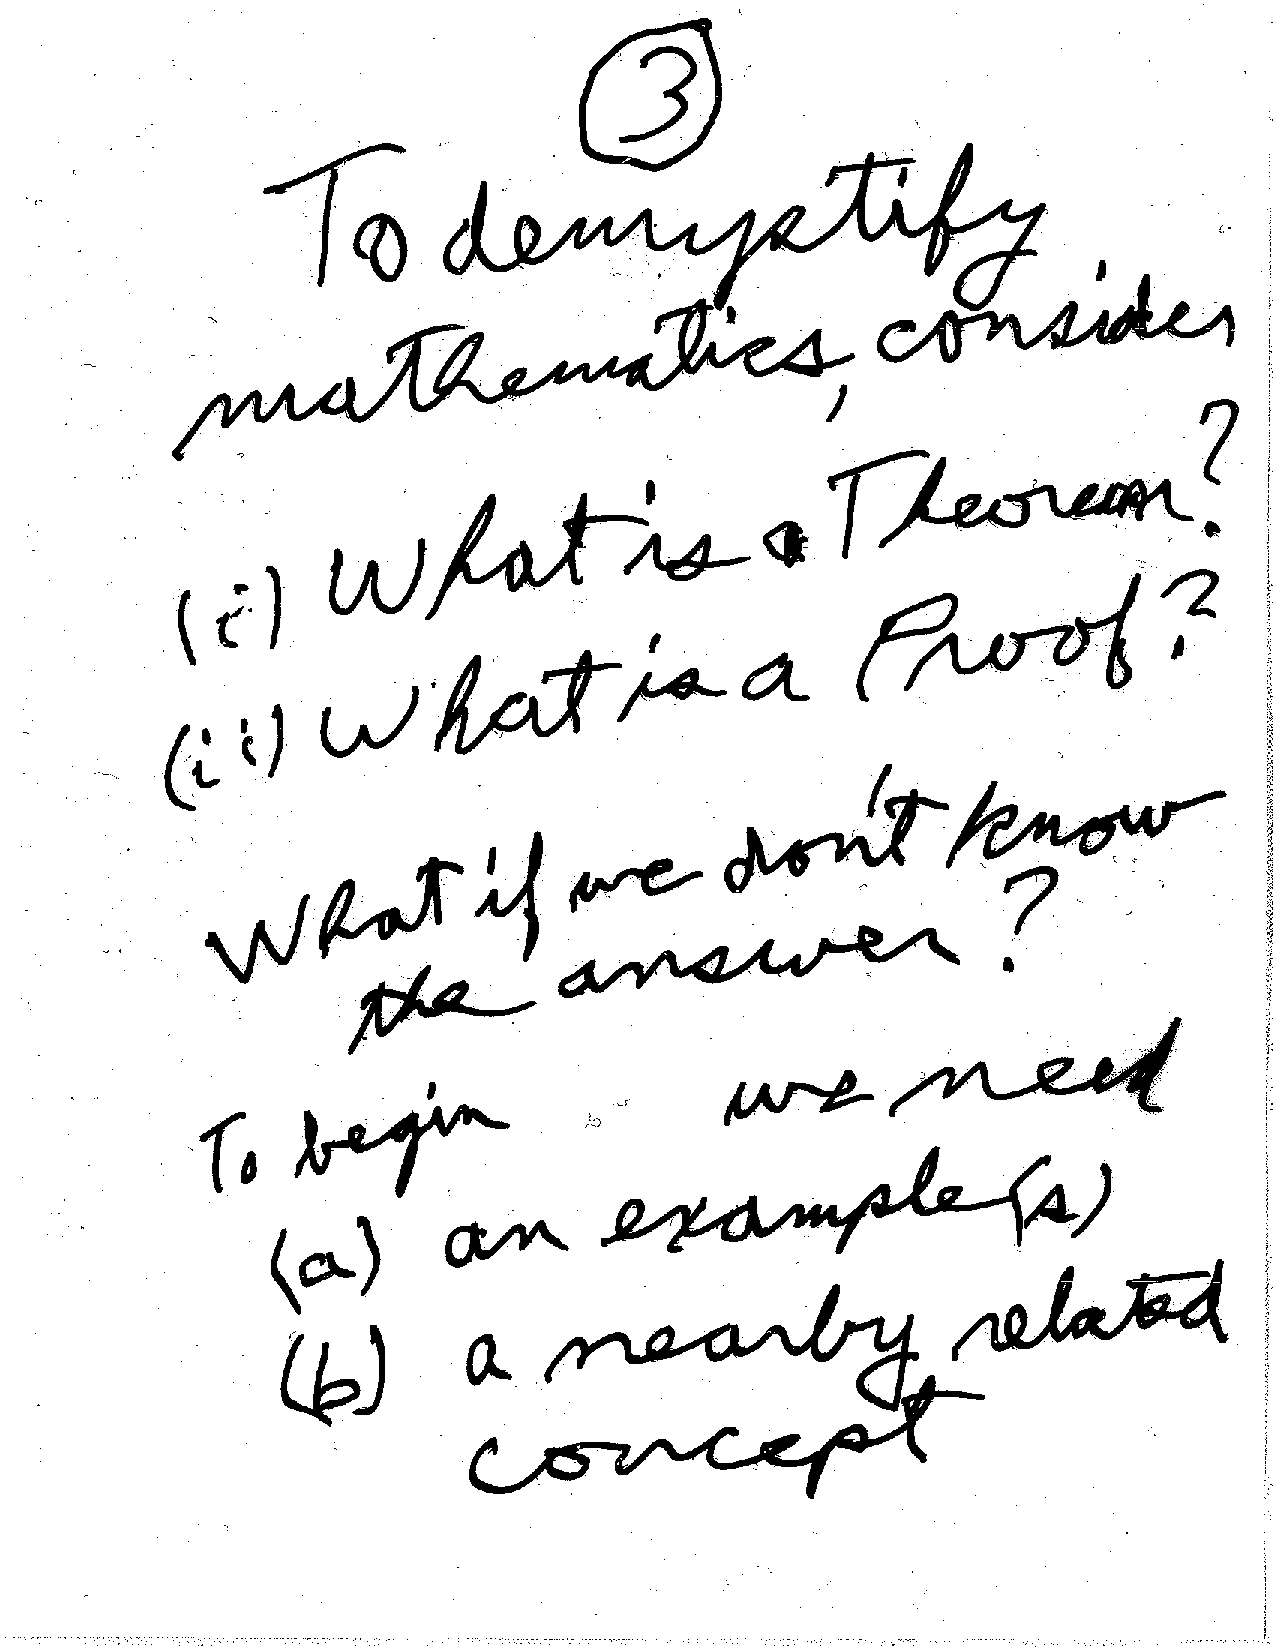
\includegraphics[scale=.5]{Pages/ST_3}

\newpage

Related Concept: Greek Syllogism

\underline{example:}
\begin{enumerate}
\item All men are mortal.
\item Socrates is a man.
\item Therefore, Socrates must die. 
\end{enumerate}

To analyze, recast in set theoretic terms via Venn Diagram.

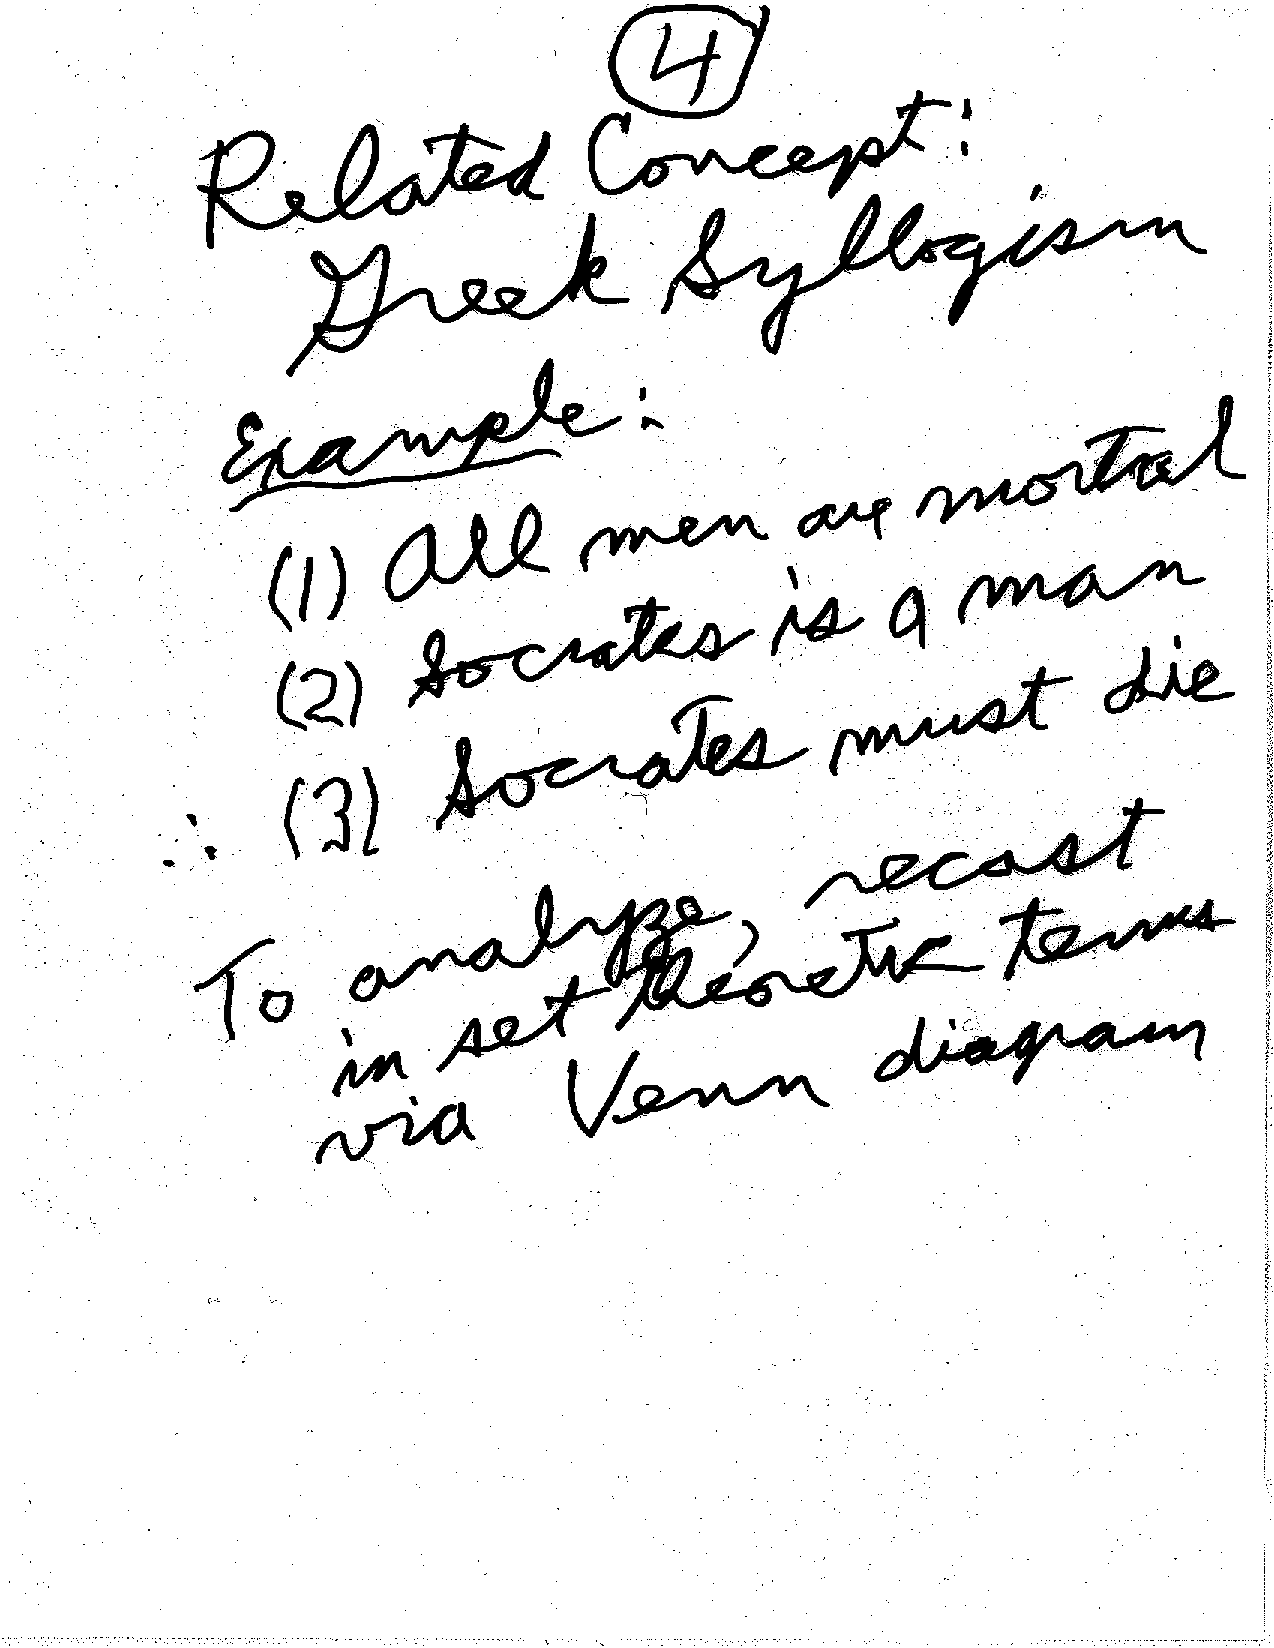
\includegraphics[scale=.5]{Pages/ST_4}

\newpage

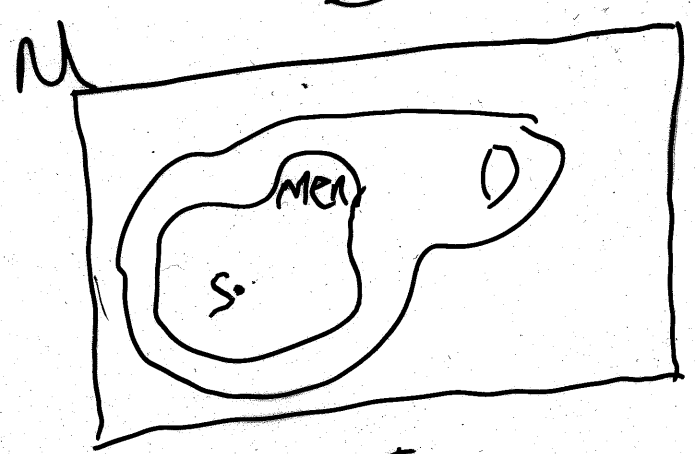
\includegraphics[scale=.2]{Pages/ST_5_im1}

$S$: Socrates\\
$M$: Set of Men\\
$D$: Things that will die\\
$\mathcal{U}$: Things on Earth

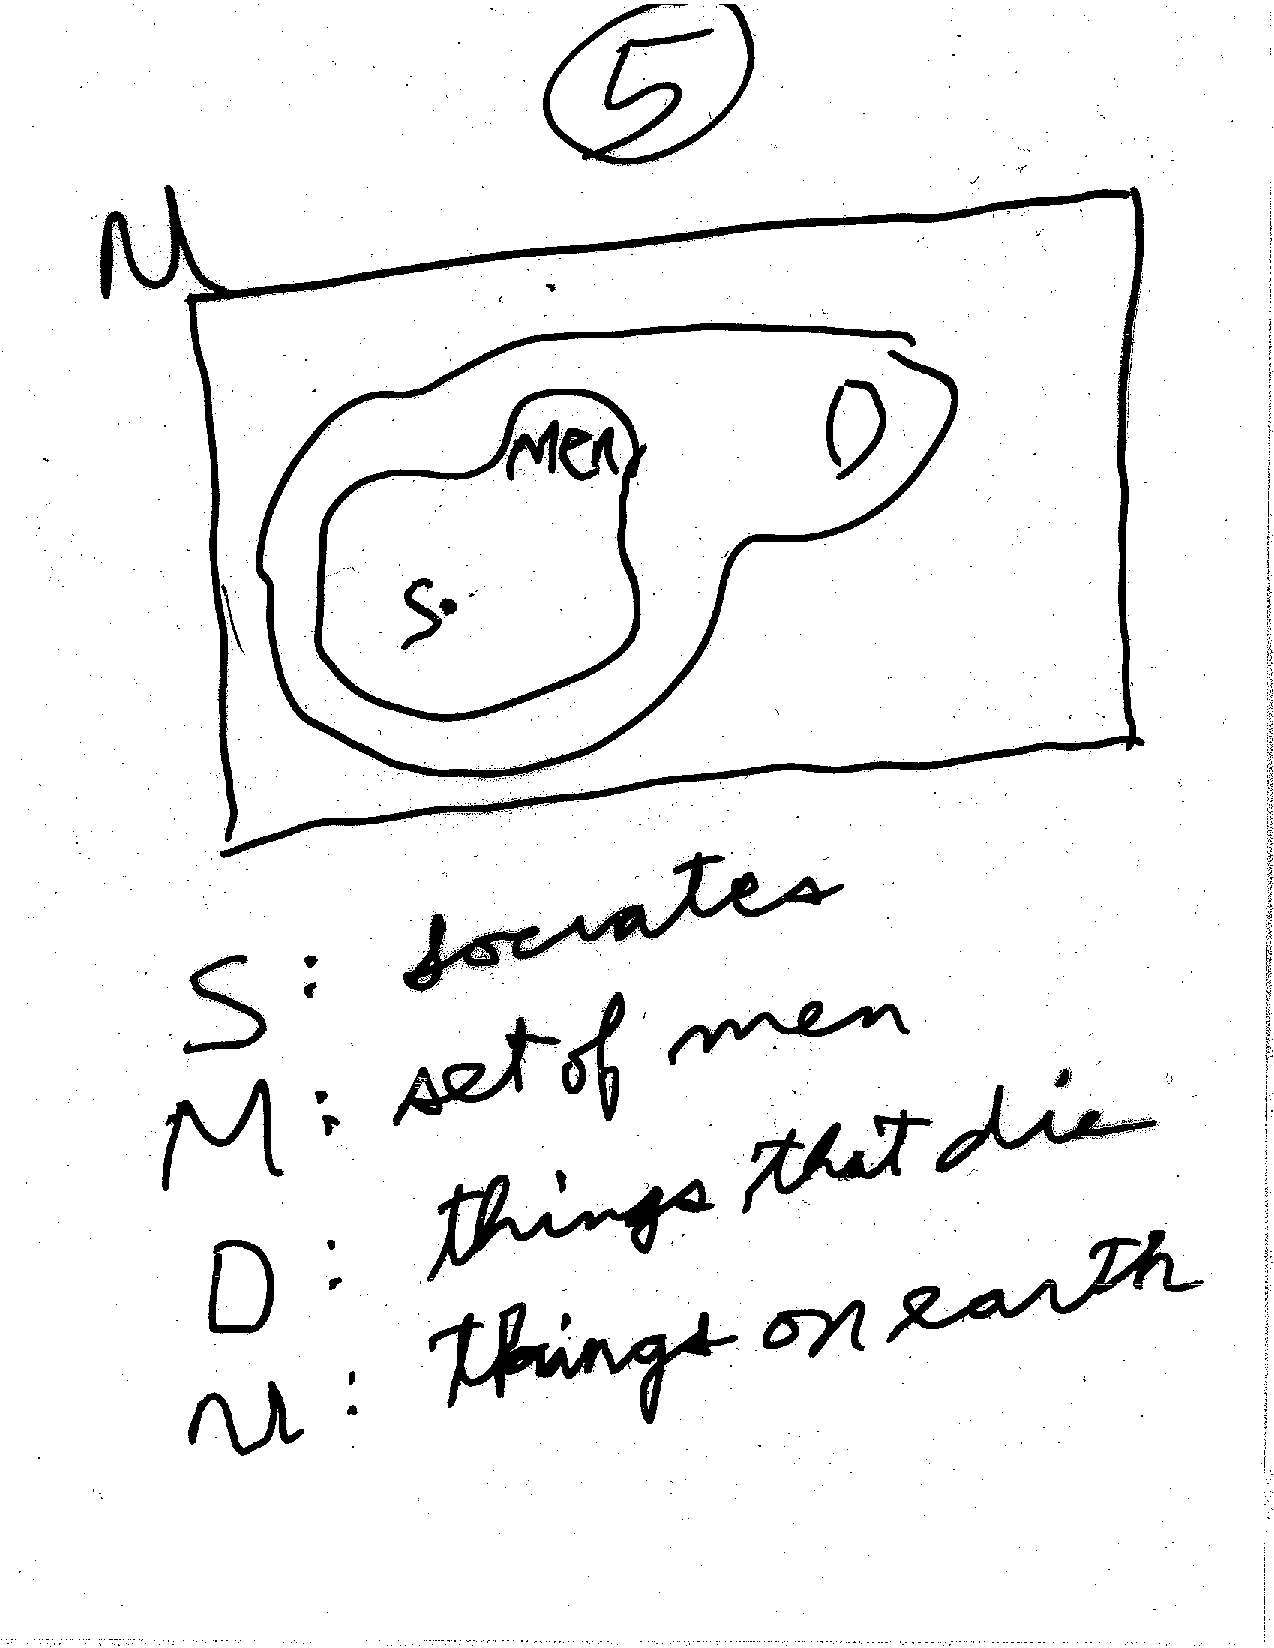
\includegraphics[scale=.5]{Pages/ST_5} 



%Zack: Pages 6,7,8,19,20
\newpage
Notice:
proper noun Socrates 
became an $\frac {element} {(point)}$

common noun \underline{men}
became a \underline{set}
(collection of pts)

\underline{the property} of being mortal became a \underline{set} the universe of all things under consider became the Universe of Possibilities 

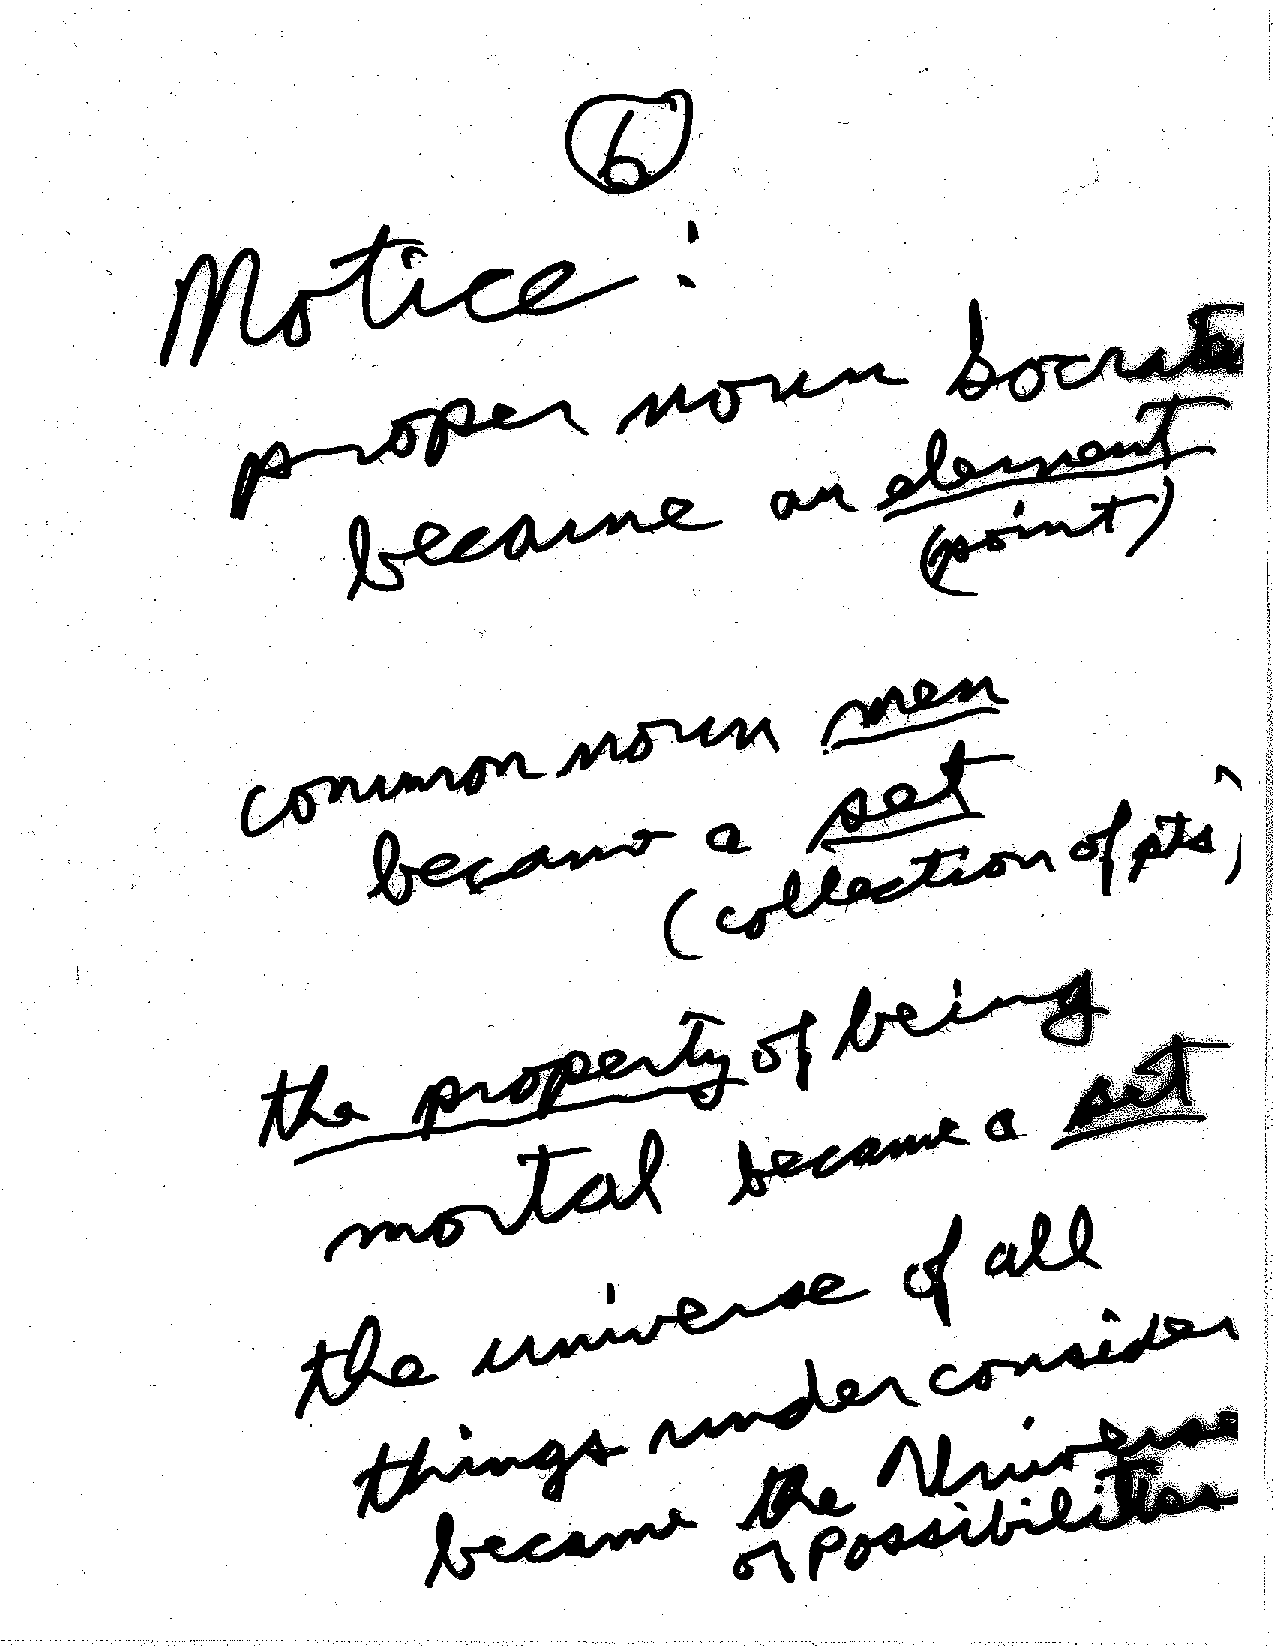
\includegraphics[scale=.5]{Pages/ST_6} 
\newpage
The set theoretic representation of the syllogism:\\
(1)$M\leq D$\\
(2)S$\varepsilon$M\\
(3)S$\varepsilon$D\\
Rearranging, we obtain a more logical ordering of the facts (doing so by successive inclusion):\\ S$\varepsilon$M, $M\leq D$; S$\varepsilon$D\\
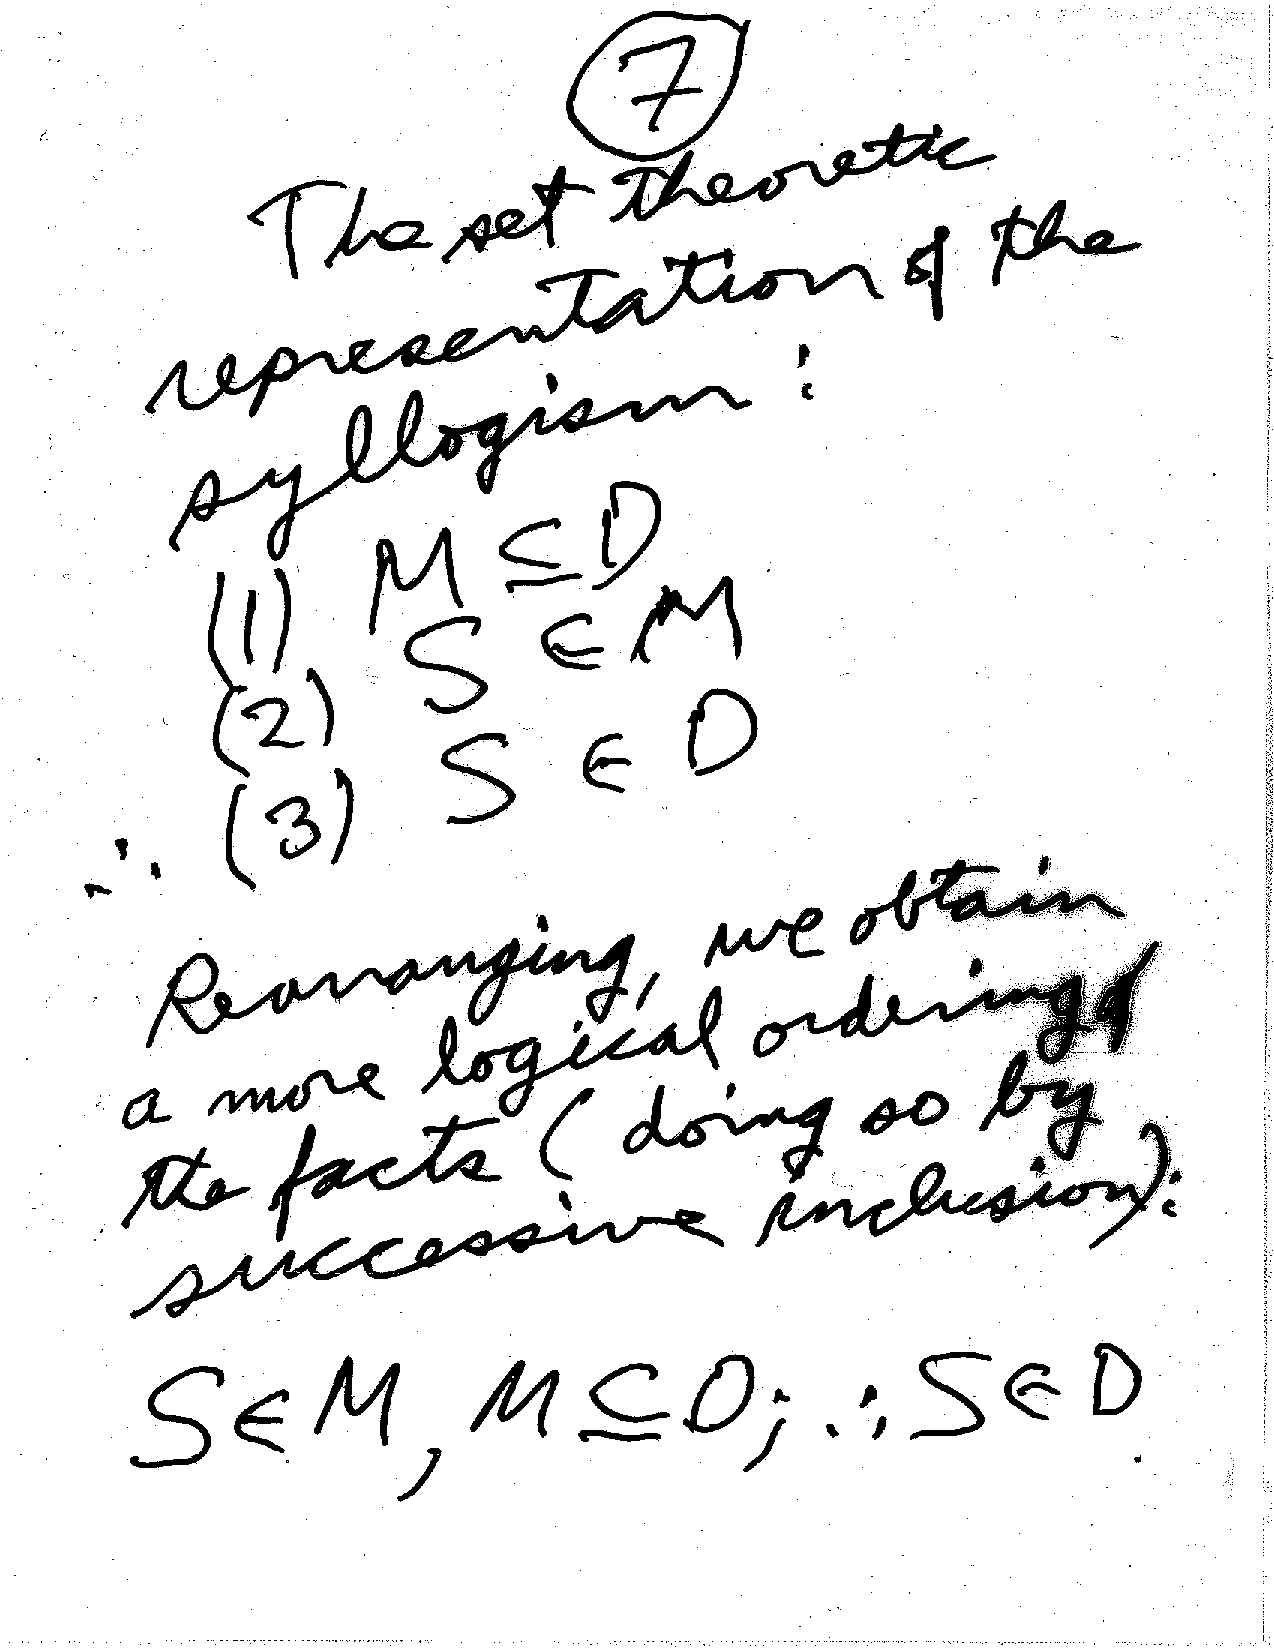
\includegraphics[scale=.5]{Pages/ST_7} 
\newpage
What has the syllogism taught us?
\begin{enumerate}
\item Games of fact (Truth on falsehood) can be put in a set theoretic context.\\
\item The simplest deductive argument has the form if $X\varepsilon$A and $A\leq B$ then $X \varepsilon$ B
\end{enumerate}
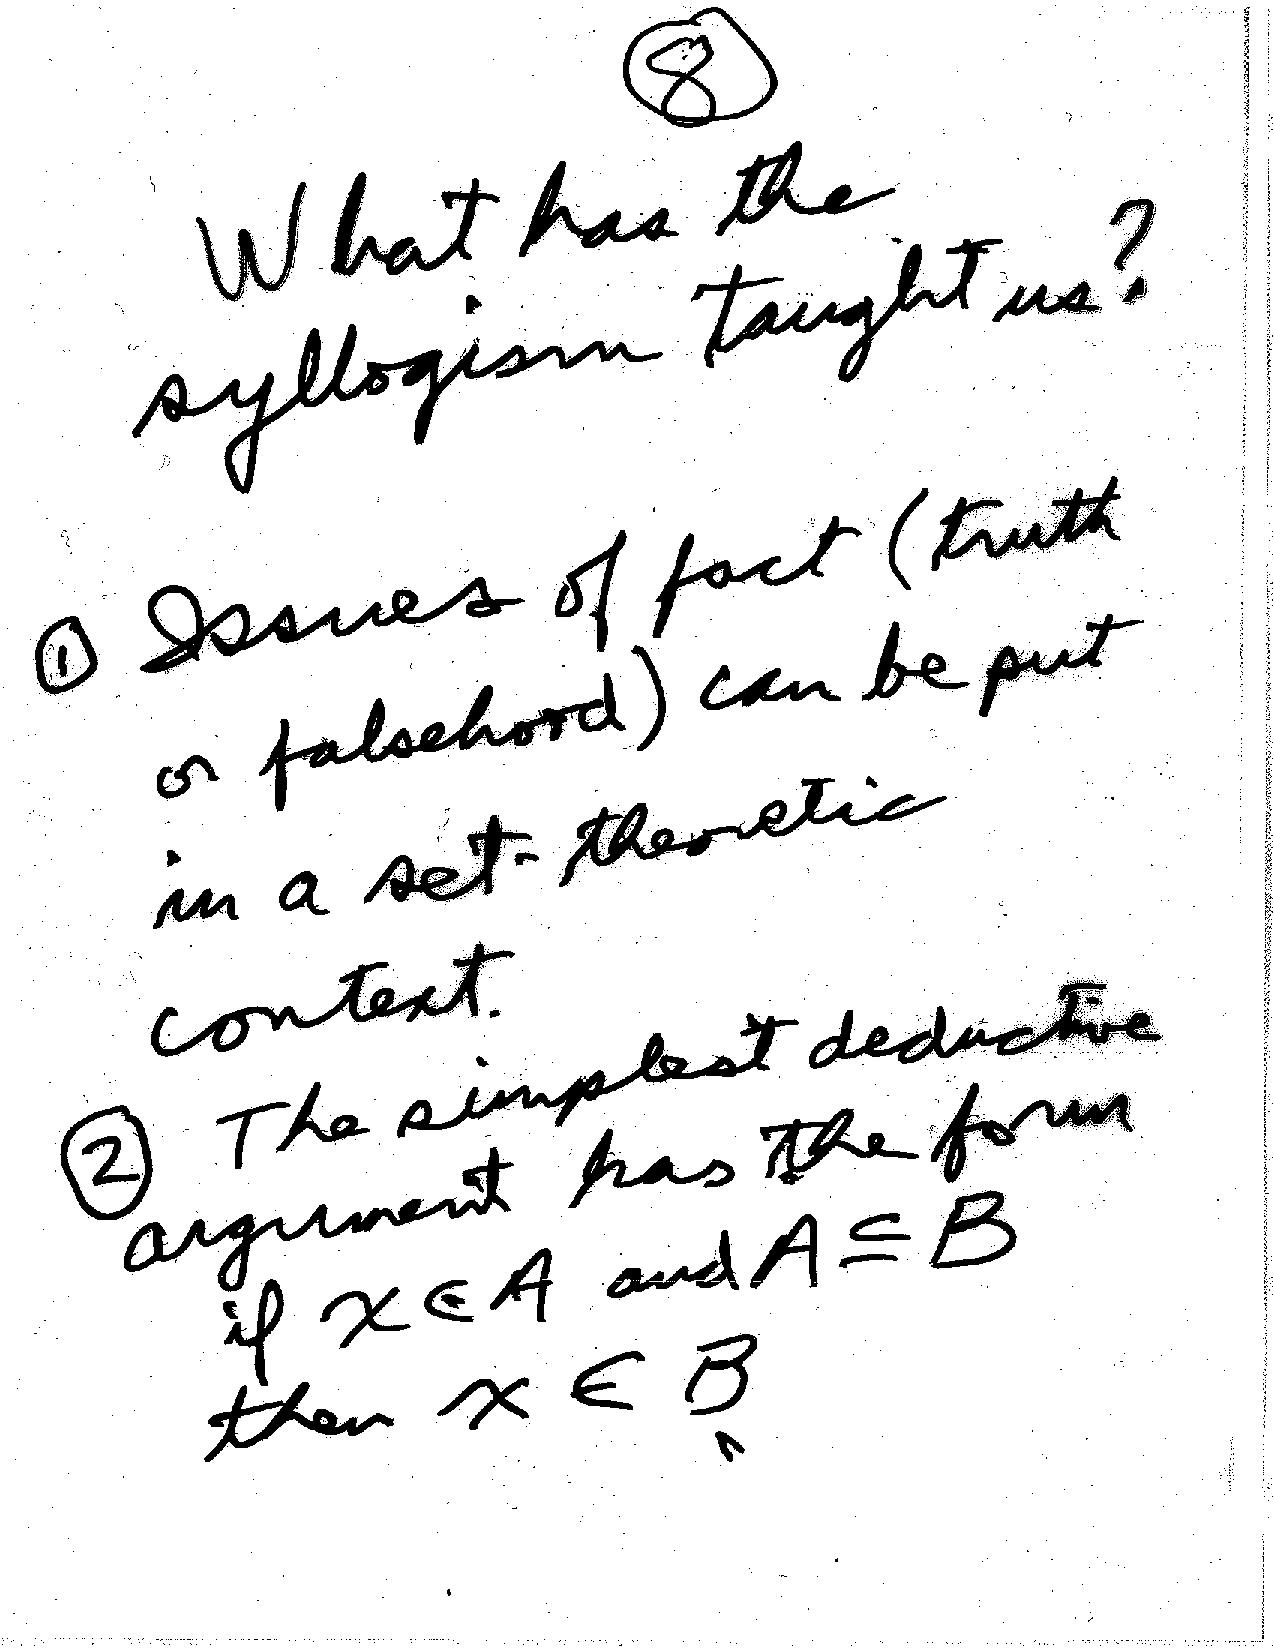
\includegraphics[scale=.5]{Pages/ST_8}


%Jack: 21, 9, 10, 11

%Koka: Pages 13, 13A, 22 ,22A, 22B

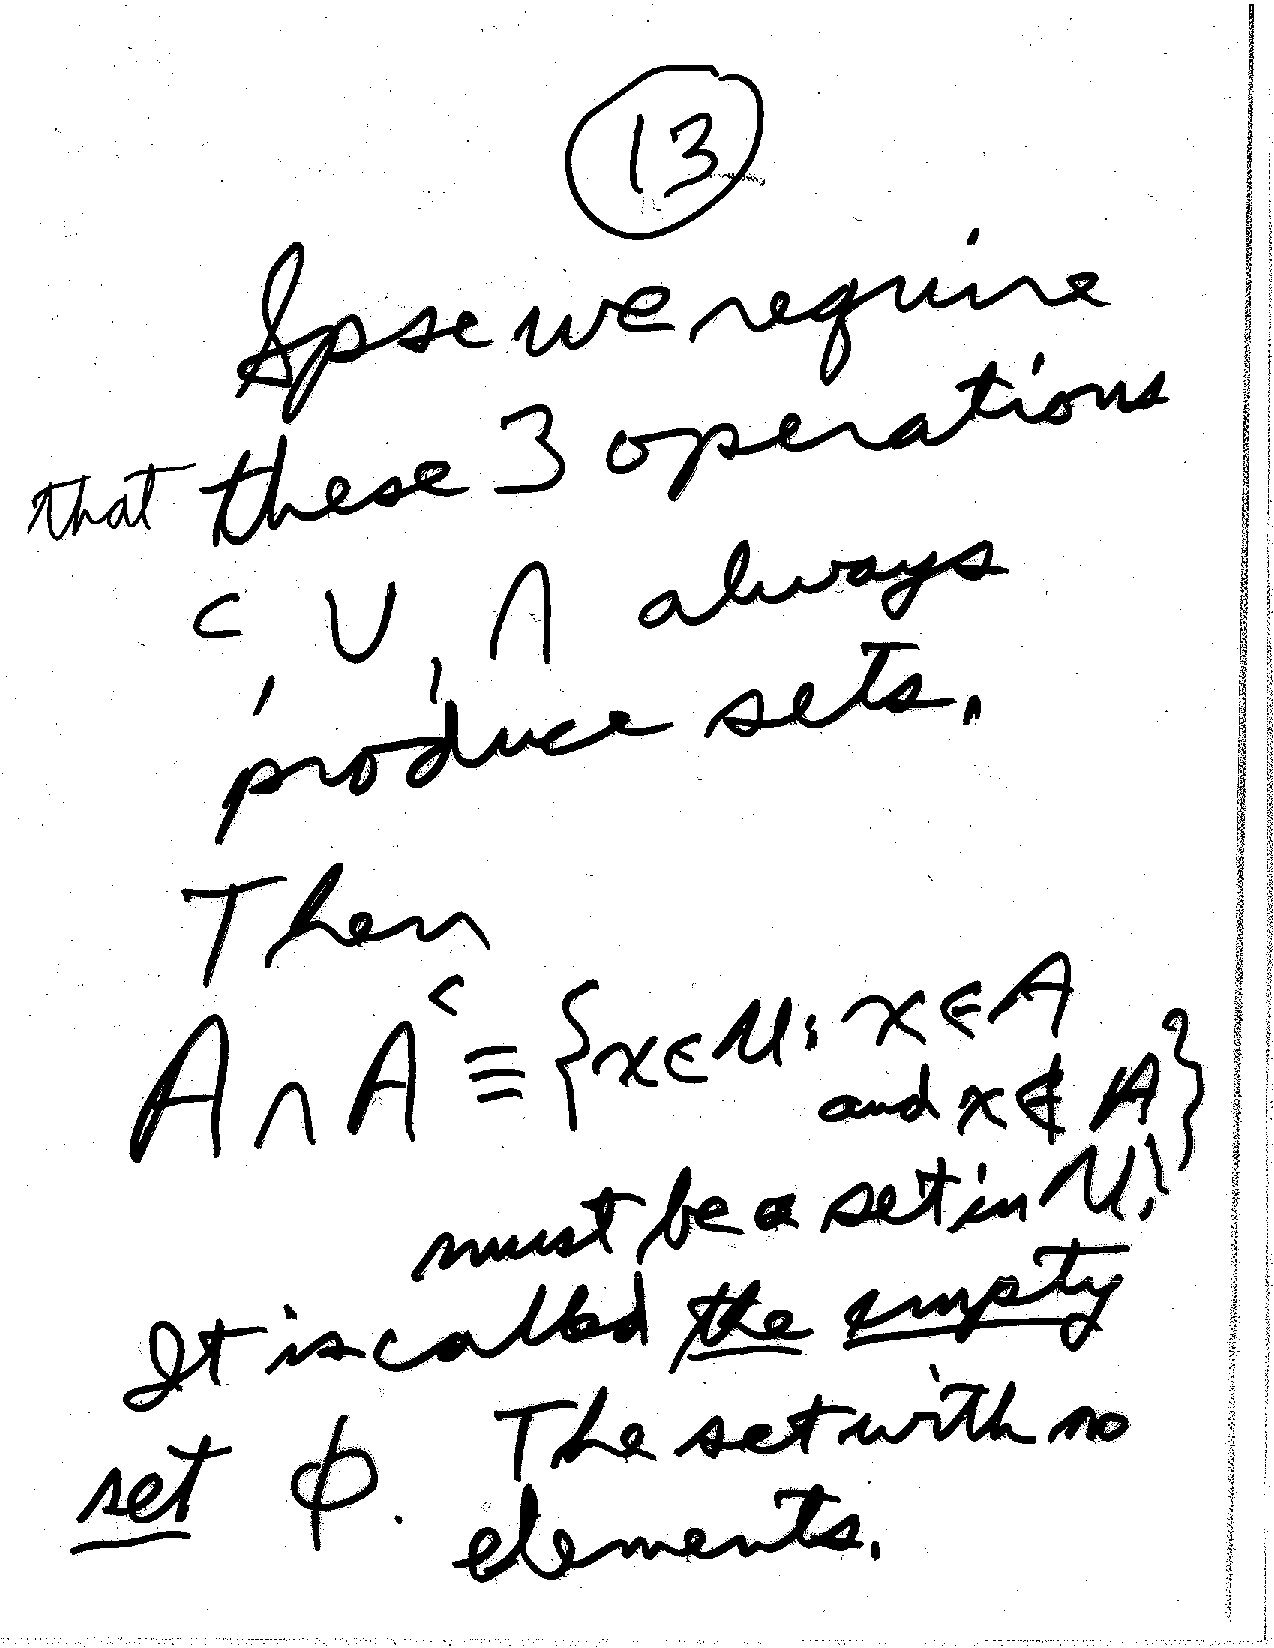
\includegraphics[scale=.5]{Pages/Page_13}

13. Suppose we require that these 3 operations $^C , \bigcup , \bigcap$ always produce sets. Then $A \bigcap A^C \equiv \{ x \in u:x \in A$ and $x \notin $ must be a set in U. 
It is called \underline{the empty set} $\emptyset$. The set with no elements. 

\vspace{.20 in}

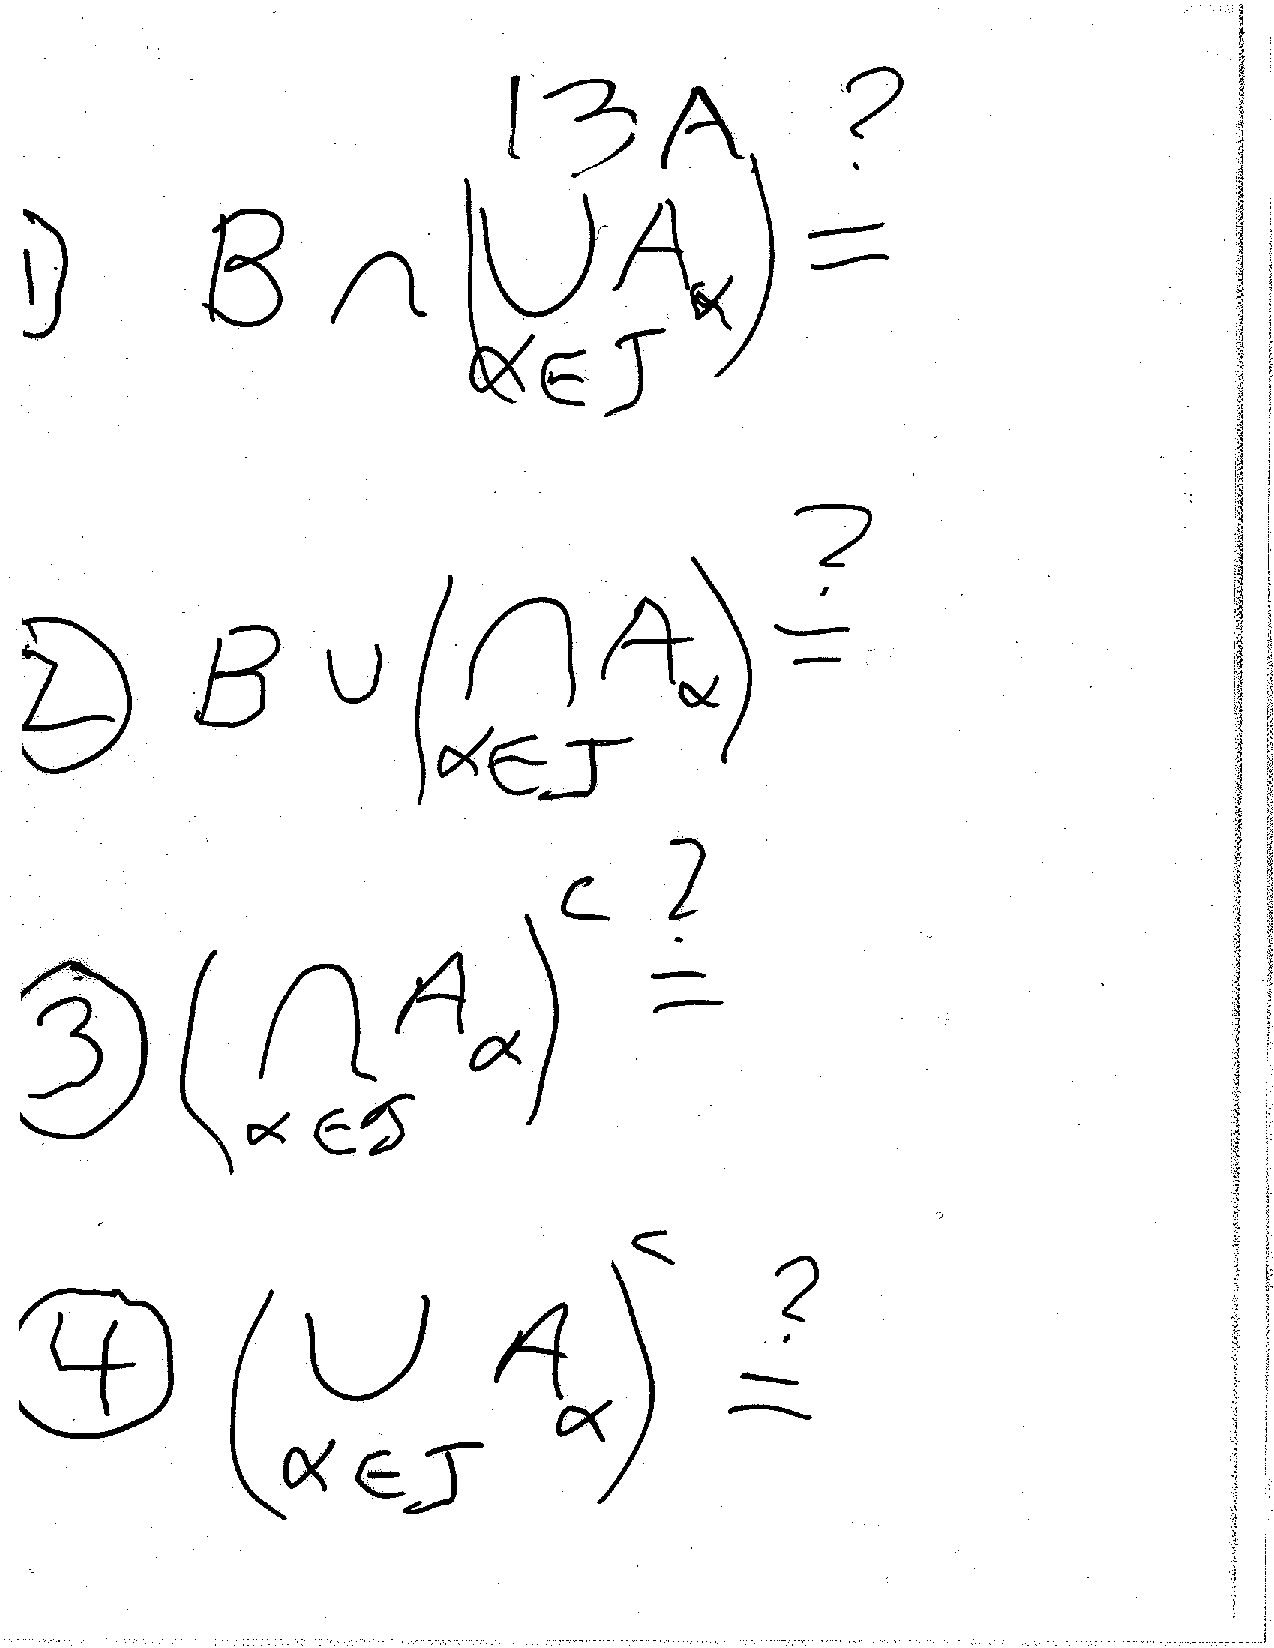
\includegraphics[scale=.5]{Pages/Page_13A}

13A. 
\begin{enumerate}
\item $$B \bigcap (\bigcup_{\alpha \in J} A_\alpha) \stackrel{?}{=}$$
\item $$B \bigcup (\bigcap_{\alpha \in J} A_\alpha) \stackrel{?}{=}$$
\item $$(\bigcap_{\alpha \in J} A_\alpha)^c \stackrel{?}{=}$$
\item $$(\bigcup_{\alpha \in J} A_\alpha)^c \stackrel{?}{=}$$
\end{enumerate}

\vspace{.20 in}

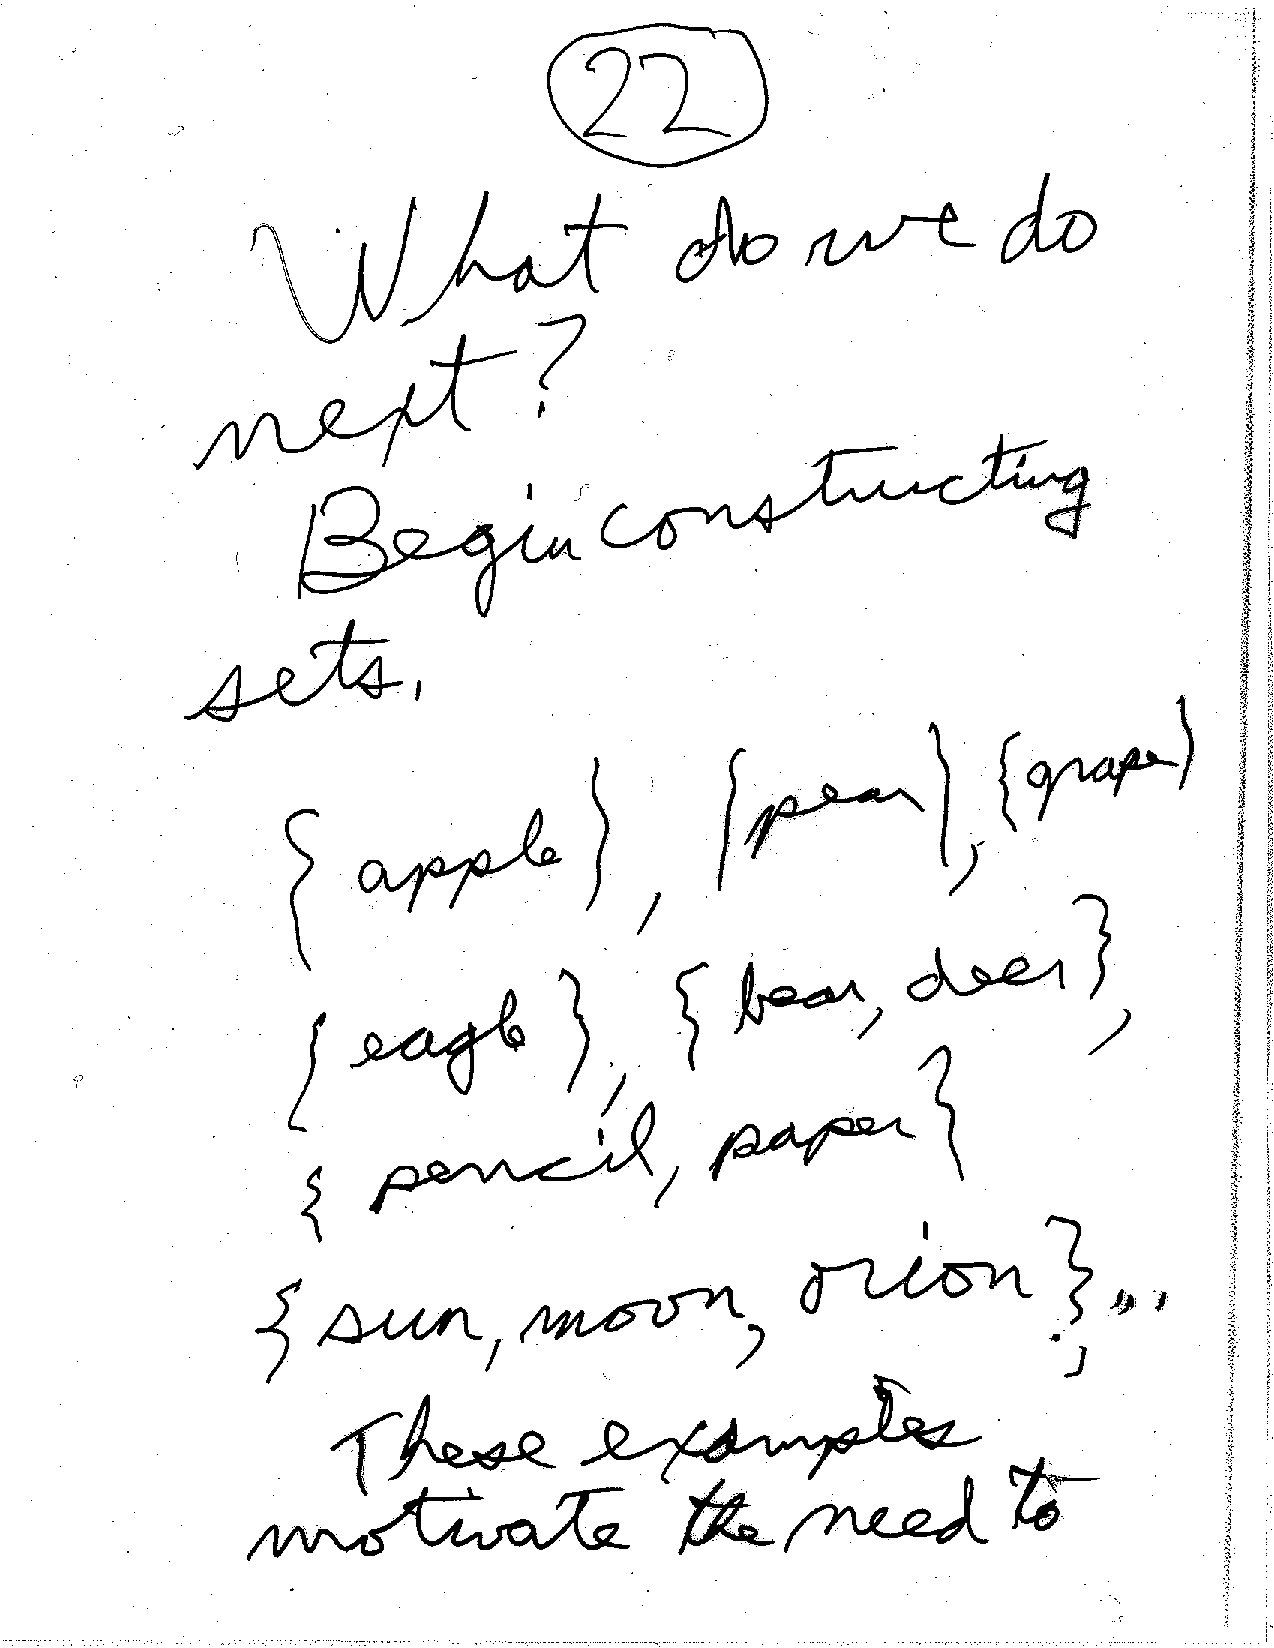
\includegraphics[scale=.5]{Pages/Page_22}

22. What do we do next? Begin constructing sets, $\{$ apple $\}$ , $\{$ pen $\}$, $\{$ grape $\}$, $\{$ eagle $\}$, $\{$ bear, deer $\}$, $\{$ pencil, paper $\}$, $\{$ sun, moon, onion. $\}$ These examples motivate the need to

\vspace{.20 in}

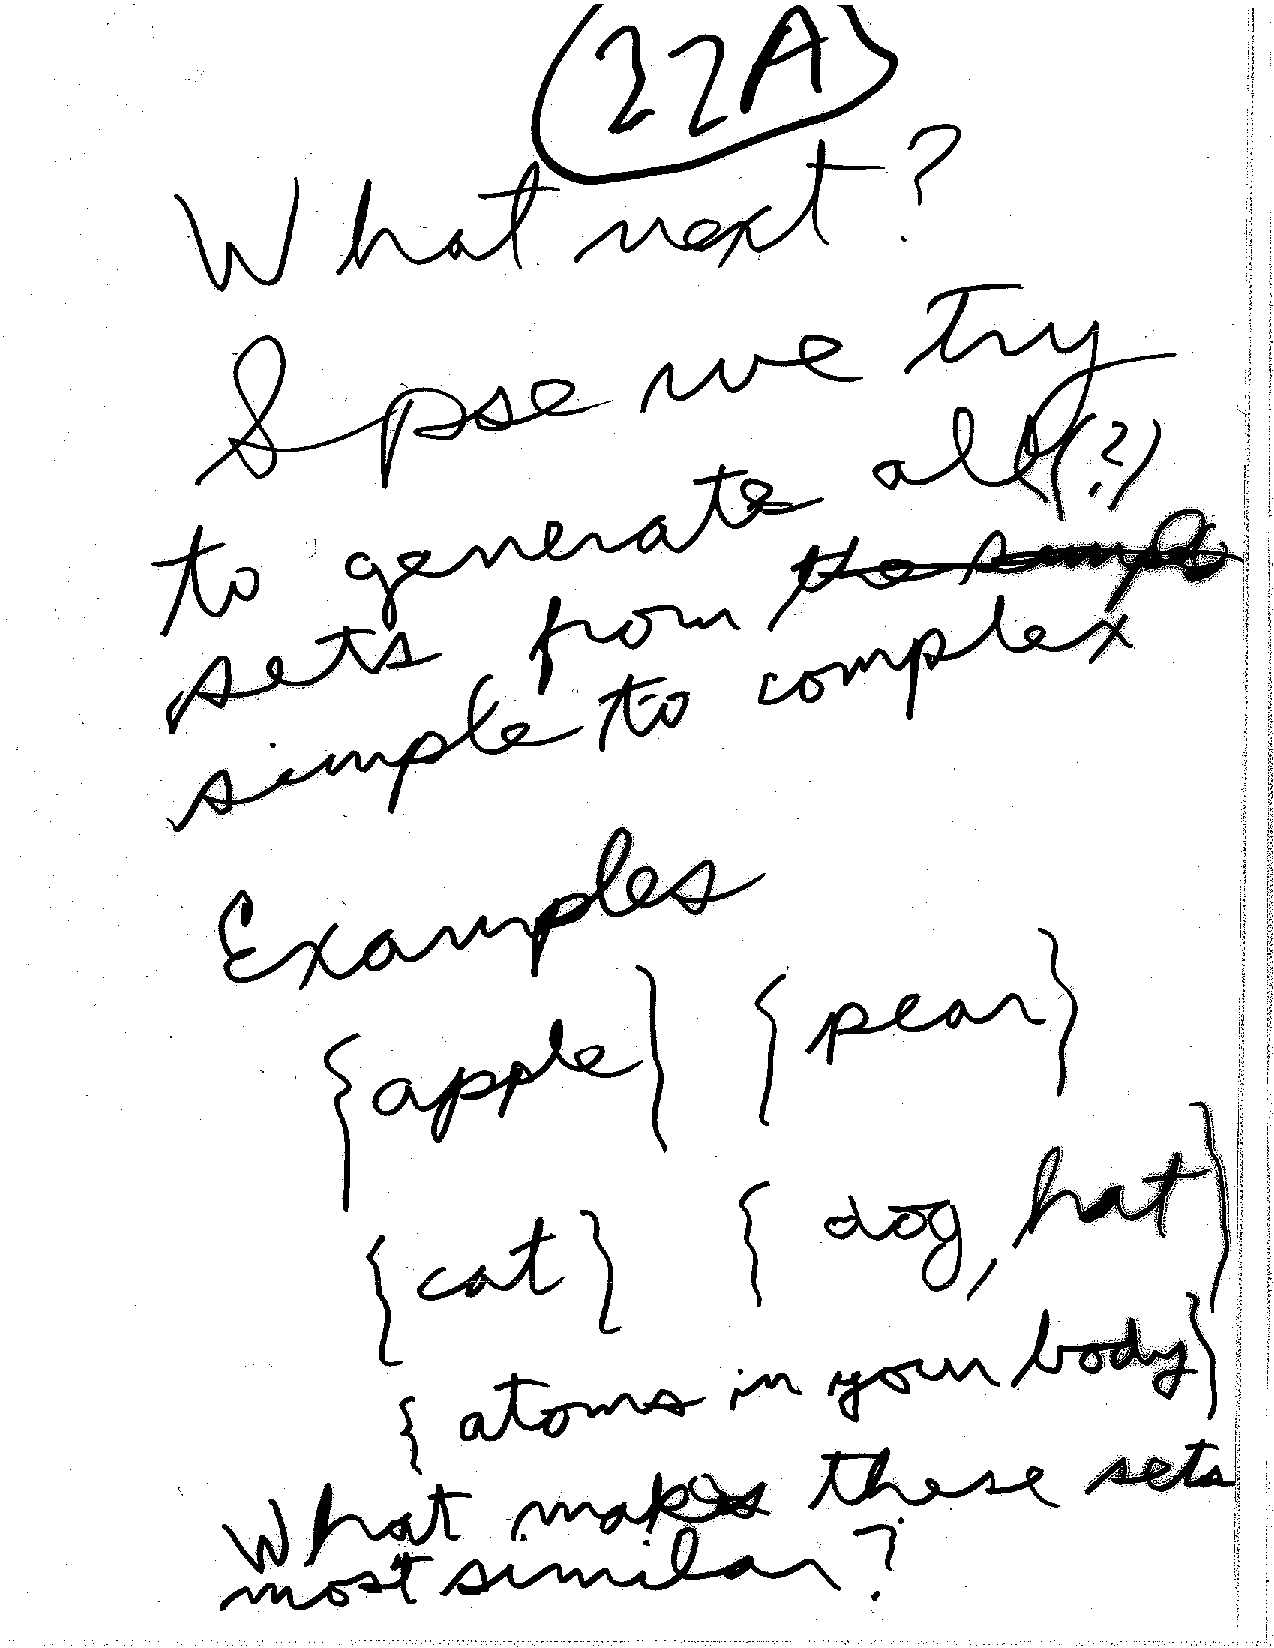
\includegraphics[scale=.5]{Pages/Page_22A}

22A. What next? Suppose we try to generate all sets from simple to complex Examples $\{$ apple $\}$  $\{$ pear $\}$ $\{$ cat $\}$ $\{$ dog,hat $\}$ $\{$ atoms in your body $\}$ What makes these sets most similar? 

\vspace{.20 in}

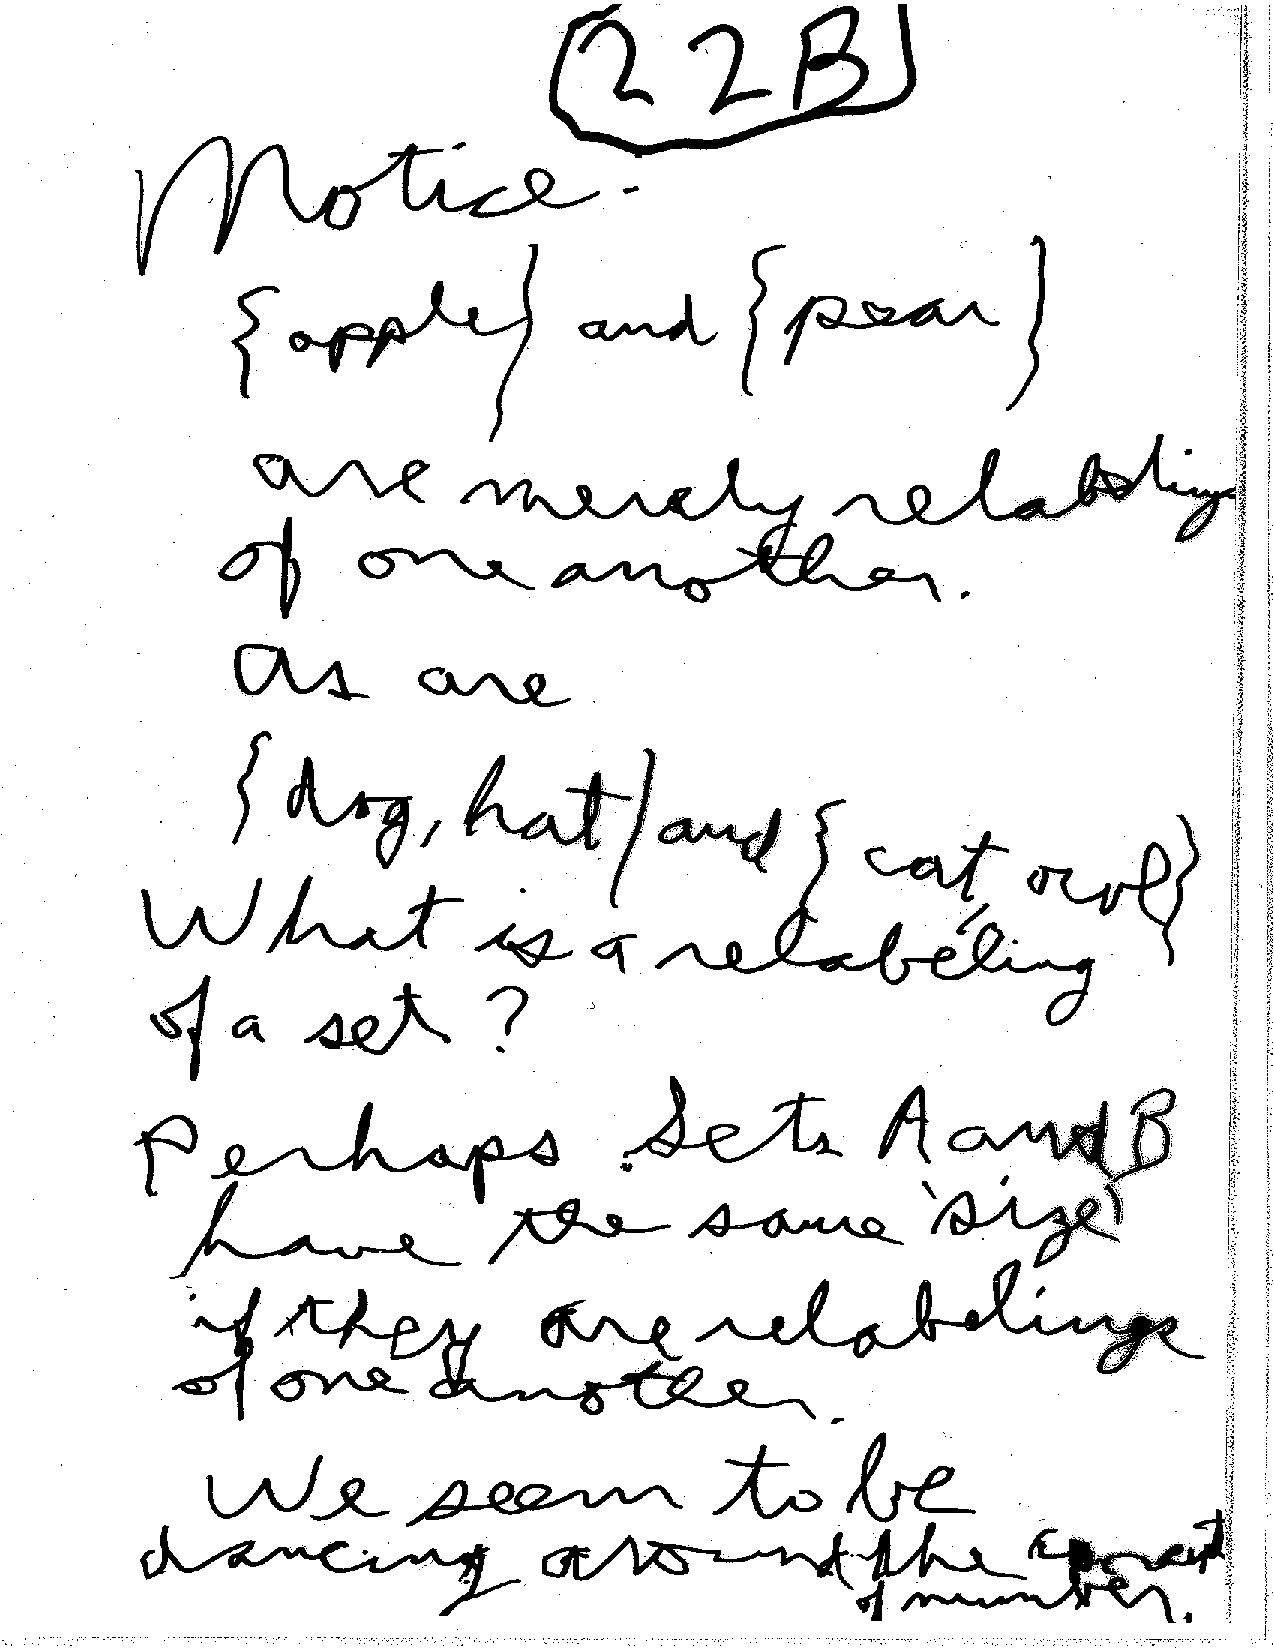
\includegraphics[scale=.5]{Pages/Page_22B}

22B. Notice $\{$ apple $\}$ and $\{$ pear $\}$ are merely relating of one another as one $\{$ dog, hat $\}$ and $\{$ cat, oval $\}$ What is a relabeling of a set? Perhaps sets A and B have the same 'size' if they are relabeling of one another. We seem to be dancing around the concept of number. 

\section{Generate $\mathbb{N}$}


%Ruth: Pages L4A-L4G
\begin{Large}
L4A Generate $\mathbb{N}$
\end{Large}

\textit{$\mathbb{N}$}= $\lbrace$ 1, 2, 3,.. $\rbrace$ as produced via Peono Axions. How do the set theorists generate $\mathbb{N}$ Hint: Use 
$\phi$ Is there any inherent/essential/intrinsic difference between $\lbrace$cat, hat, dog, blue$\rbrace$ and $\lbrace$1, 2, 3, 4$\rbrace$?

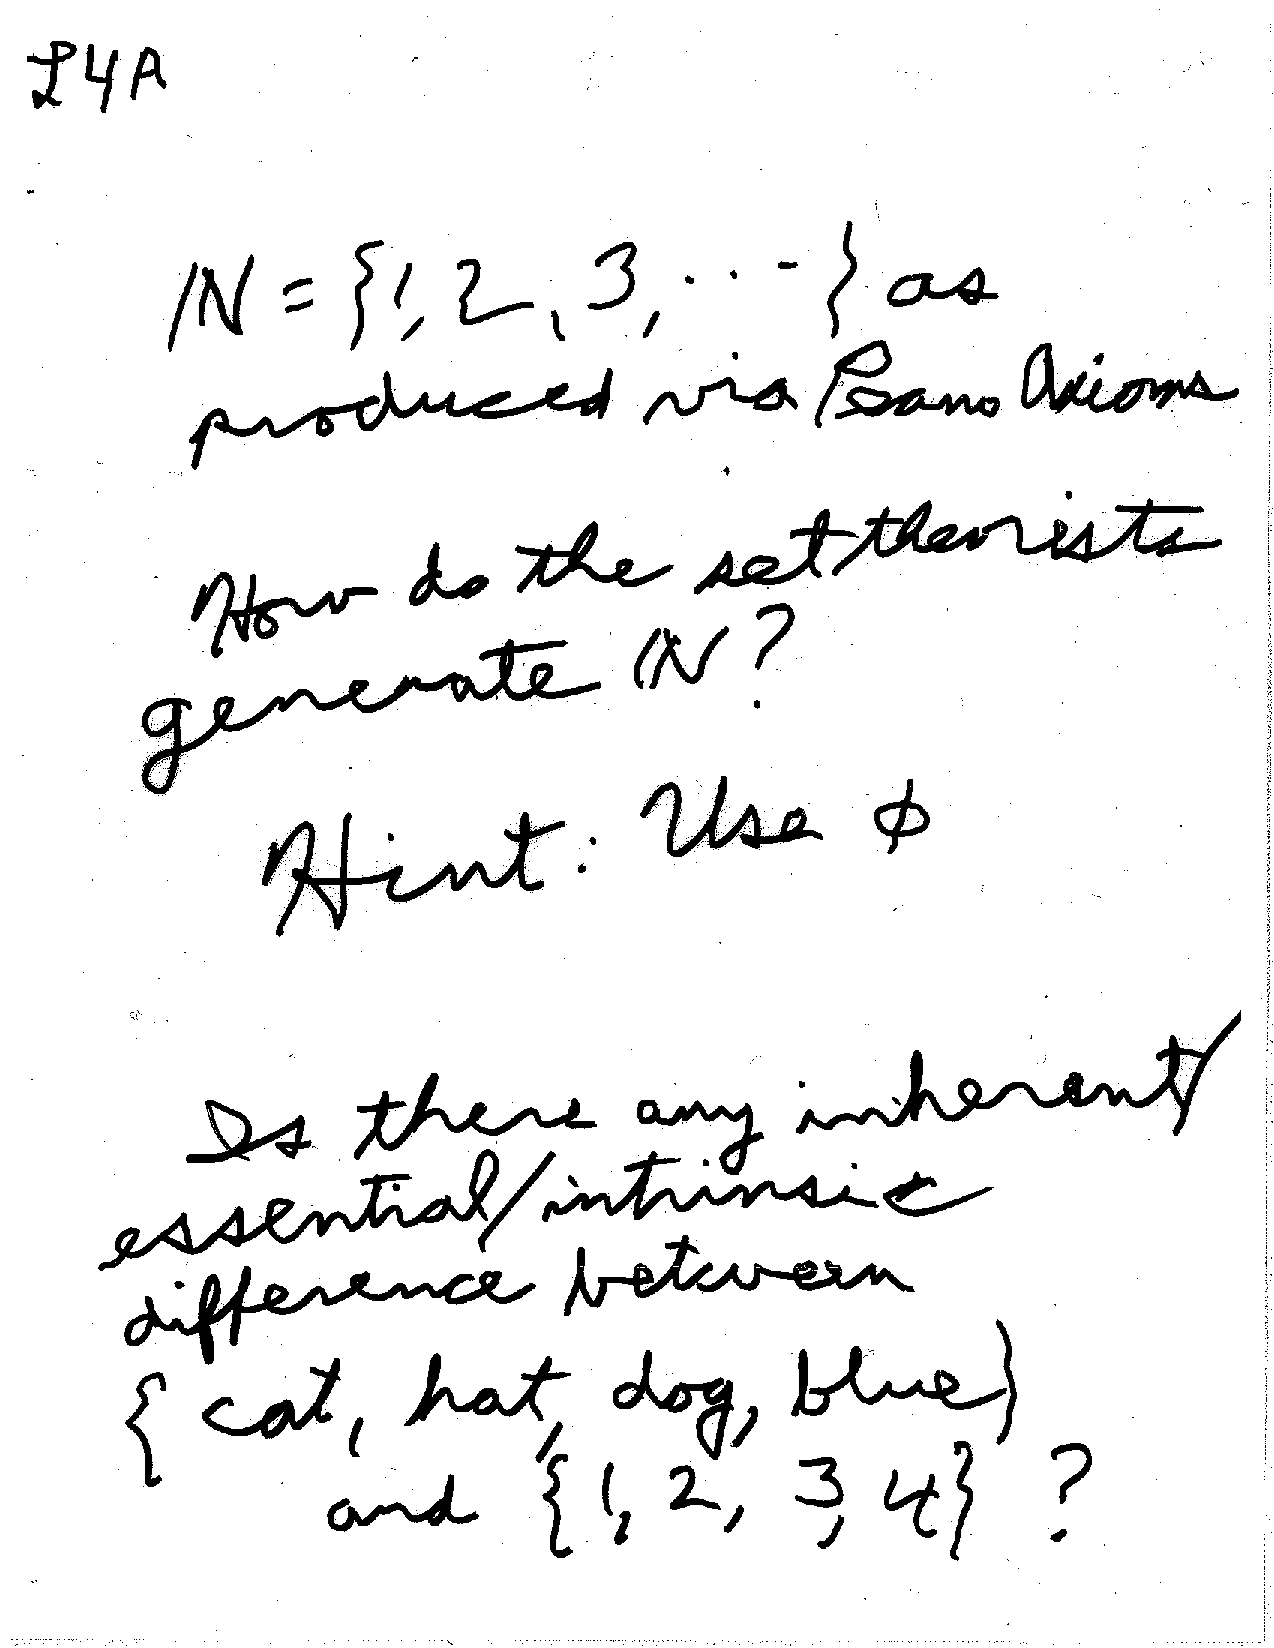
\includegraphics[scale=0.5]{Pages/generateN1.pdf}

\newpage

\begin{Large}
L4B Generate $\mathbb{N}$
\end{Large}

Ans.One set has an implicit ordering induced by Peono Axions.
Def: $<$is a (strict) ordering on $S$ (S $\neq$ $\emptyset$) if $\forall$ a, b, c in S 

\begin{enumerate}[(i)]
\item Exactly one of 

a $<$ b

b $<$ a

a = b is true 
\item If a $<$ b and b $<$ c 
\end{enumerate}
then a $<$ c
This is an axiomatic presentation

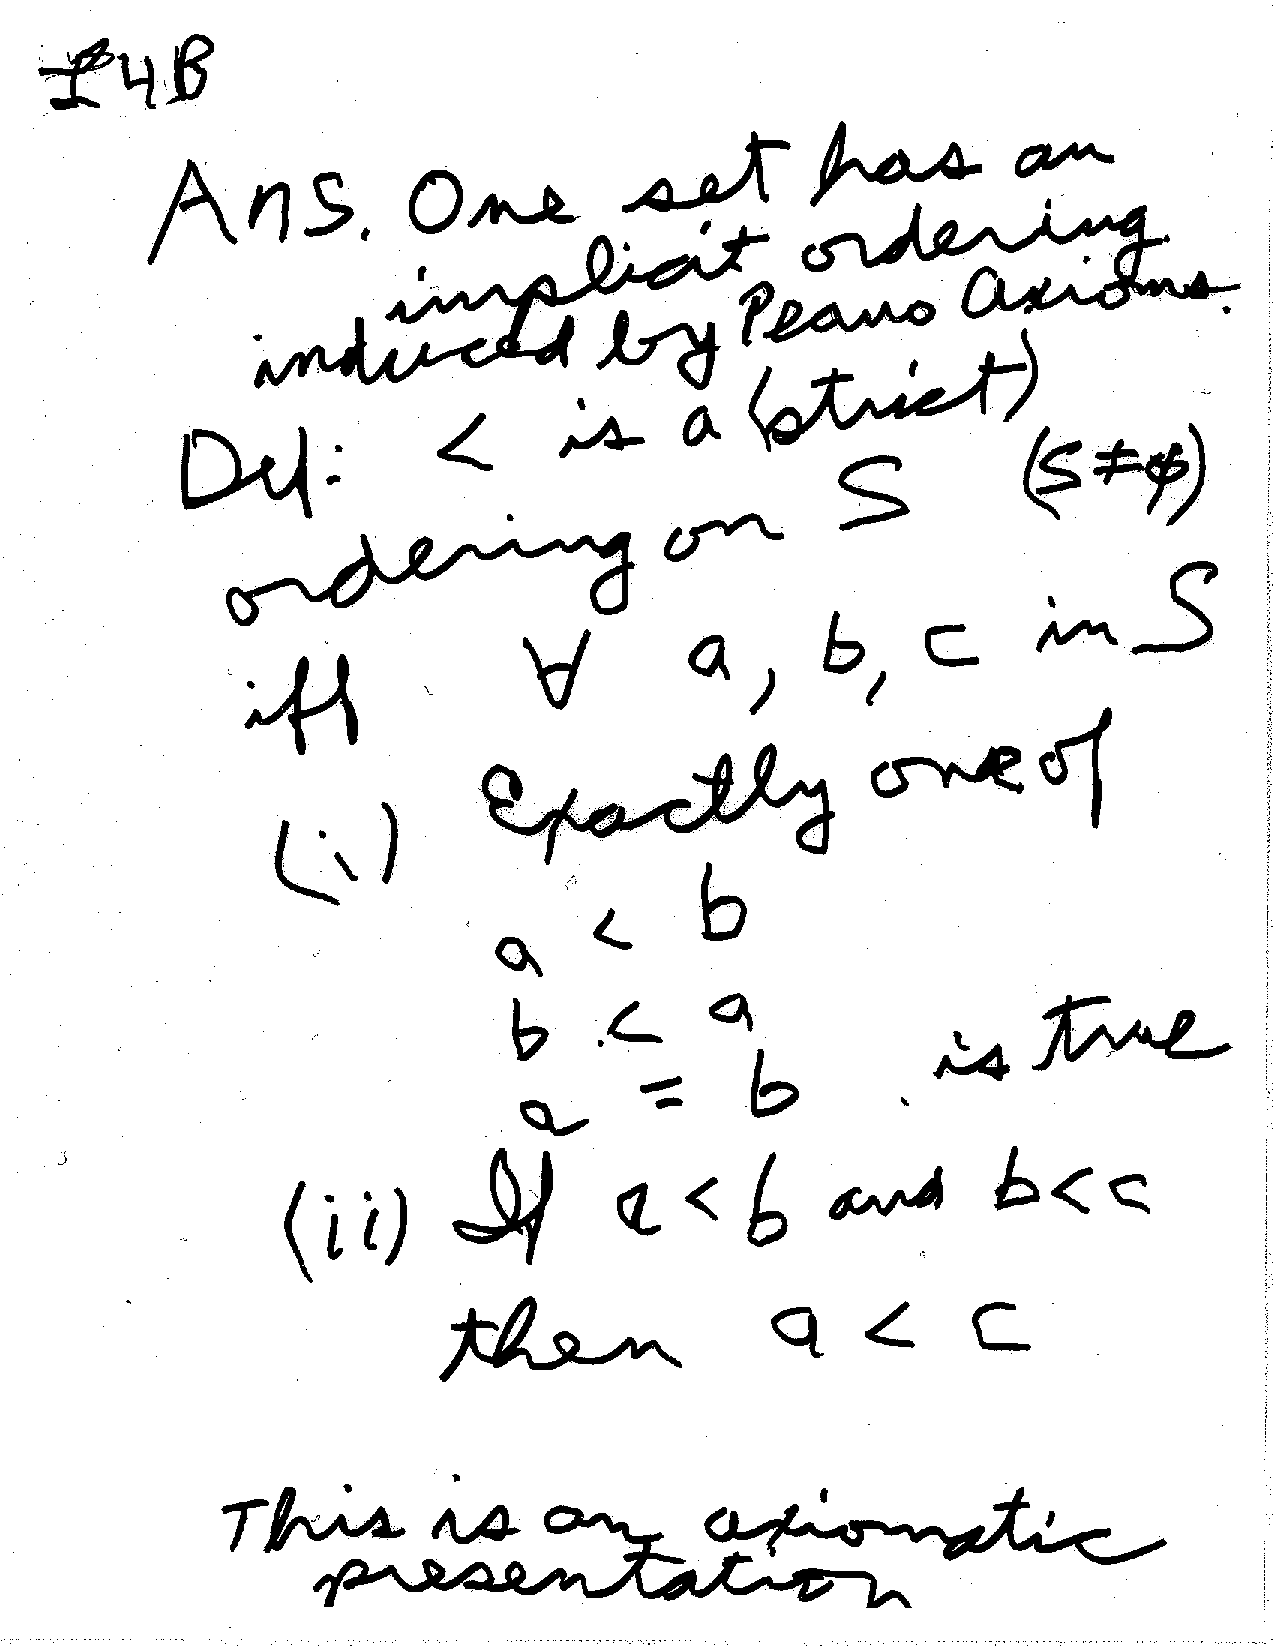
\includegraphics[scale=0.5]{Pages/generateN2.pdf}

\newpage

\begin{Large}
L4C Generate $\mathbb{N}$
\end{Large}

How could this notion be achieved set theoretically? Note: It involves pairs of elements of S.

1st step 
Need $<$ to be a subset 6 of $SxS$ = (S{\begin{tiny}
1 
\end{tiny}
S{\begin{tiny}
2
\end{tiny})
For all a, b, c in S
\begin{enumerate}
\item[(i)] 
(a, b) $\epsilon$ 6 
if (b, a) 6 $\nexists$ 
\item[(ii)] 
if (a, b) and (b, c) $\epsilon$ C then (a, c) $\epsilon$ C
\end{enumerate}

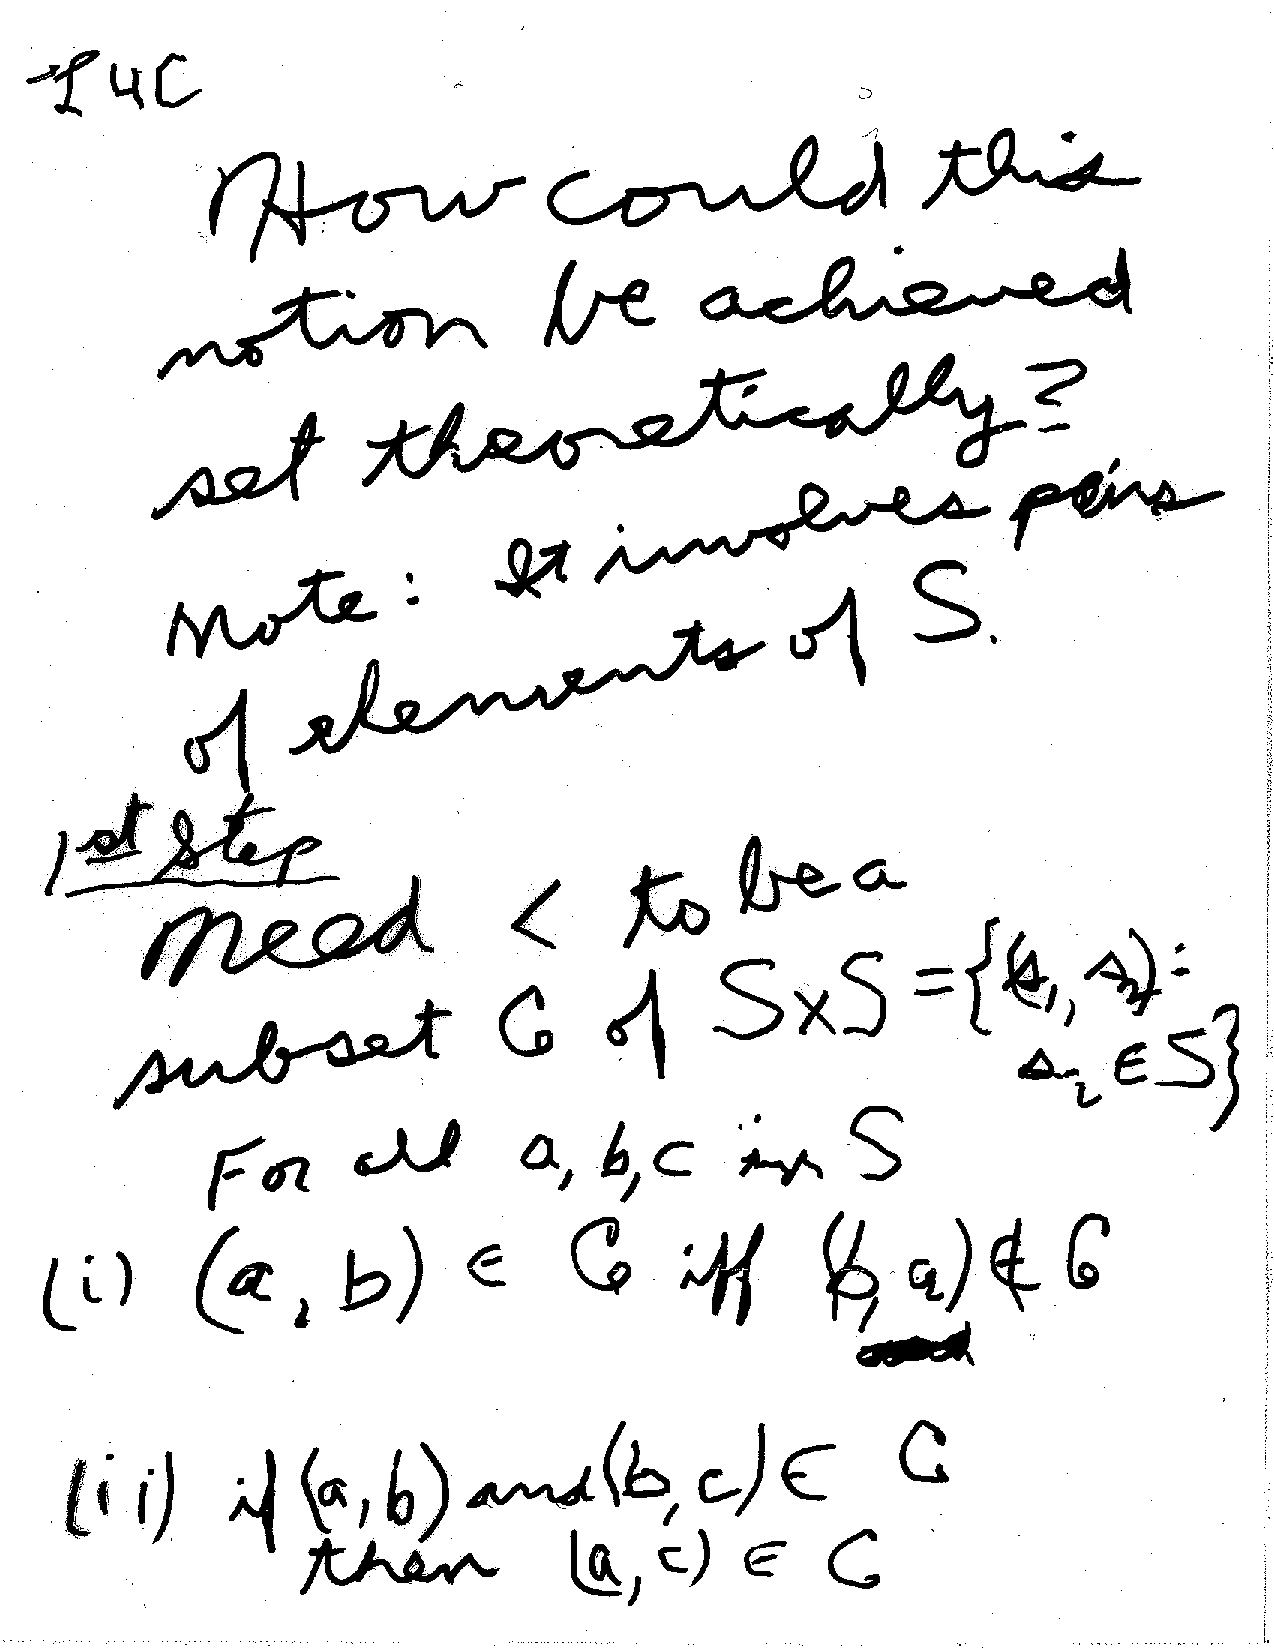
\includegraphics[scale=0.5]{Pages/generateN3.pdf}

\newpage

\begin{Large}
L4D Generate $\mathbb{N}$
\end{Large}

Step 2 Sets are Undefined Present $A \times B$ (and so $S \times S$) set theoretically: (a, B) can be re-exposed so that its order on this surface does not affect its meaning How? for example consider $\lbrace$ $\lbrace$ a, 1 $\rbrace$, $\lbrace$ b, 2 $\rbrace$
$\rbrace$ instead of (a, b) or even $\lbrace$ a\begin{tiny}
2
\end{tiny}
$\lbrace$a, b$\rbrace$
$\rbrace$ to denote a typical element of AxB

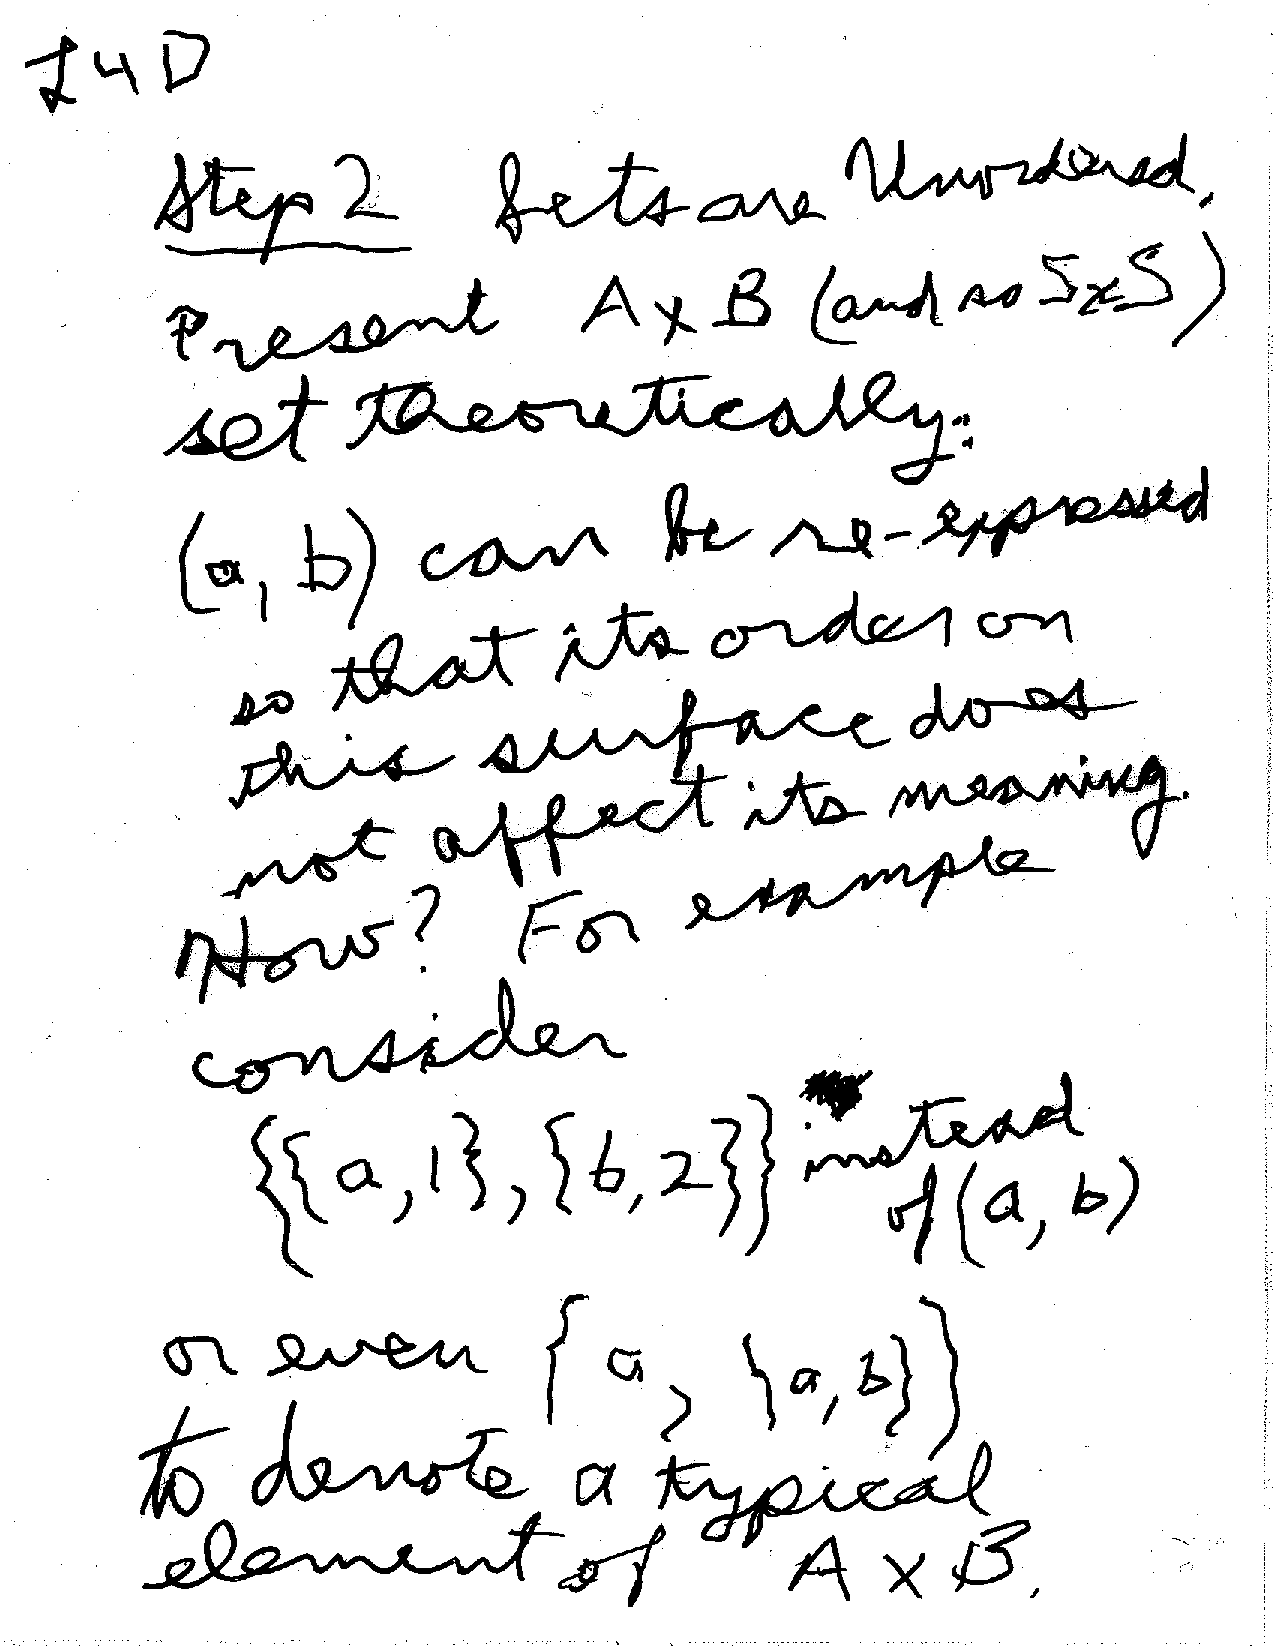
\includegraphics[scale=0.5]{Pages/generateN4.pdf}

\newpage

\begin{Large}
L4E Generate $\mathbb{N}$
\end{Large}
Most importantly the set S can be reconstructed to exhibit its order For example give (S, $<$) and s $\in$ S let Ls
= $\lbrace$ a $\in$ S; a $<$ s $\rbrace$ Then let $S$ = $\lbrace$ Ls
: s $\in$ S $\rbrace$ (S, c) represents (S, $<$) Can you find another?
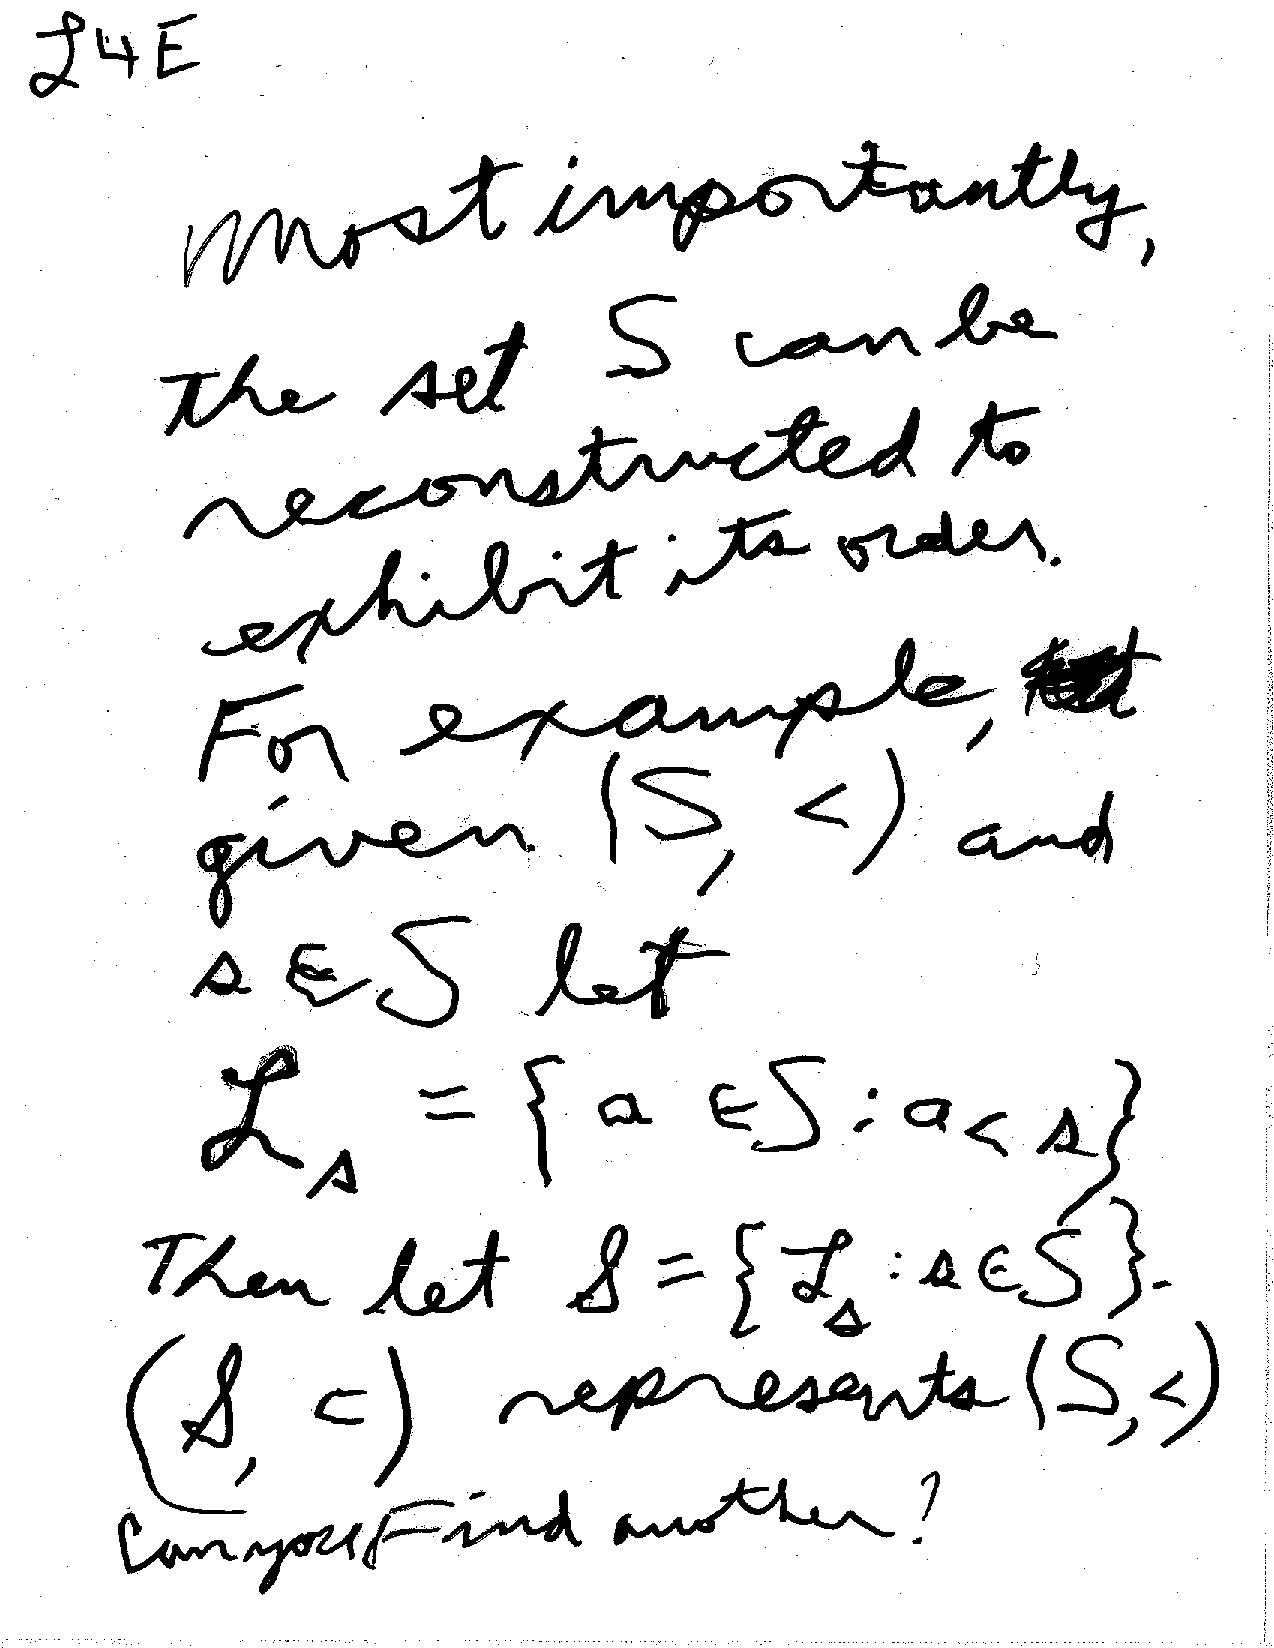
\includegraphics[scale=0.5]{Pages/generateN5.pdf}

\newpage

\begin{Large}
L4F Generate $\mathbb{N}$
\end{Large}

Given $\lbrace$ 1, 2, 3,... $\rbrace$ what do we do next? Ans: Fiddle with what we have. What is the 2nd successor of 1? 2? 3? etc. What is the 6th successor of n? These questions lead to the discovery of the operation of addition on $\mathbb{N}$. Since this operation is one-to-one it can (often) be inverted. Hence

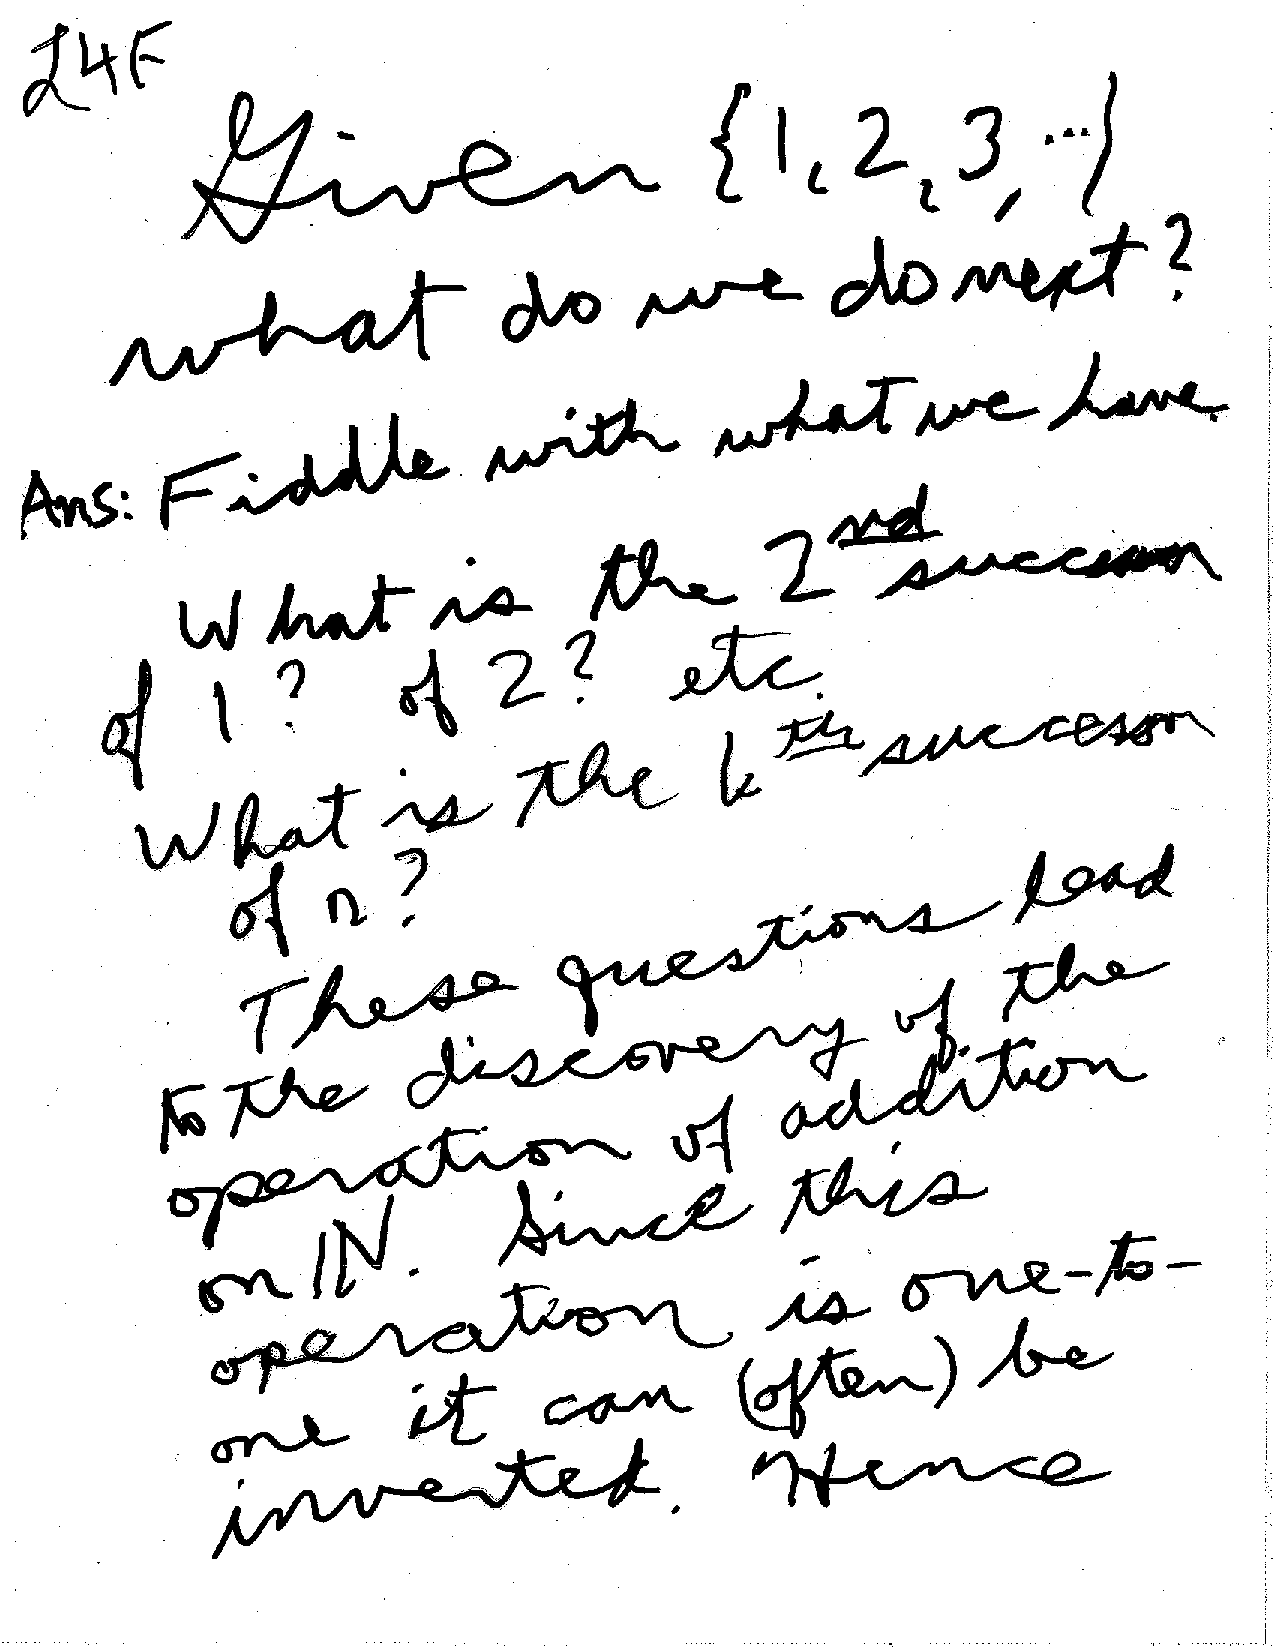
\includegraphics[scale=0.5]{Pages/generateN6.pdf}

\newpage

\begin{Large}
L4G Generate $\mathbb{N}$
\end{Large}

What is the 6th predecessor of n? Currently, this question can be answered if k $<$ n. We want to be able to answer it for all n and How? Necessarily we need numbers

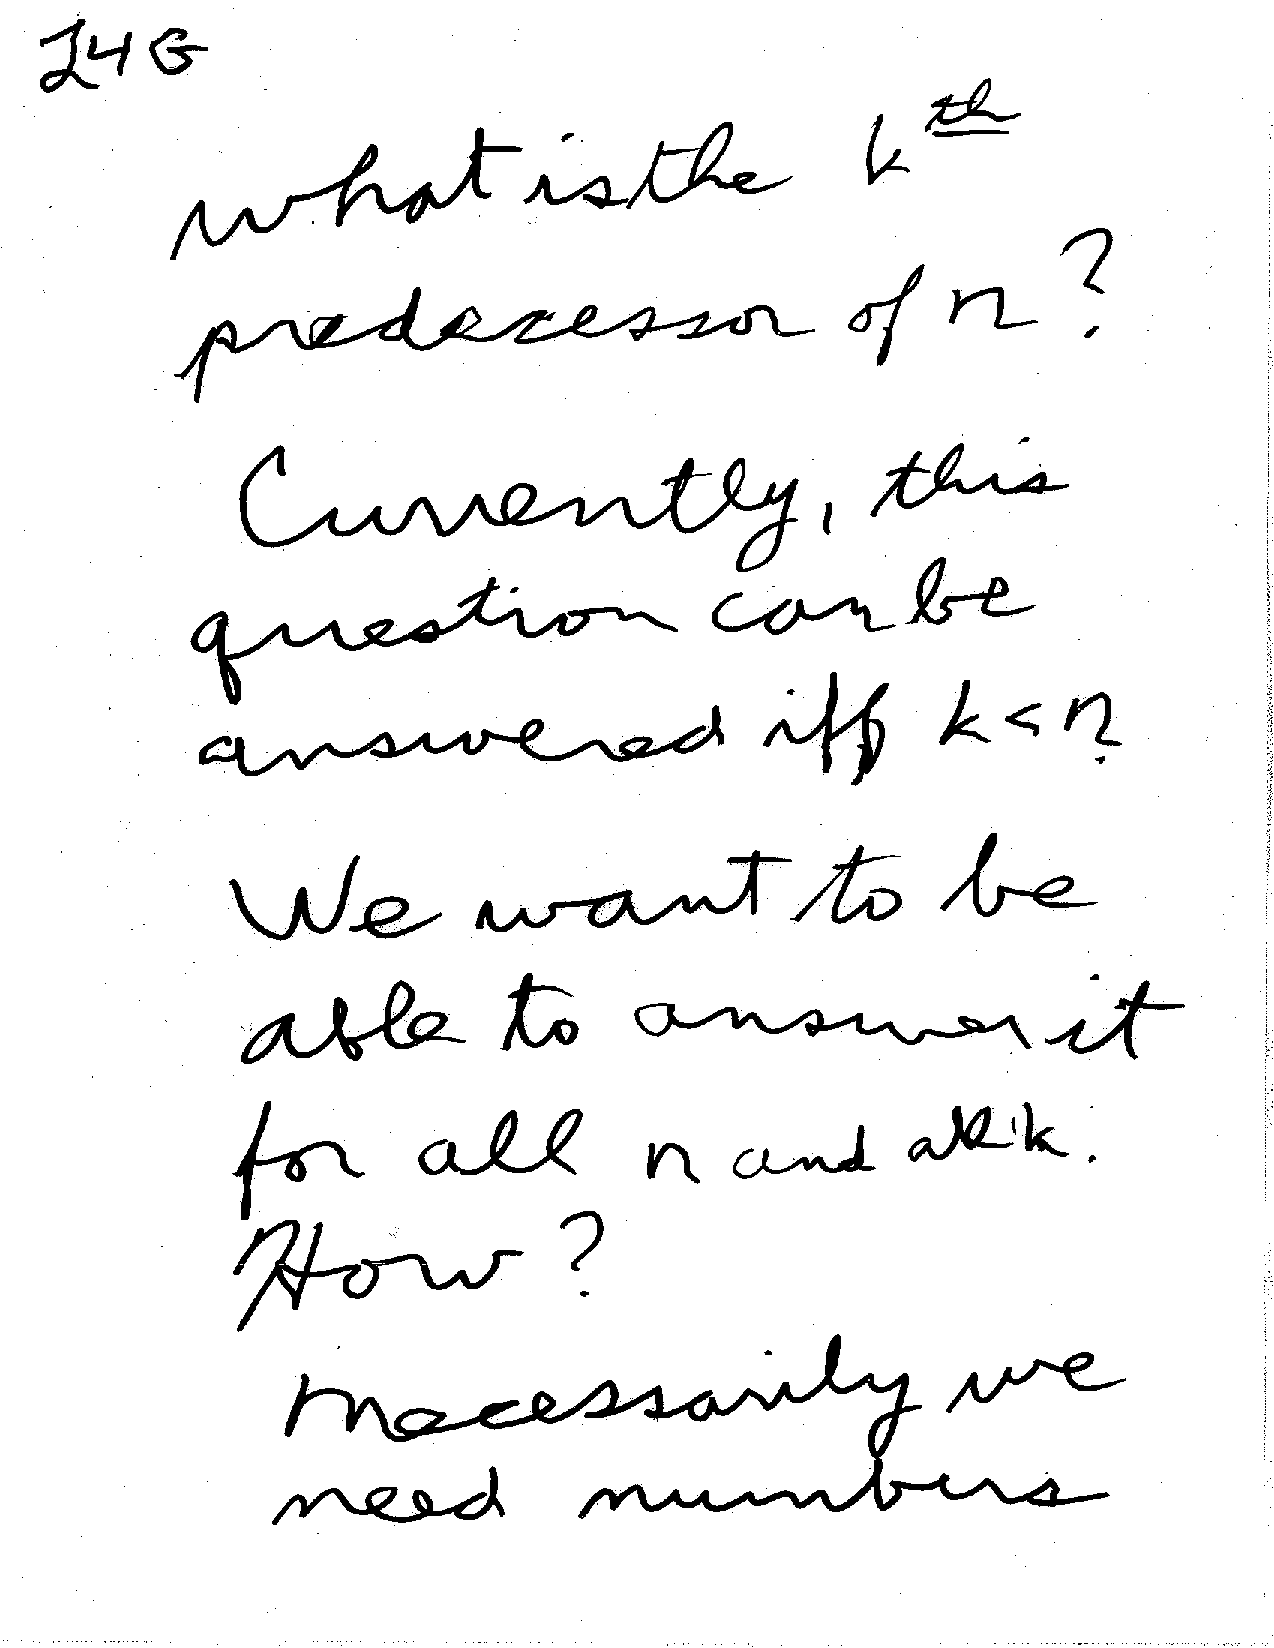
\includegraphics[scale=0.5]{Pages/generateN7.pdf}

\newpage


\newpage

\section{From $\mathbb{Z}$ to $\mathbb{R}$ via ordering}
%Jazz: ZR1-ZR5

\large
\underline{From Z to R via Orderings}\\

\normalsize

$\mathbb{Z}$ = {...,-1,0,1,...}\\We can put a strict ordering on it so that for all $n \in \mathbb{Z}$ , $n<n+1$.\\

With this ordering\\
	$0 \rightarrow 1$ in one step\\
	$0 \rightarrow 2$ in two successive step\\

Simplify for \\
	$n\rightarrow n+1$\\
	$n\rightarrow n+2$

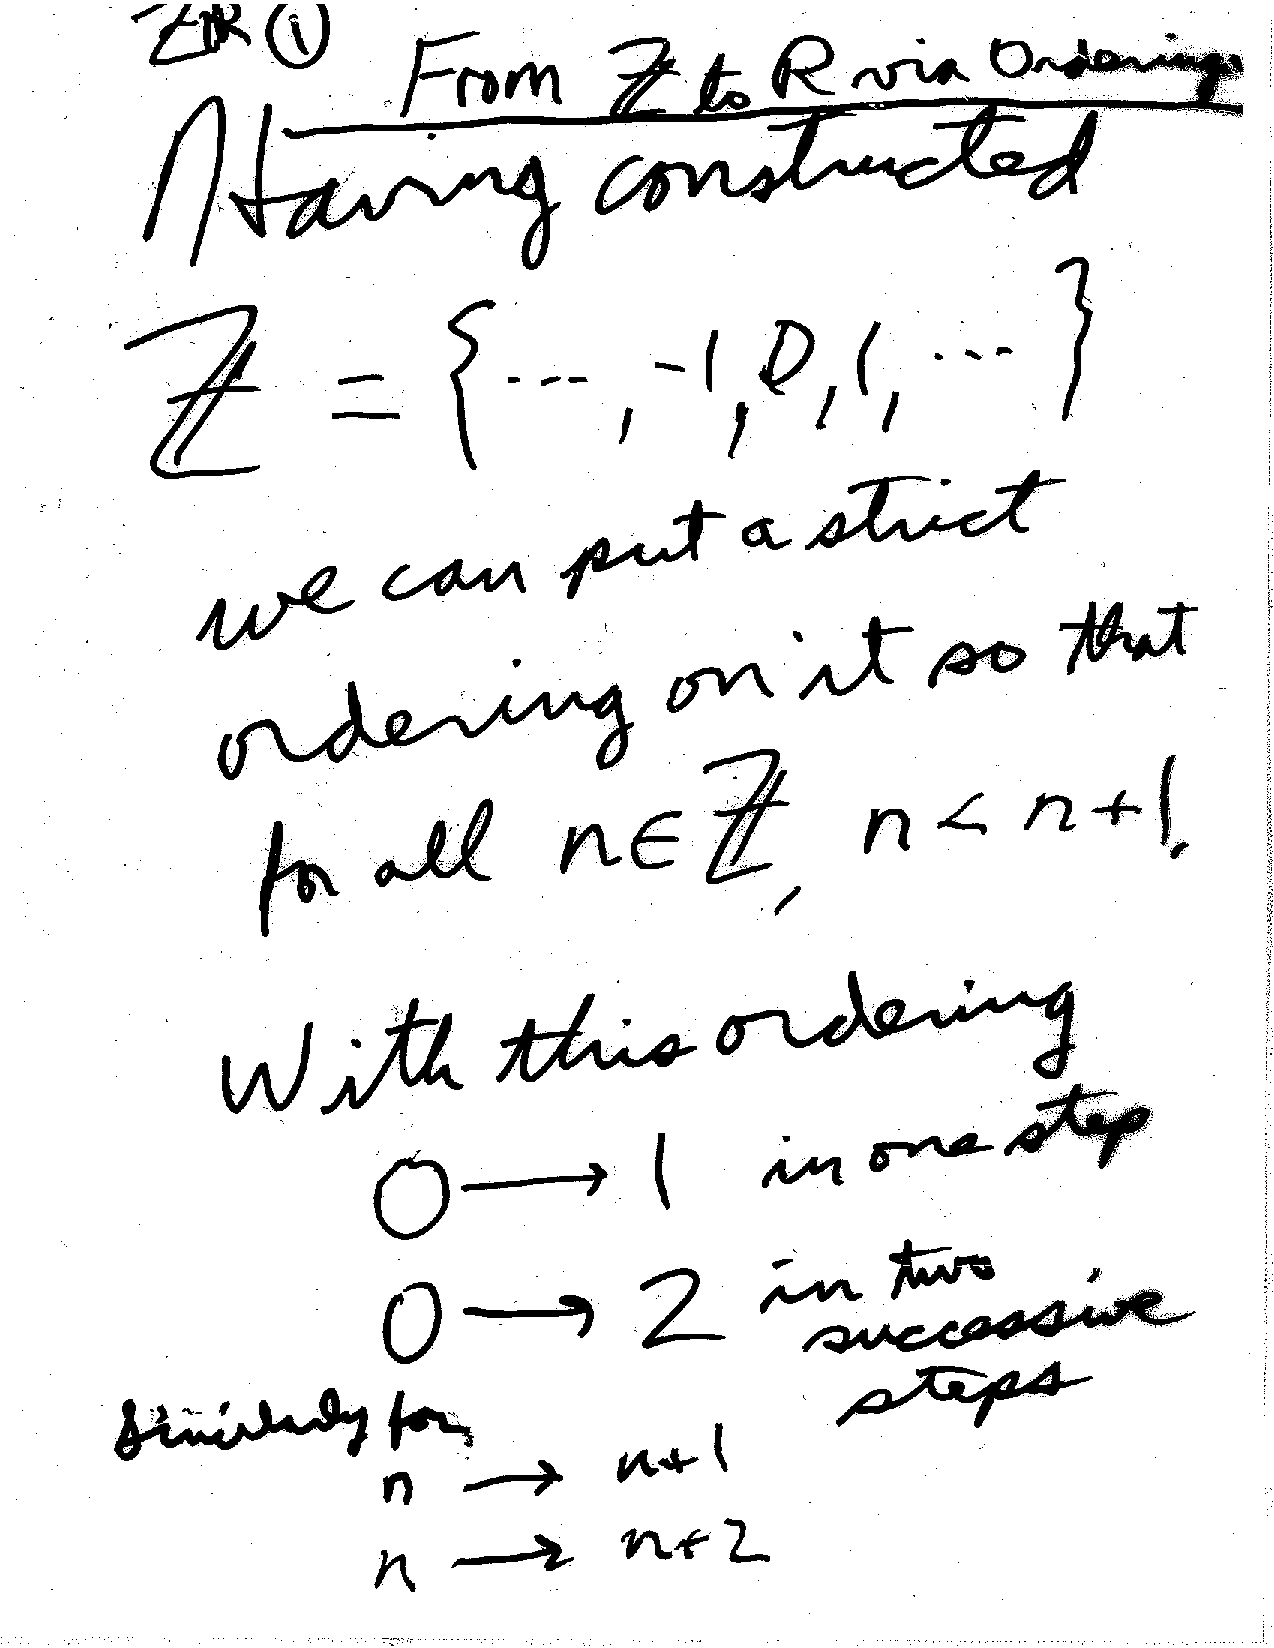
\includegraphics[scale=0.5]{Pages/ZR_1}

\newpage

Suppose we want to propose/construct the existence of a set\\
$\mathbb{Z}_{(2)}\neq \mathbb{Z}$\\
which requires two successive steps of some kind to go from\\
$0 \rightarrow 1$\\
and $n\rightarrow n+1$.\\
What is required?

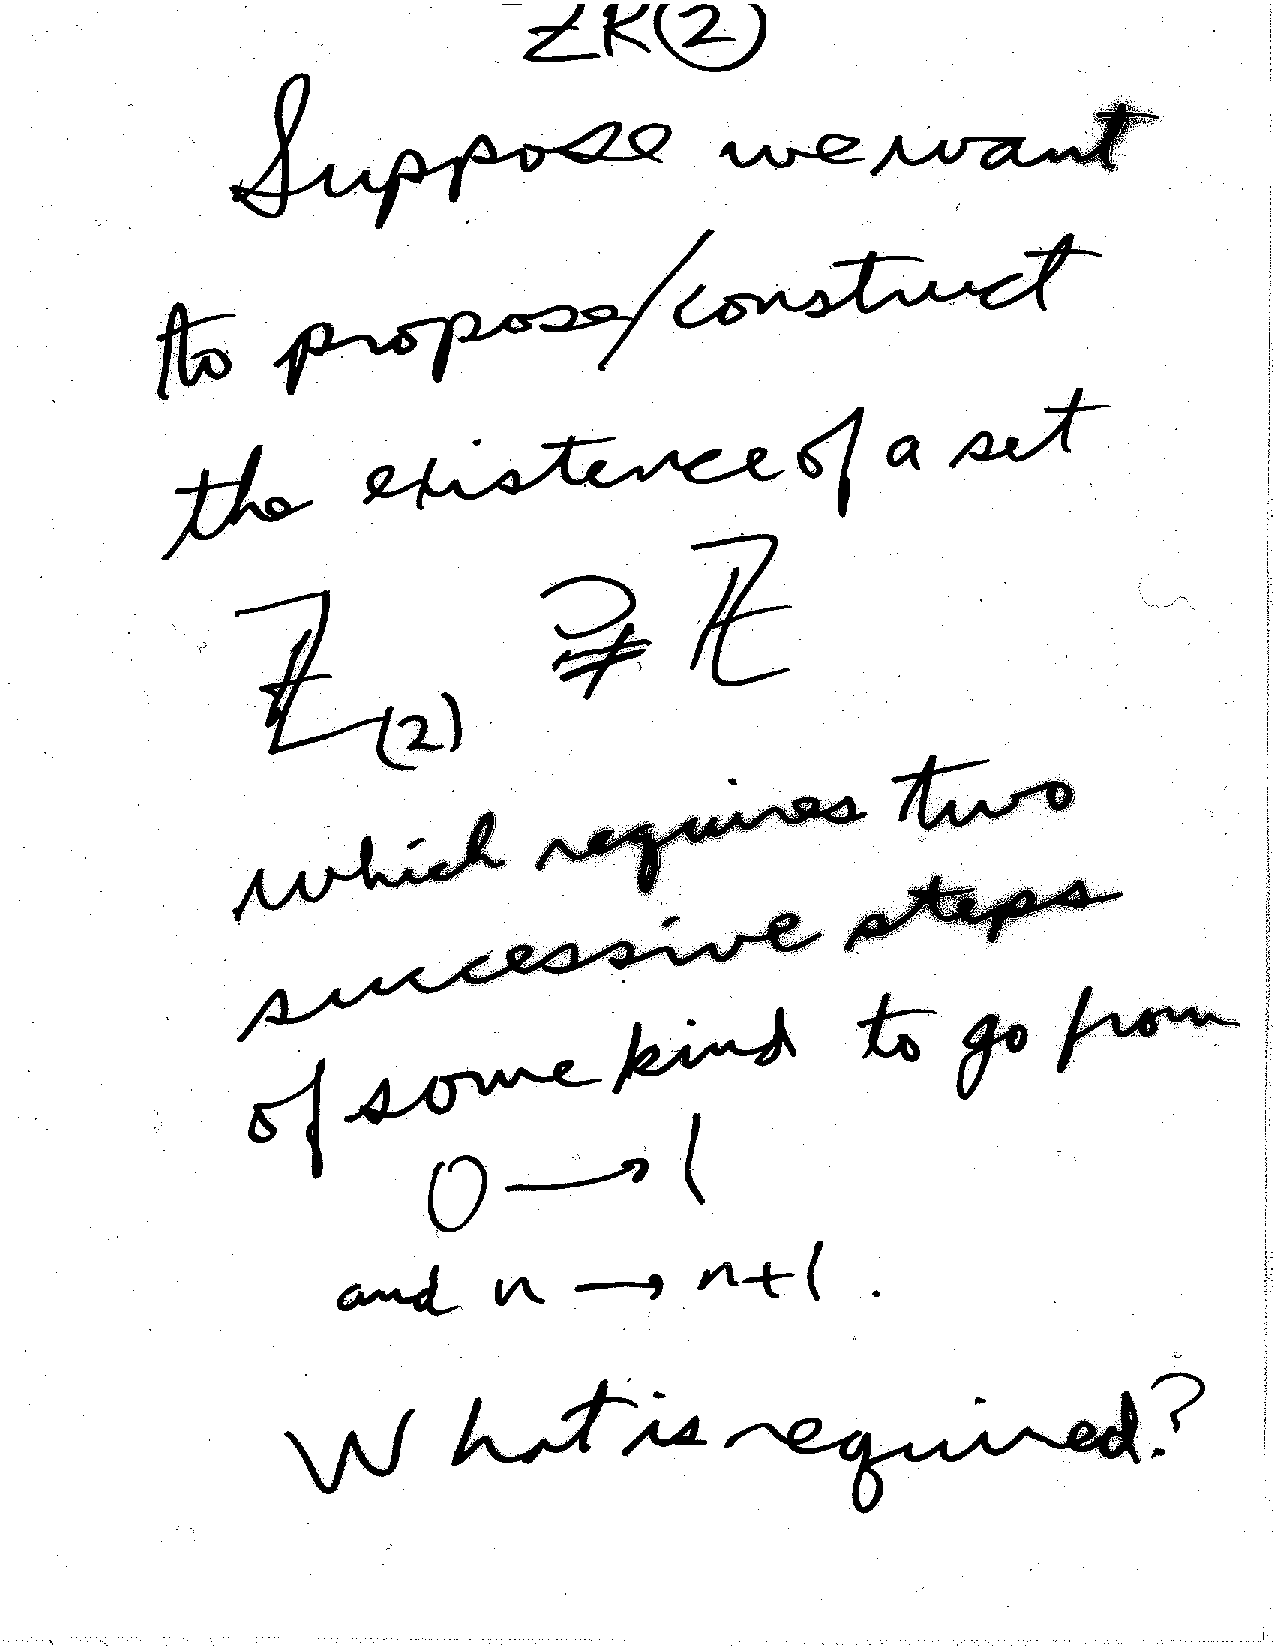
\includegraphics[scale=0.5]{Pages/ZR_2}

\newpage

We need to go from\\
$0\rightarrow x$ in one step and from $x\rightarrow1$ in the next\\
Similarly we go from $n\rightarrow n+x$ and $n+x$ to $n+1$.\\
We need a symbol to specify x. Let $x=\frac{1}{2}$.\\
Then $\mathbb{Z}_{(2)}=\mathbb{Z}\bigcup$\{$\in+\frac{1}{2}:n\in{Z}$\\
We can put an...

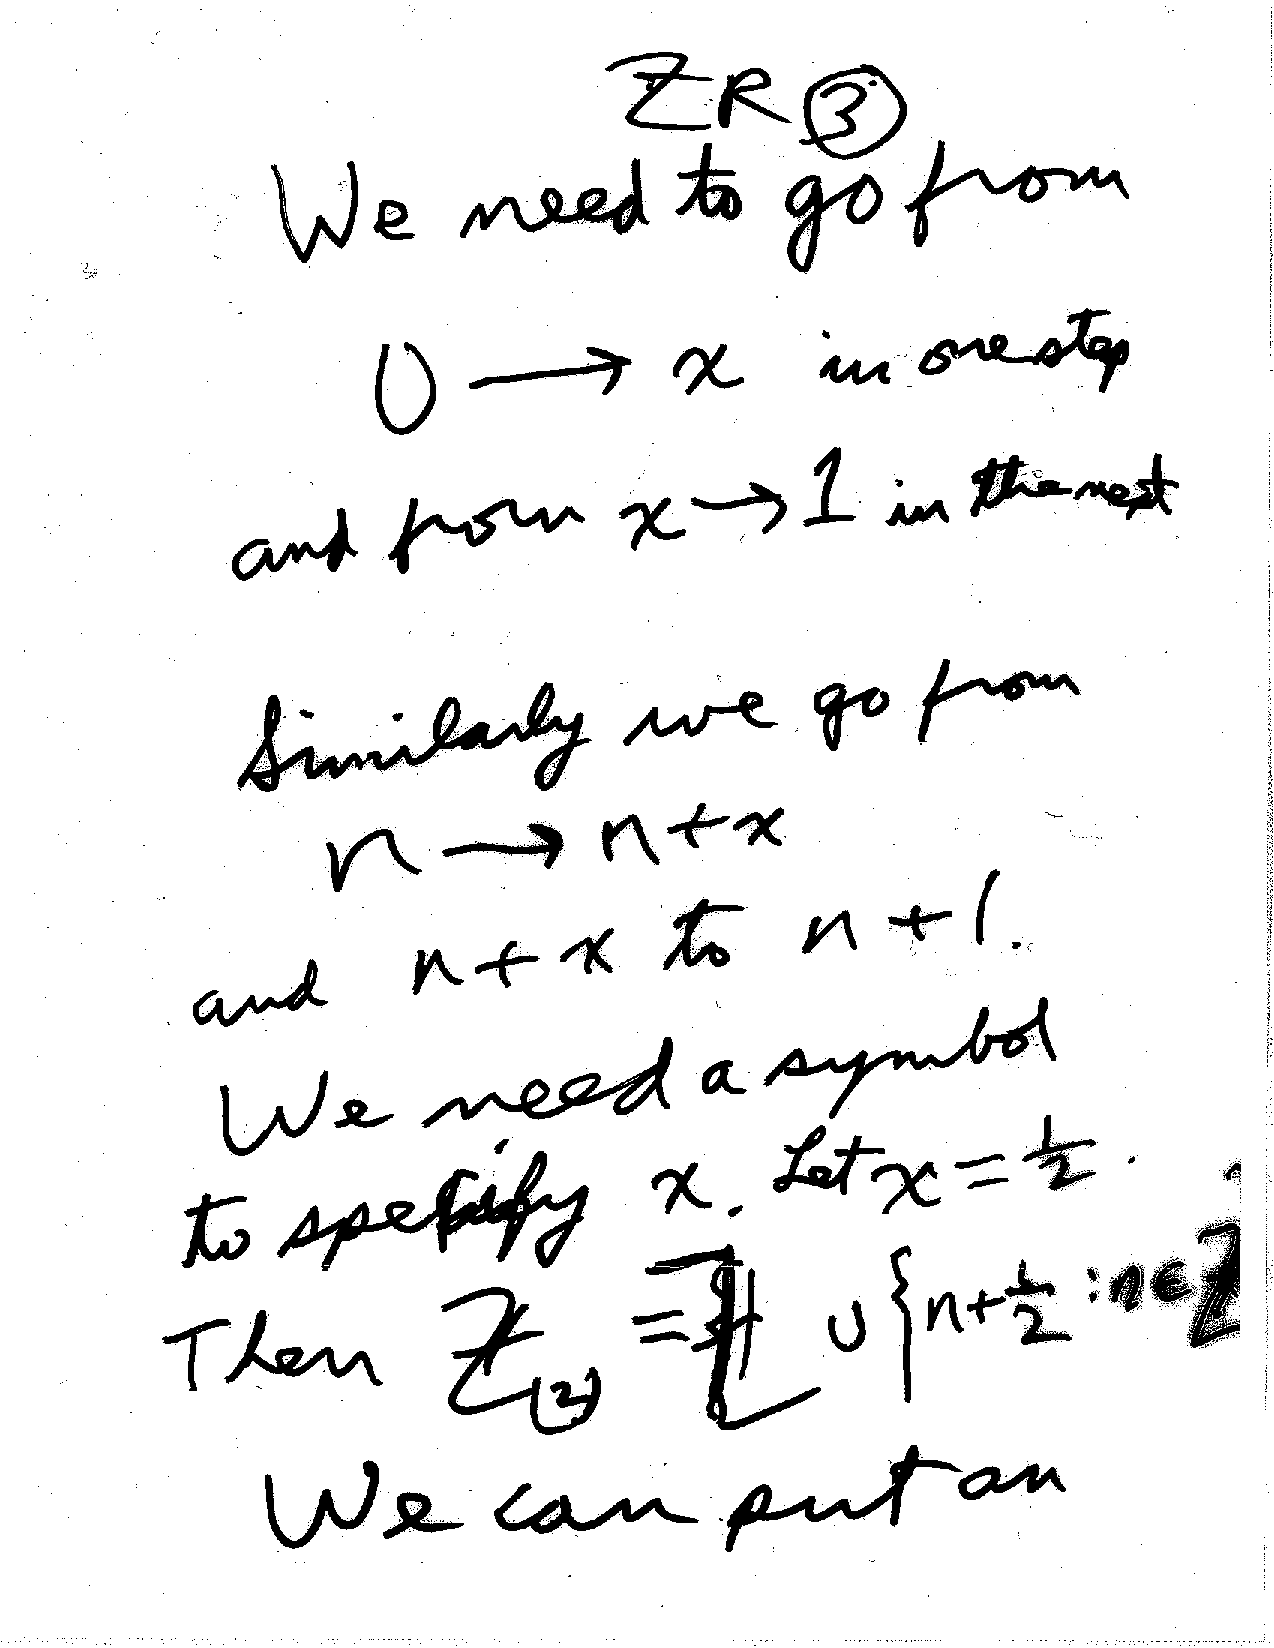
\includegraphics[scale=0.5]{Pages/ZR_3}

$\{$

\newpage

...ordering $<_{(2)}$ on $Z_{(2)}$ that \underline{extends} the ordering $<$ on $Z$. \\ 
\underline{Problem:} Let $(\mathcal{S};, <;)$ be two ordered sets such that $\mathcal{S}, \subseteq \mathcal{S}_2$.\\
\underline{Define} what it means to say that the ordering $<_{2}$ extends $<,$.\\

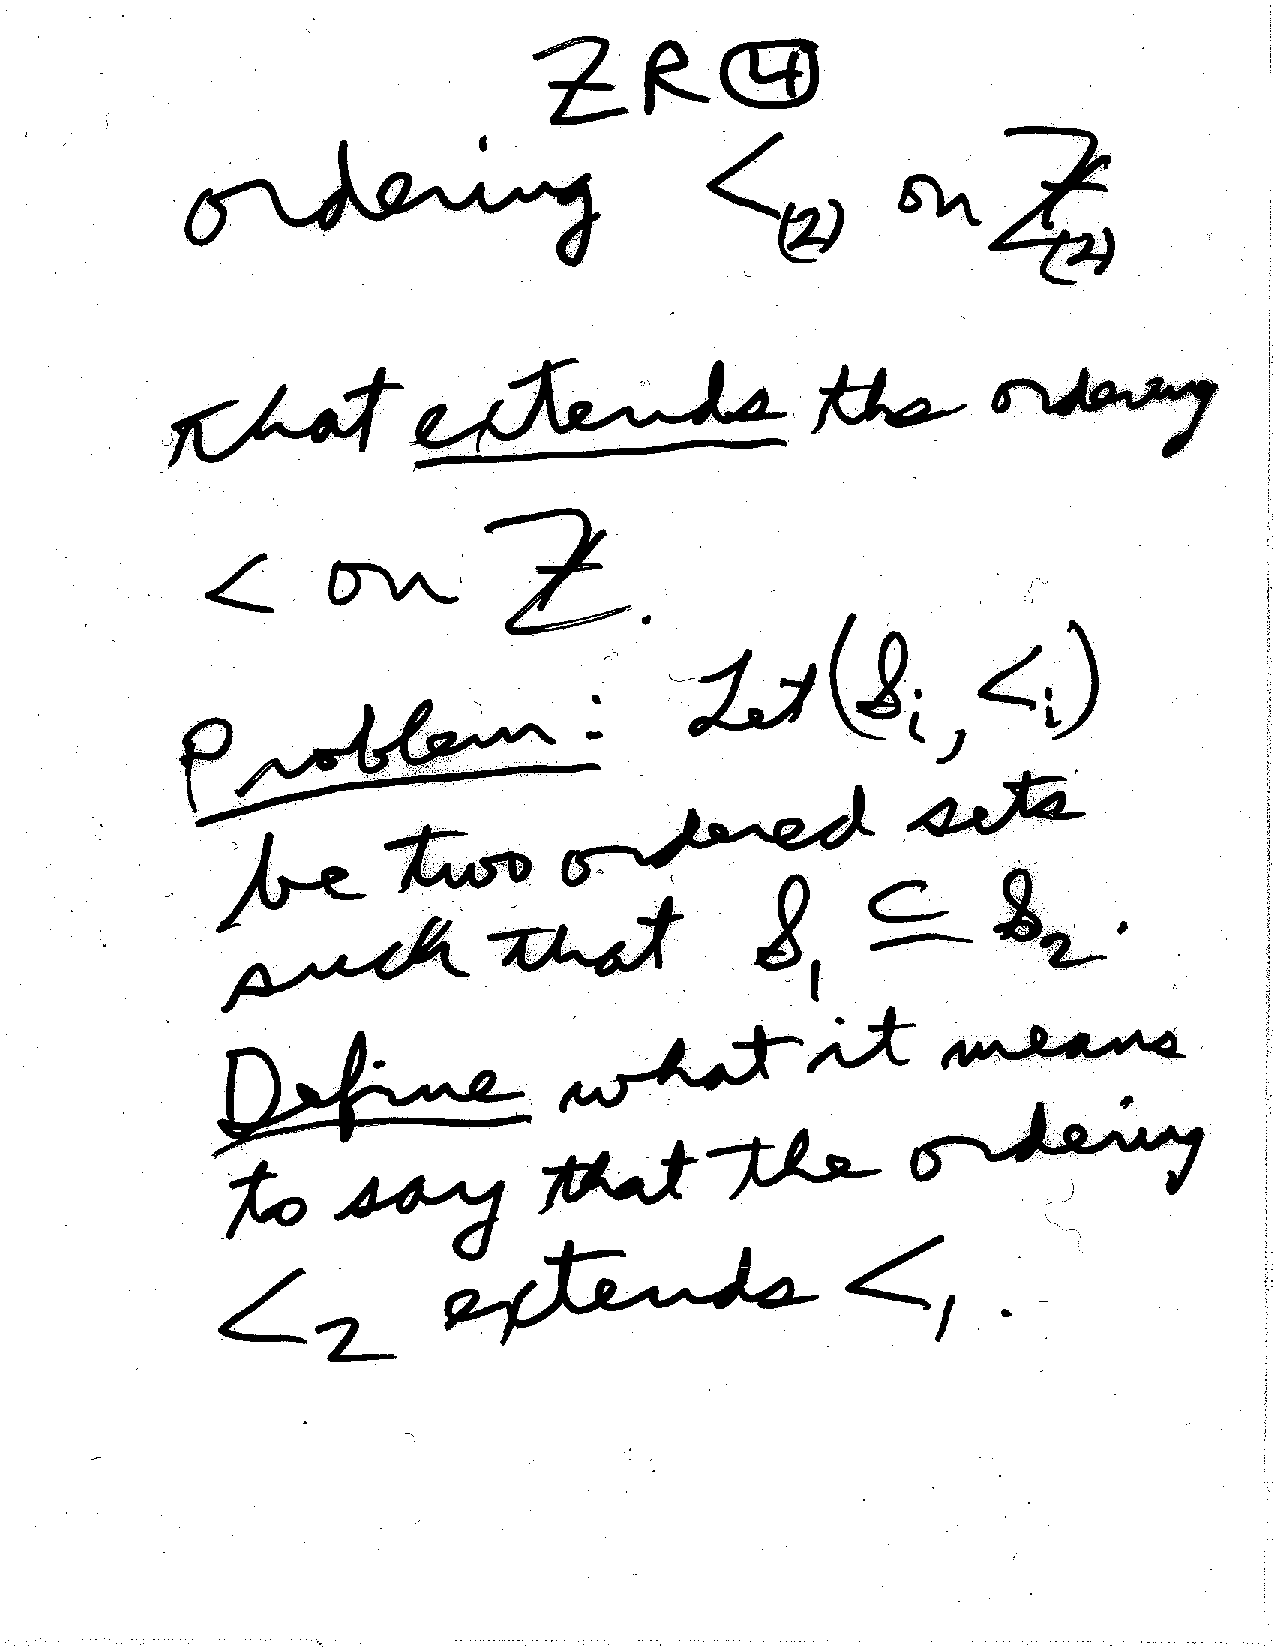
\includegraphics[scale=0.5]{Pages/ZR_4}

\newpage

For $Z_{(2)}$ there is a unique ordering $<_{(2)}$ such that\\
$n<_{(2)} n+\frac{1}{2}$ and $n+\frac{1}{2} <_{(2)} n+1$\\
Similarly, we can generate the ordered set $(Z_{(4)}, <_{4})$ where $Z_{(2)}$  sign  $Z_{(4)}$ and $<_{4}$ extends $<_{2}$

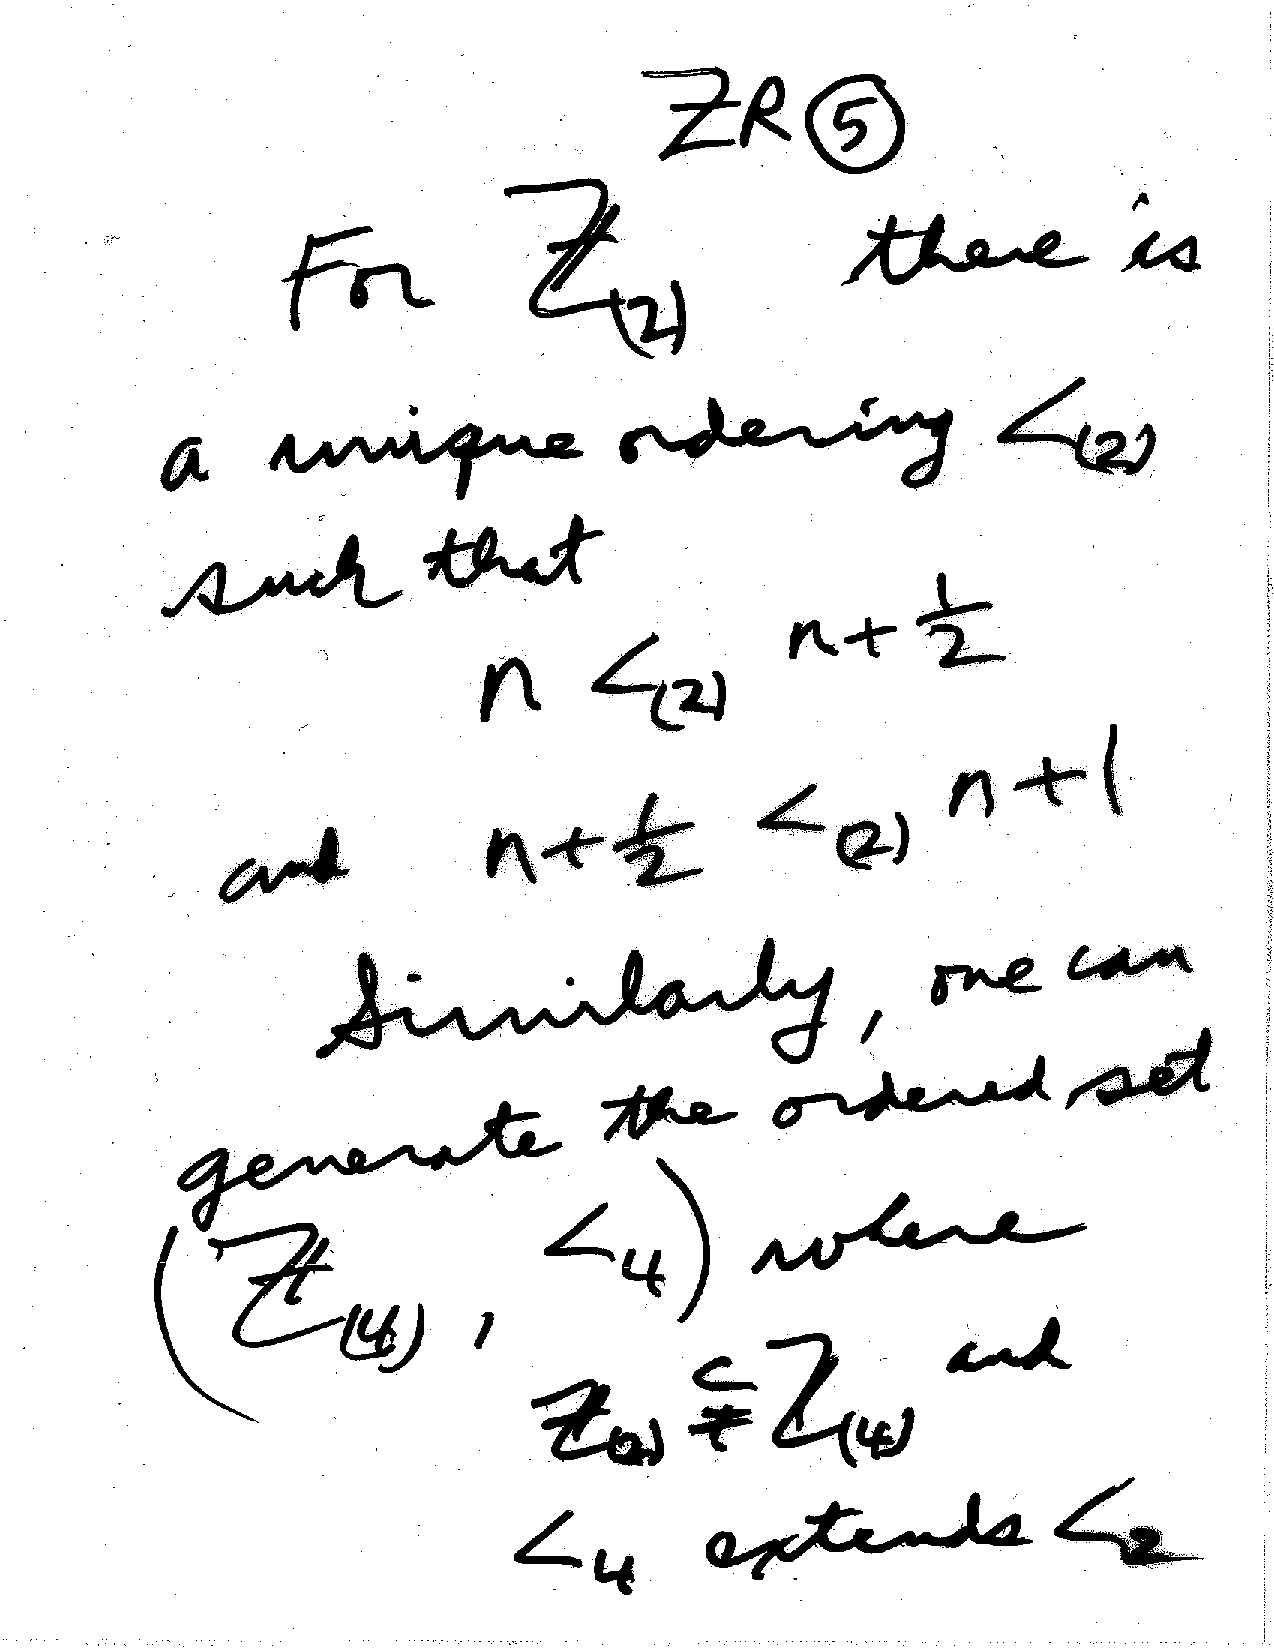
\includegraphics[scale=0.5]{Pages/ZR_5}

%Kyler: ZR6 - ZR10

ZR6

 
Continuing in this way we generate 

$(\mathbb{Z}_{2^k},<2_{2^k})$ For all $k\in\mathbb{N}$
                     


Then we get 

\quad\quad\quad$\infty$
           
$\mathbb{Z}_{\infty} = \bigcup$ $Z_{(2k)}$ 

  \quad\quad $k=1$

Problem: How do we put an ordering $<_{\infty}$ on $Z_{(\infty)}$ 

That extends every $<_{2k}$?

\quad
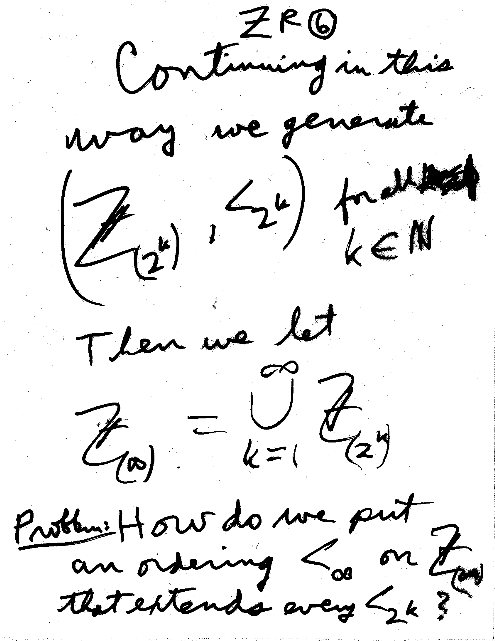
\includegraphics[scale=0.6]{Pages/ZR6.png}

\newpage 
\title{ZR7}
\maketitle

We can represent $\mathbb{Z}$ in terms of integers $j,k,n$ and that $\mathbb{Z} _{\infty} = \mathbb{Z}\bigcup$ $\left\{n+\frac{j}{2k} = k\geqslant1 and \lneqq j < z^k\right\}$

What does the ordering look like? 

Suppose we want to construct a version of $\mathbb{Z}_{(\infty)}$ that exhibits.  

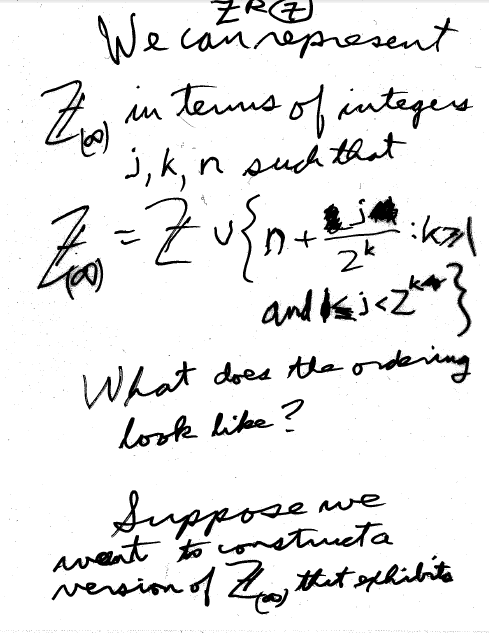
\includegraphics[scale=0.6]{Pages/ZR7.png} 

\newpage 

\title{ZR8}

\maketitle 

The ordering. 
for $x\in \mathbb{Z}_{\infty}$ let 

$L_{x}=\left\{y\in\mathbb{Z}:y<_{\infty}x\right\}$

Now $L_{x}$ denotes the dyadic rational x. 

notice that for any 

$x,y$ in $\mathbb{Z}_{\infty},$ 

$L_{x} \bigcup L_{y} = L_{w}$ for 

$w=x$ or $w=0$ 

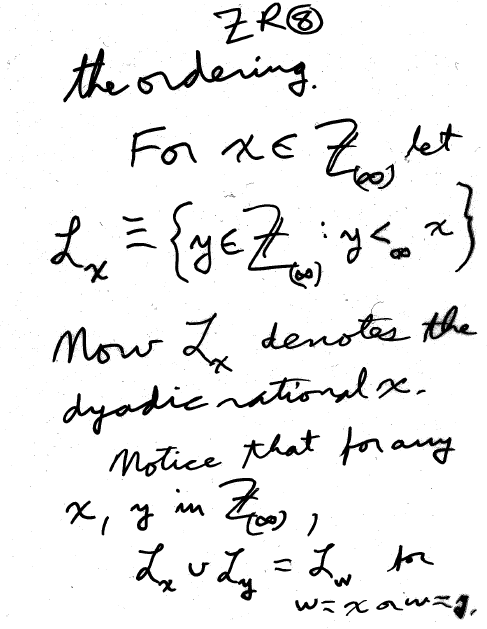
\includegraphics[scale=0.6]{pages/ZR8.png}

\newpage

\title{ZR9} 

\maketitle

Hence for any $n\geqslant1$ and $x,..., x_{n} \in \mathbb{Z}_{\infty}$
  


    $\bigcup_{j=1}^{n} L_{x_j} = L_{w}$ 
   
                          
               
      
       For w $\in$ $\bigcup_{j=1}^{n}$ $\left\{x_{j}\right\}$
                         
                          
               
Hence, finite unions of dyadic rationals one dyadic rationals suppose we want to think of arbitrary unions of 
$L{x}= x\in\mathbb{Z}_{\infty}$ as bone fide numbers. 

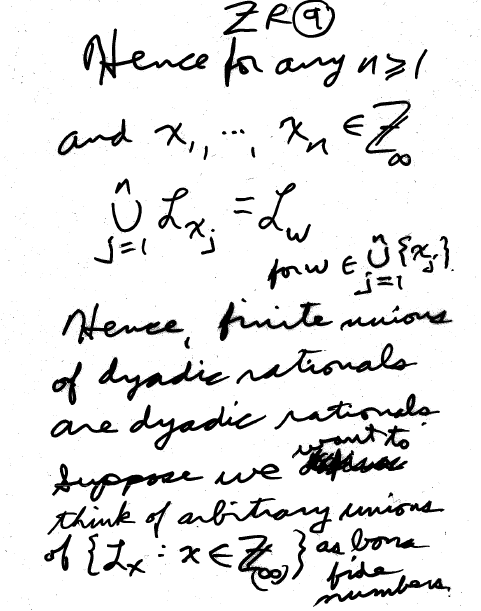
\includegraphics[scale=0.6]{pages/ZR9.png}

\newpage

ZR10



LET 

$R_{\infty}$ = $\left\{\bigcup_{X\in A} L_{x} = a\subseteq\mathbb{Z}_{\infty}\right\}$
         
            

Letting $A=\emptyset, \emptyset\in R_{\infty}$ 

Letting $A=\mathbb{N}, \mathbb{Z}_{\infty}\in R_{\infty}$

Let $R=\left\{B\in R_{\infty}:B\neq\emptyset \mbox{ and } B\neq\mathbb{Z}_{(\infty)}\right\}$  

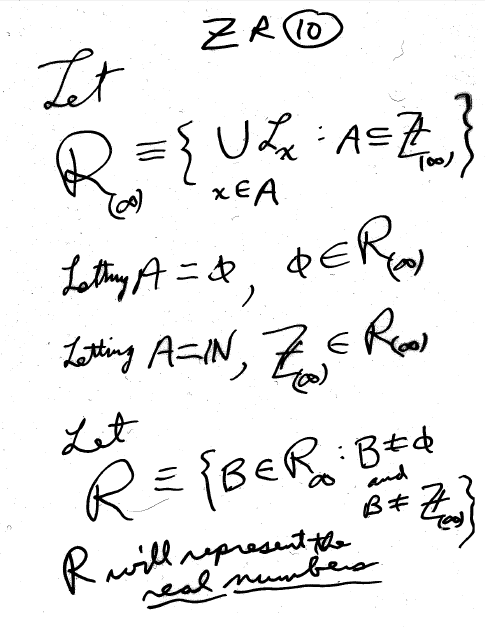
\includegraphics[scale=0.6]{pages/ZR10.png}

R will represent real numbers 
%Preethika: ZR11-ZR14
What do the elements of $\mathbb{R}$ look like? 
\\On the number line they look like

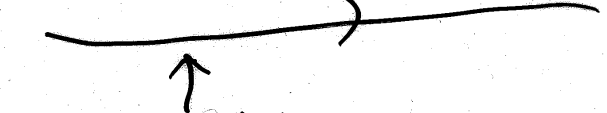
\includegraphics[scale=.5]{Pages/ZR_11_im1}
\\This set of dynamic rationals
\\How can we characterize them?

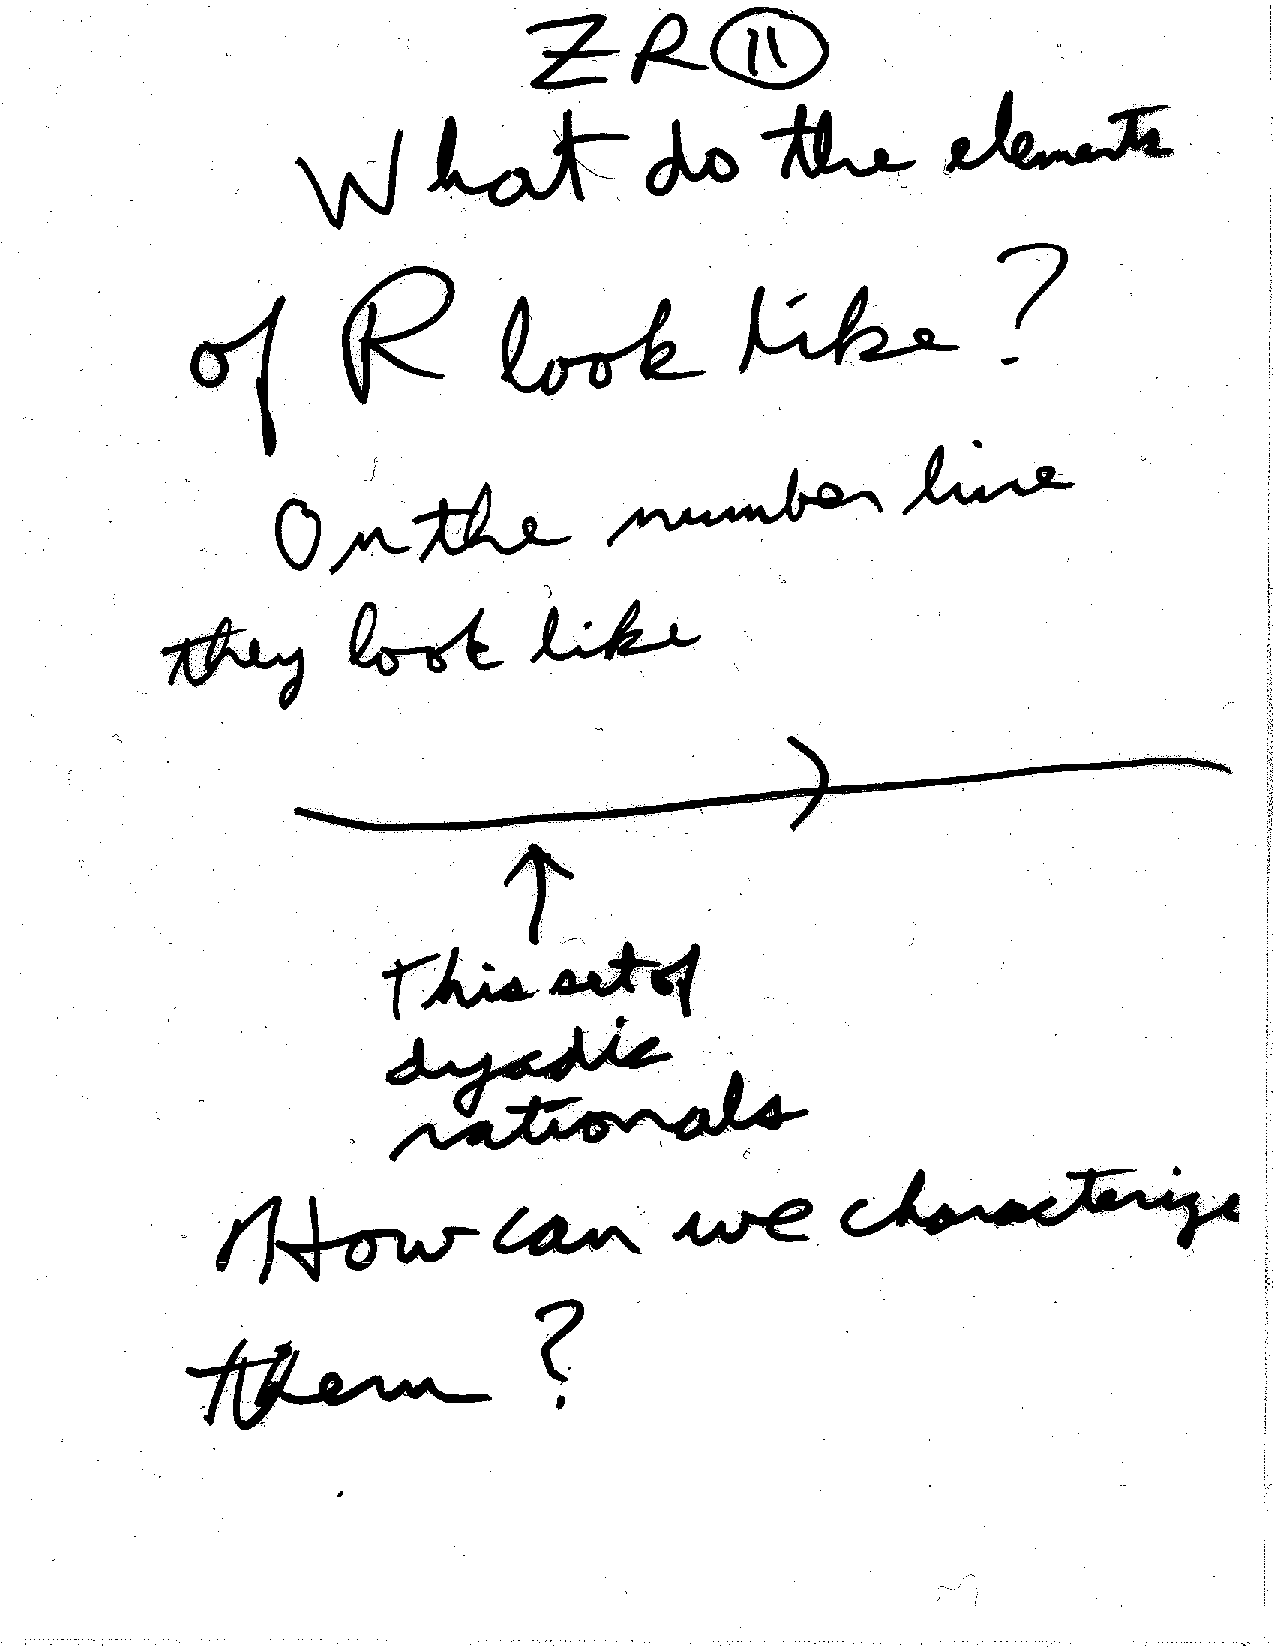
\includegraphics[scale=.5]{Pages/ZR_11}

\newpage

\underline{Therom} $B \in \mathbb{R}$ iff
\begin{enumerate}[(i)] 
\item $\phi \subsetneq B \subsetneq \mathbb{Z}_{(\infty)}$ 
\item If $b \in B$ and $a \in \mathbb{Z}_{(\infty)}$ with $a <_\infty b$ then $a \in B$
\item If $b \in B$ 
\\ $\exists b' \in B$ s.t
\\ $b <_\infty b'$

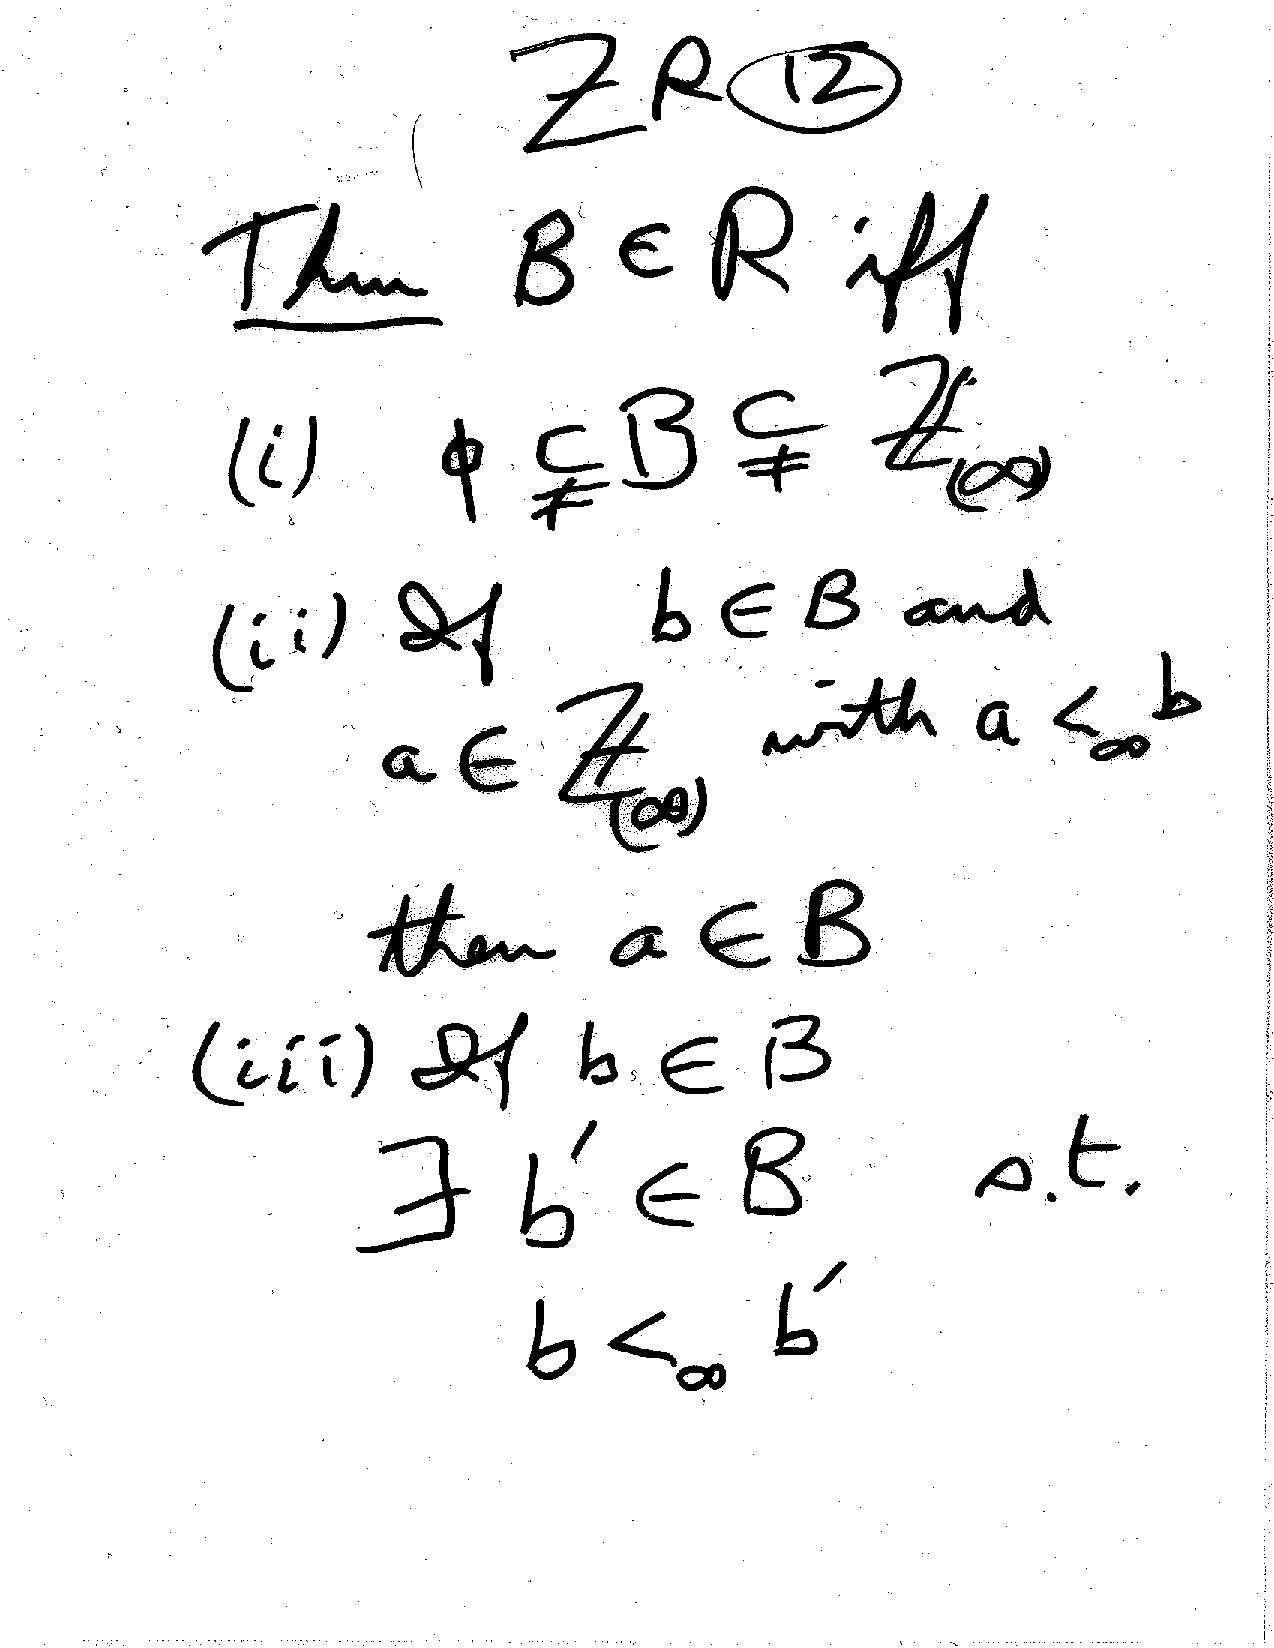
\includegraphics[scale=.5]{Pages/ZR_12}
\end{enumerate}

\newpage

$\underline{Pf:}^{(\Rightarrow)}$ Spse $B \in \mathbb{R}$
\\ $\exists$ non-entry $A \underline{\subset} \mathbb{Z}_{(\infty)}$
\\ s.t $$B=\bigcup_{a \in A} \mathcal{L}_a$$
\\ We are given that
\\ $B \neq \emptyset$ and $B \neq \mathbb{Z}_{(\infty)}$ 
\begin{enumerate}[(ii)] 
\item Spse $b \in B$
\\ and $b_o <_\infty b$ with $b_o \in \mathbb{Z}_{(\infty)}$
\\ $\exists a \in A: b \in \mathcal{L}_a$
\\hence $b_o \in \mathcal{L}_a$
\\ so $b_o \in B$
\item holds for -------$>$ $\mathcal{L}_a$ so (iii) holds. 

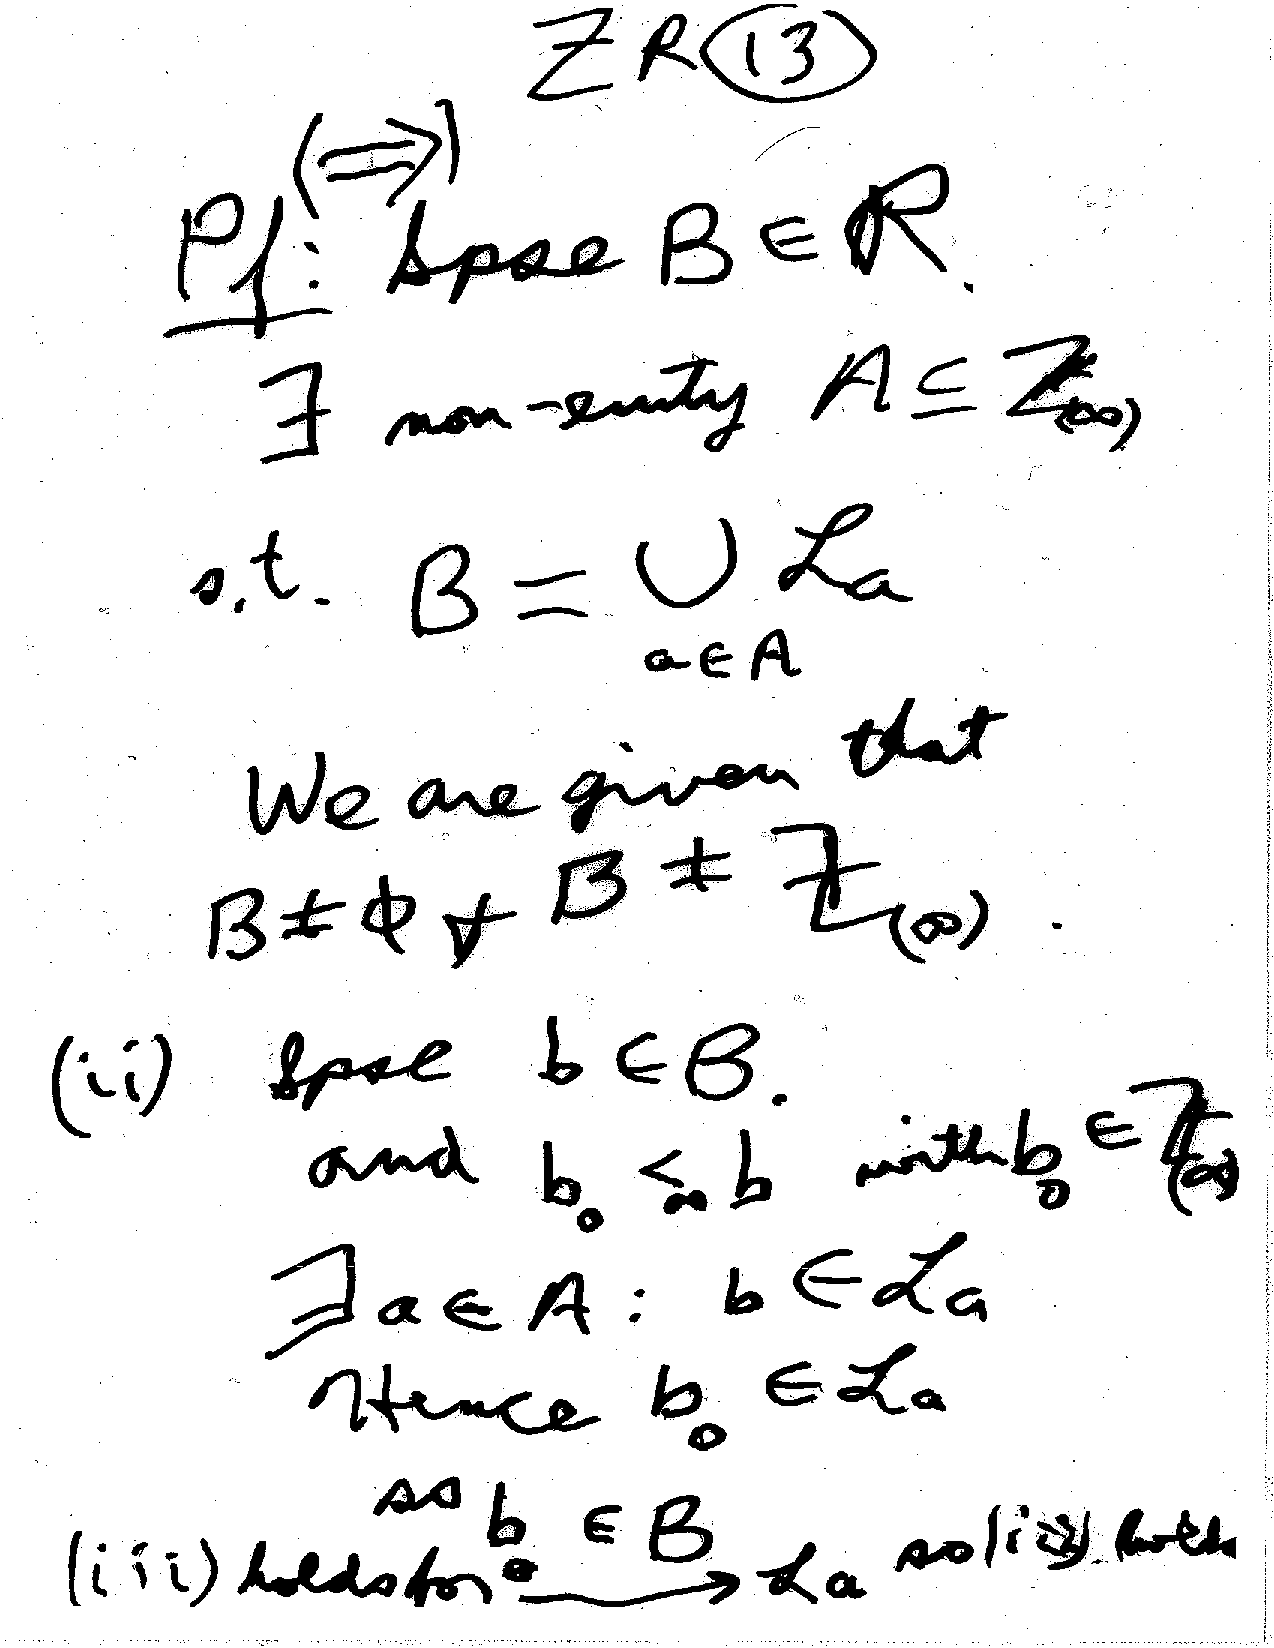
\includegraphics[scale=.5]{Pages/ZR_13}

\newpage
($\Leftarrow$)Conversely,
\\Spse B satisfies (i),(ii),(iii)
\\Let $A=B$
\\$\emptyset \subsetneq A \subsetneq \mathbb{Z}_{(\infty)}$
\\Claim $$B=\bigcup_{a \in A} \mathcal{L}_a $$ 
\\Clearly $ \bigcup \mathcal{L}_a \underline{\subset} B$ (Why?)
\\Take away $b \in B$. 
\\ $\exists b' >_\infty b$ s.t $b' \in B$
\\ $b \in \mathcal{L}_b{'}$ so
\\ $$B \underline{\subset} \bigcup_{a \in A} \mathcal{L}_a$$ qed

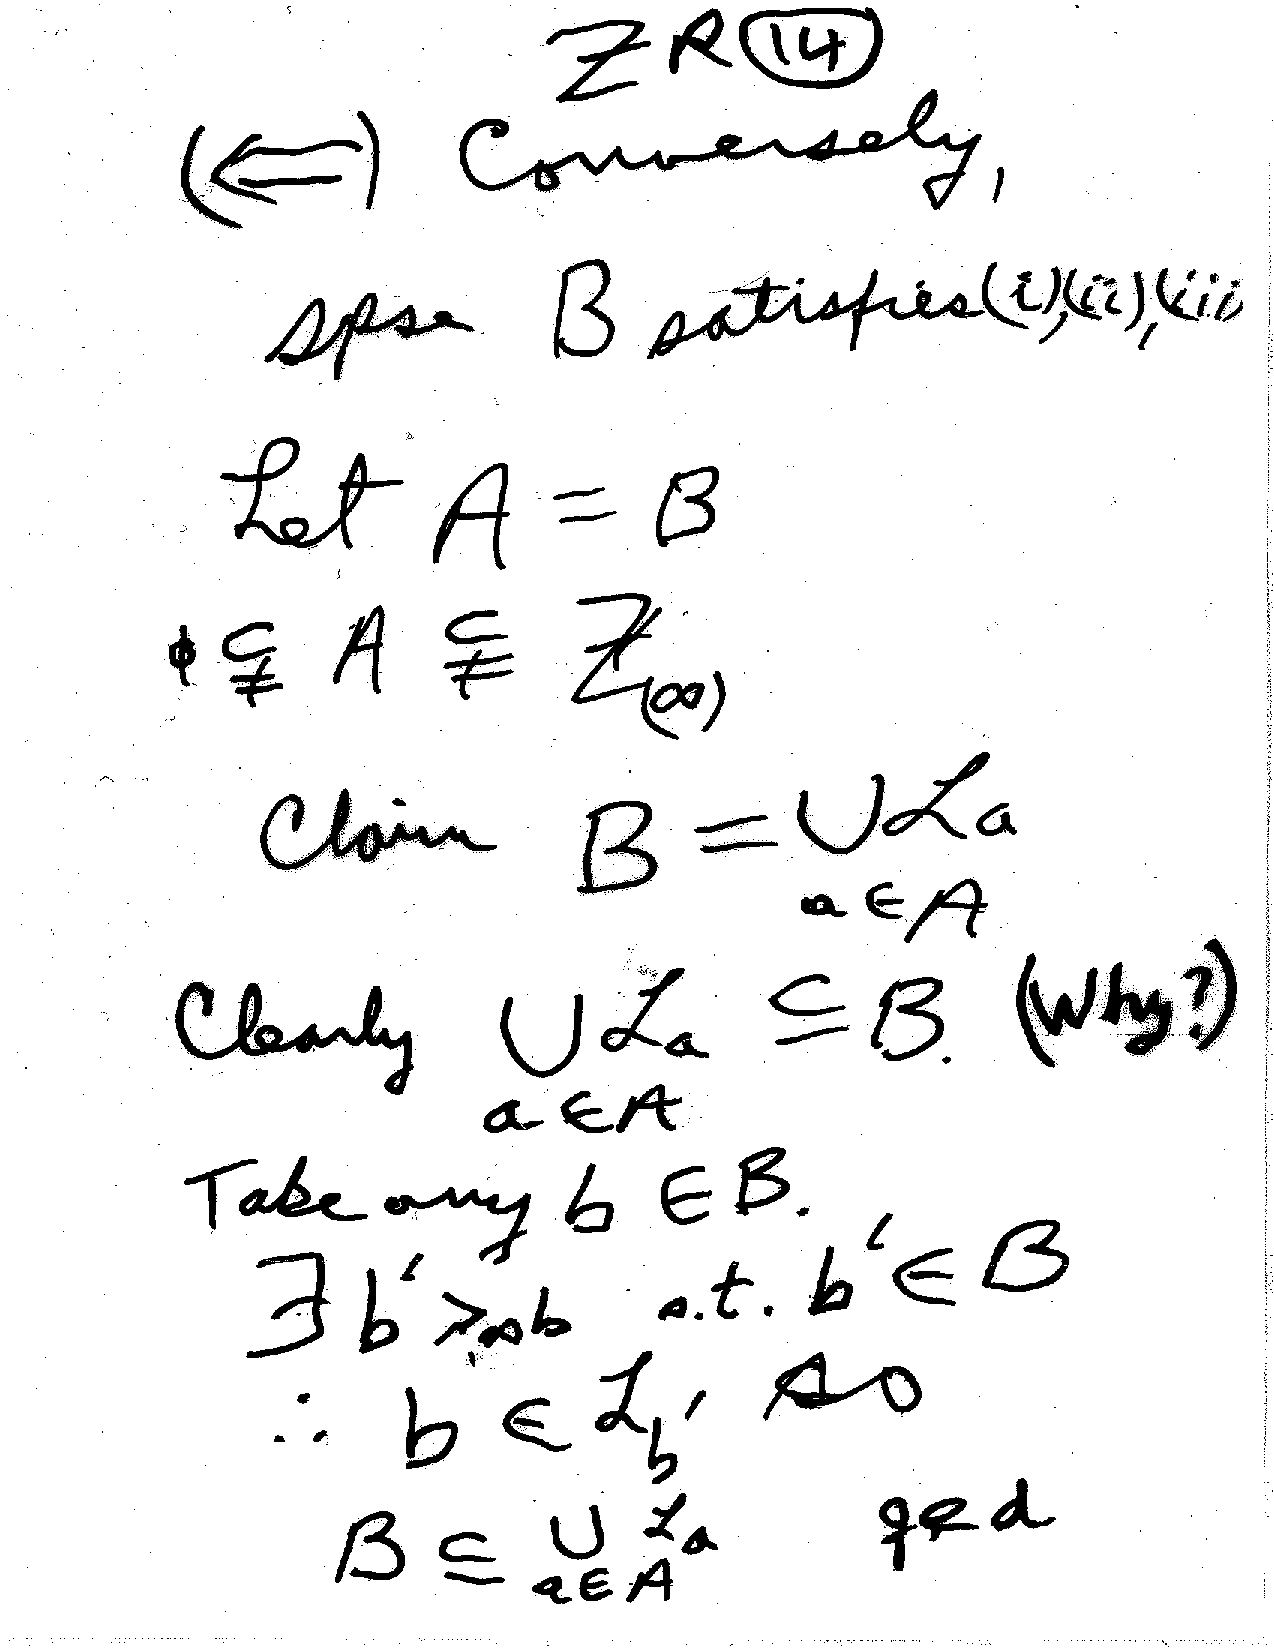
\includegraphics[scale=.5]{Pages/ZR_14}

\end{enumerate}

\section{Sequence and Limits}

%Aaron: First 2 pages and 48-50

Sequences

Limits

Constructing the limit via:

\begin{enumerate} [(i)]

\item Monotonic Sequences
\item Monotonic Sub-sequences 

\end{enumerate}

Cauchy Sequences

Subsequential Limits 

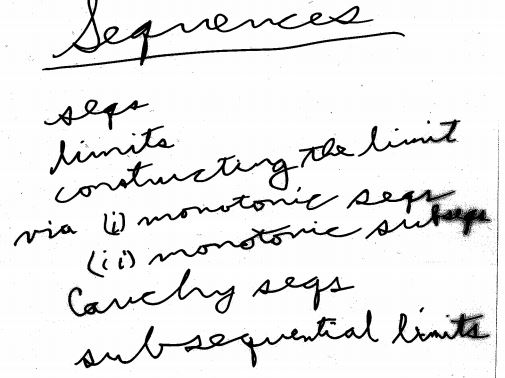
\includegraphics[scale=.8]{Pages/S&L_page1}

\newpage


Besides $\vec{a}$ = $(a{_0}, a_{1}, a_{2}, ...)$, how else might we harness elements of $\mathbb {R}^{2}$?

$$s_0 = a_{0}$$

$$s_1 = a_{0} + \frac{a_{1}}{2}$$



$$s_{n} = \sum_{j=0}^{n} a_{j} 2^{-j}$$




The sequence $\{s_{n}\}$ represents \{ ${z \in \mathbb{Z}_{\infty} : z < s_{n}} $ for all in sufficient large \}

It has a limit of $s_{\infty}$

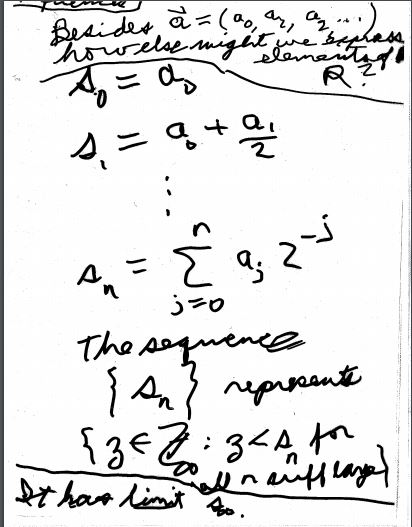
\includegraphics[scale=.8]{Pages/S&L_page2}

\newpage
{\bf Sequences}


Def: a sequence \{ ${a_n}_{1}^\infty$ \} is a map from the integers. A real valued sequence is a map into the reale from the integers.

Examples:

\begin{enumerate} [{}]

\item $a{_n}$ = $\frac{1}{n^{2}}$
\item $a_{n} = (-c)^{n}$
\item $a_{n} = \cos(nx)$
\item $a_{n} = n^\frac{1}{n}$
\item $a_{n} = (1 + \frac{1}{n})^{n}$

\end{enumerate}

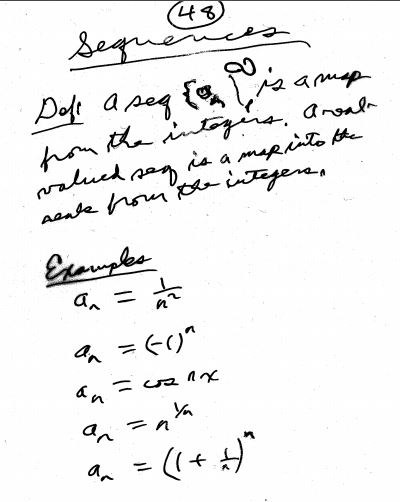
\includegraphics[scale=.8]{Pages/S&L_page48}

\newpage

{\bf Convergence of Sequences} 

Def: $a_{n} \rightarrow a$ if and only if $\forall \epsilon > 0\exists N$:

for all n $\geq N$, $|a_{n} - a| < \epsilon$

we write... $$a = \lim_{n \rightarrow \infty} a_{n}$$

Def: $a_{n} \rightarrow + \infty$ if and only if $\forall b < \infty$ $\epsilon N_{b}$ such that for all $n \geq , N_{b} , a_{n} \geq b$ 

Def: $a_{n} \rightarrow - \infty$ ?

Then (limits are unique)

if $a_{n} \rightarrow a$ and $a_{n} \rightarrow b$

then $a=b$

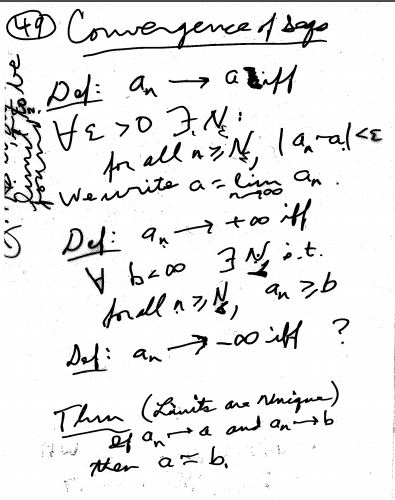
\includegraphics[scale=.8]{Pages/S&L_page49(1)}

\newpage

{\bf Convergence in $\mathbb {R}_{\infty}$ An Elegant Reformation}

Def: Let $\{ a_{n} \}$ be a sequence of reals and $a_{\infty} \epsilon \mathbb {R} \bigcup$ $\{  \pm \infty \}$ .

$\lim_{n \rightarrow \infty} a_{n} = a_{\infty}$ if and only if...

\begin{enumerate} [(i)]

\item $\forall$ real $b > a_{\infty}$

$\exists N_{b} < \infty$ : for all

$n \geq N_{b}$, $a_{n} < b$

\end{enumerate}

and

\begin{enumerate} [(ii)]

\item $\forall$ real $b < a_{\infty}$

$\exists N_{b} < \infty$: for all

$n \geq N_{b}$, $a_{n} > b$

\end{enumerate}

you prove

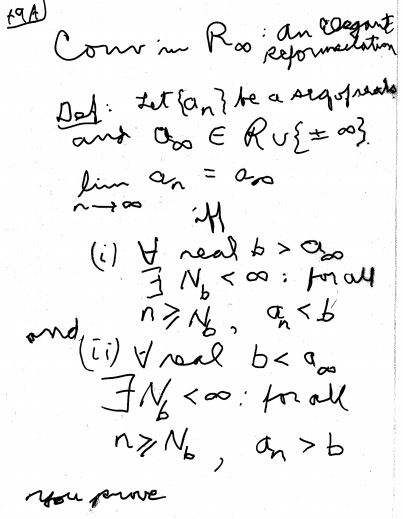
\includegraphics[scale=.7]{Pages/S&L_page49(2)}

\newpage


{\bf Finding Limits and Proving Convergence}

Example 1: $\lim_{n \rightarrow \infty} \frac{1}{n^{2}} = 0$

Example 2: $\lim_{n \rightarrow \infty} \frac{3n+1}{7n-4} = \frac{3}{7}$

Example 3: $\lim_{n \rightarrow \infty} (1 + \frac{1}{n})^{n} = e$

Homework: Suppose $a_{n} \rightarrow a > 0$


Prove $\sqrt{a_{n}} \rightarrow \sqrt{a}$

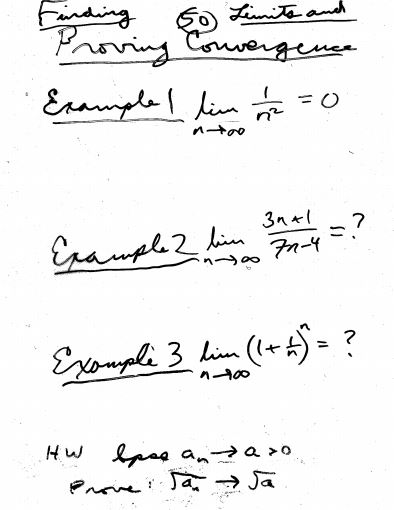
\includegraphics[scale=.7]{Pages/S&L_page50}

\newpage











%Hamza: 51-52B
{Theorem Suppose $a_n \rightarrow a$ and $b_n \rightarrow b$. Then $a_n + b_n \rightarrow a + b$ (and $ \lambda a_n \rightarrow	\lambda a$)and $a_n b_n \rightarrow a * b$}\newline

{Theorem if $a_n \rightarrow a \neq 0$, then $\frac{1}{a_n} \rightarrow \frac{1}{a}$}\newline

{corollary if $a_n \rightarrow a$ and $b_n \rightarrow b \neq 0$ then $\frac{a_n}{b_n} \rightarrow \frac{a}{b}$} \newline

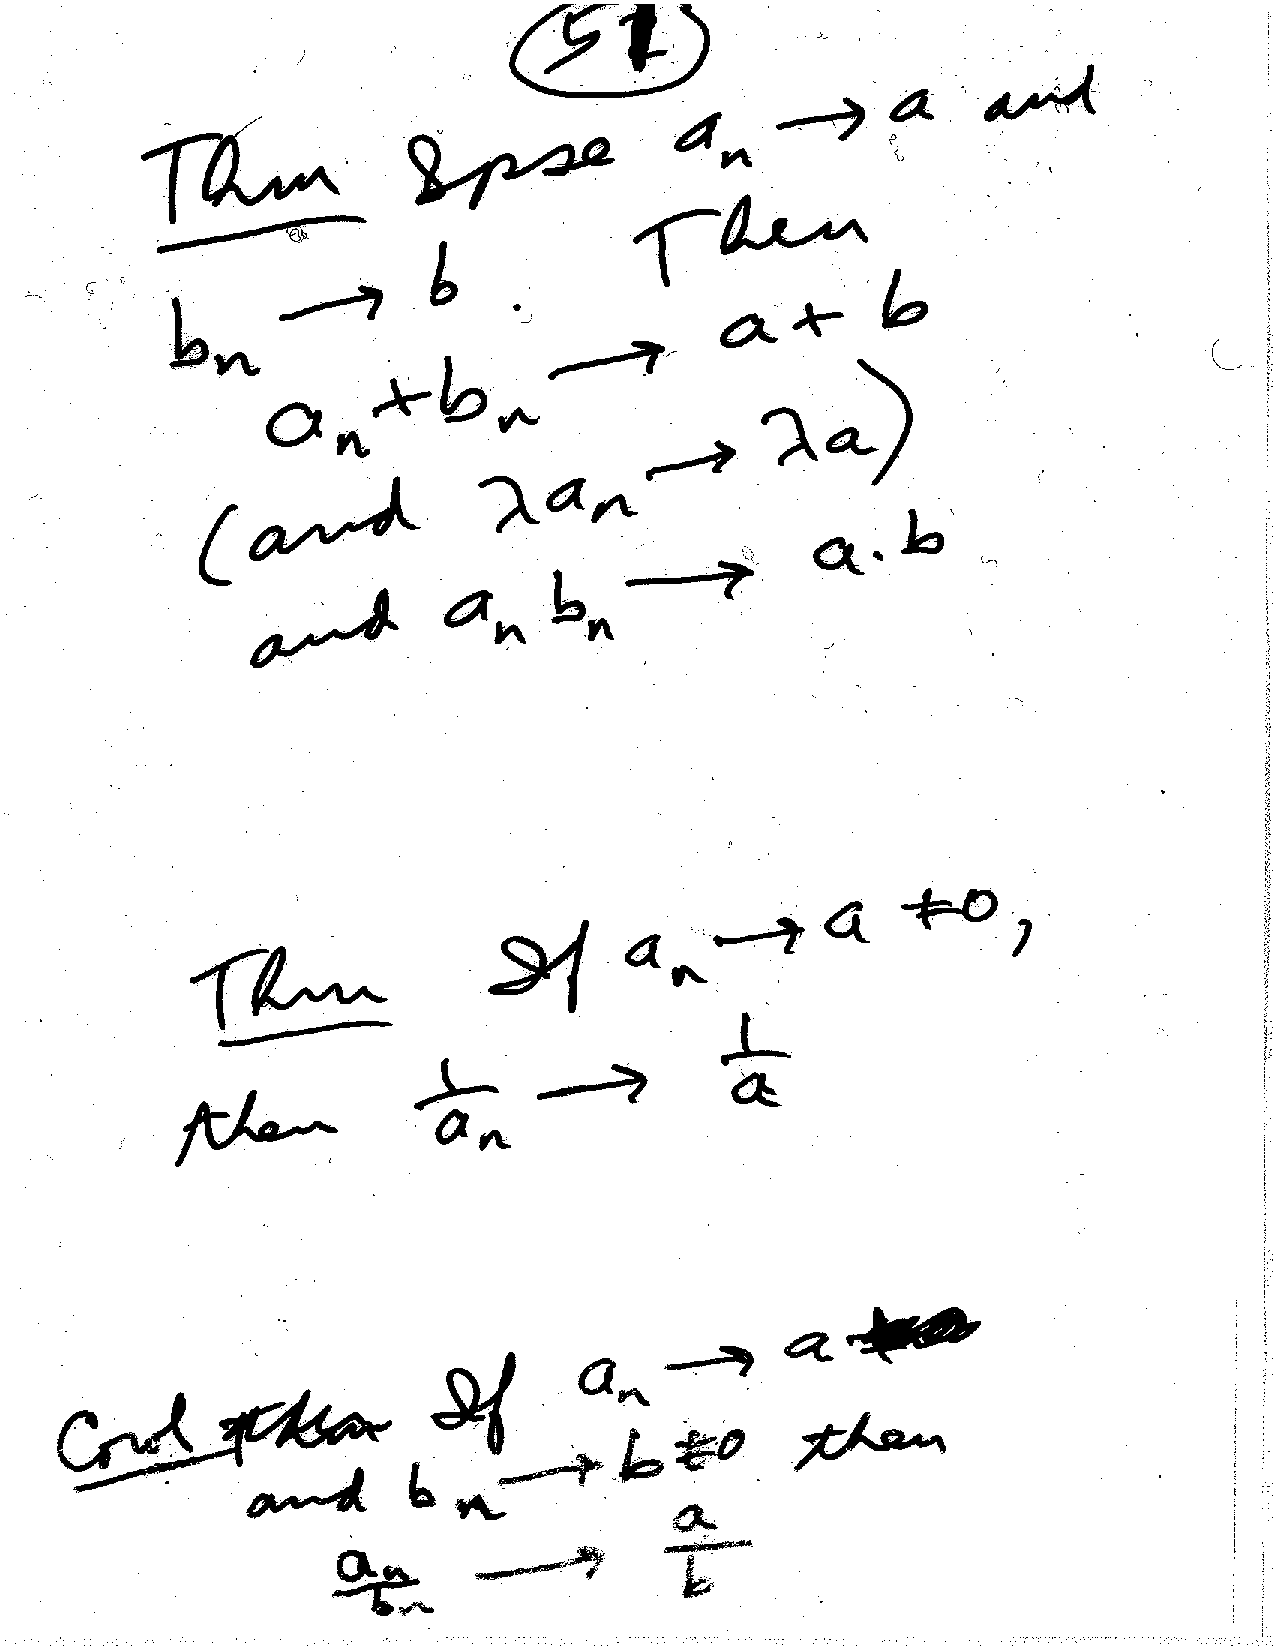
\includegraphics[scale=.5]{Pages/SL_7} 

\newpage
\underline{A method of proving corner:}\newline
\underline{monotone sequences} \newline
Lat $\{a_n\}$ be a sequence of reals. We say $\{a_n\}$ is \underline{monotonic} if either $a_1 \leq a_2 ... \leq a_a \leq ...$
or else $a_1 \geq  a_2 ... \geq a_a \geq ...$ 
In the first case $\{a_n\}$ is said to be (monotone) \underline {non-decreasing} \textnormal and in the second case it is (monotone) \underline{non-increasing}. \underline{Theorem} suppose $a_n$ is monotonic and \underline{bowled}. Then it conveys in R.

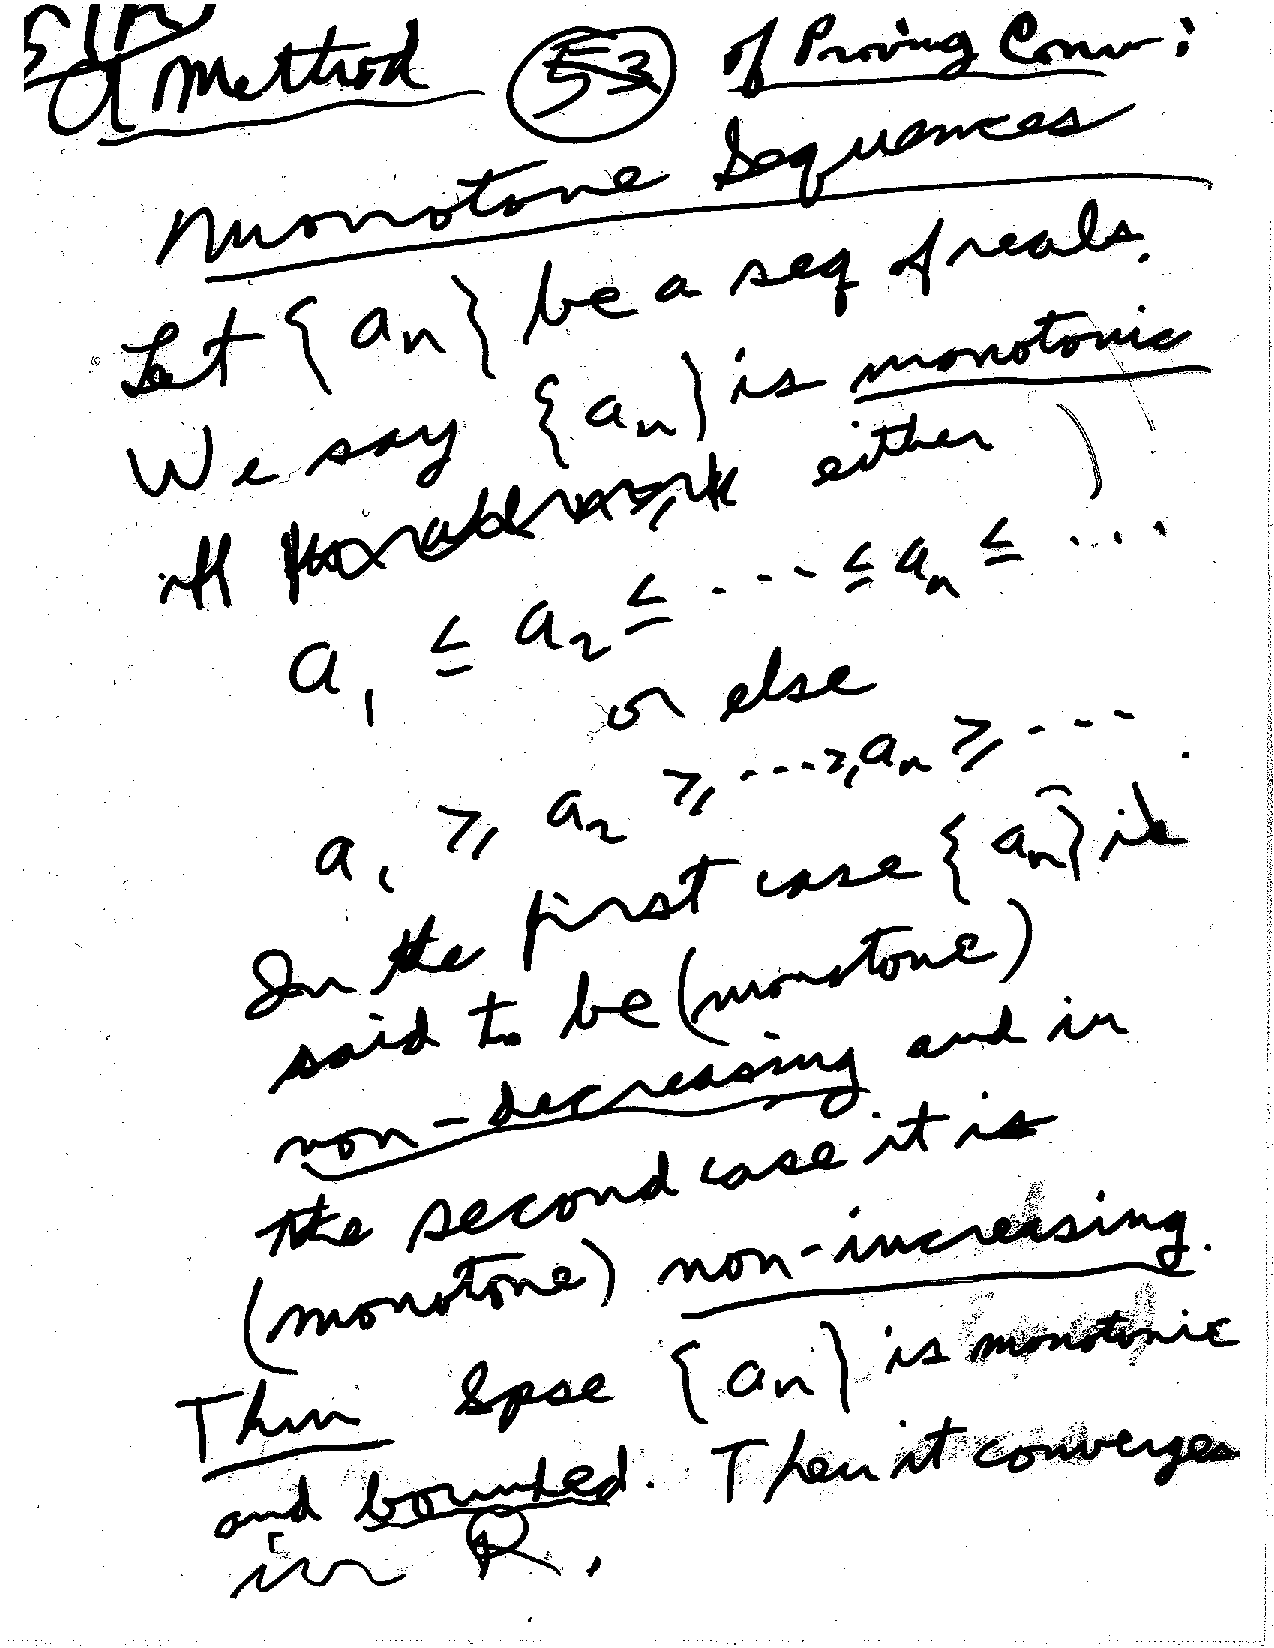
\includegraphics[scale=.5]{Pages/SL_8} 

\newpage
\underline{Theorem} Let $\{a_n\}$ be monotonic in R. Then in $R_\infty$\newline
$\lim_{n\rightarrow \infty}$ $a_n = 
\begin {cases}
sup $ $\{a_k\}$ $ & if a_1 \leq a_2 \leq a_3 \leq ...\\
inf $ $\{a_k\}$ $ & if a_1 \geq a_2 \geq ... 
\end {cases}$

\underline{Pf:} W l.o.g suppose $a_1 \leq a_2 \leq$ take away $b < suppose a_k$
Then $\exists k < \infty s.t. b < $ $\{a_k\}$. For all  $n \geq k, a_n \geq a_n so$
$a_n > b$. But also $a_n /leq suppose $ $\{a_k\}$

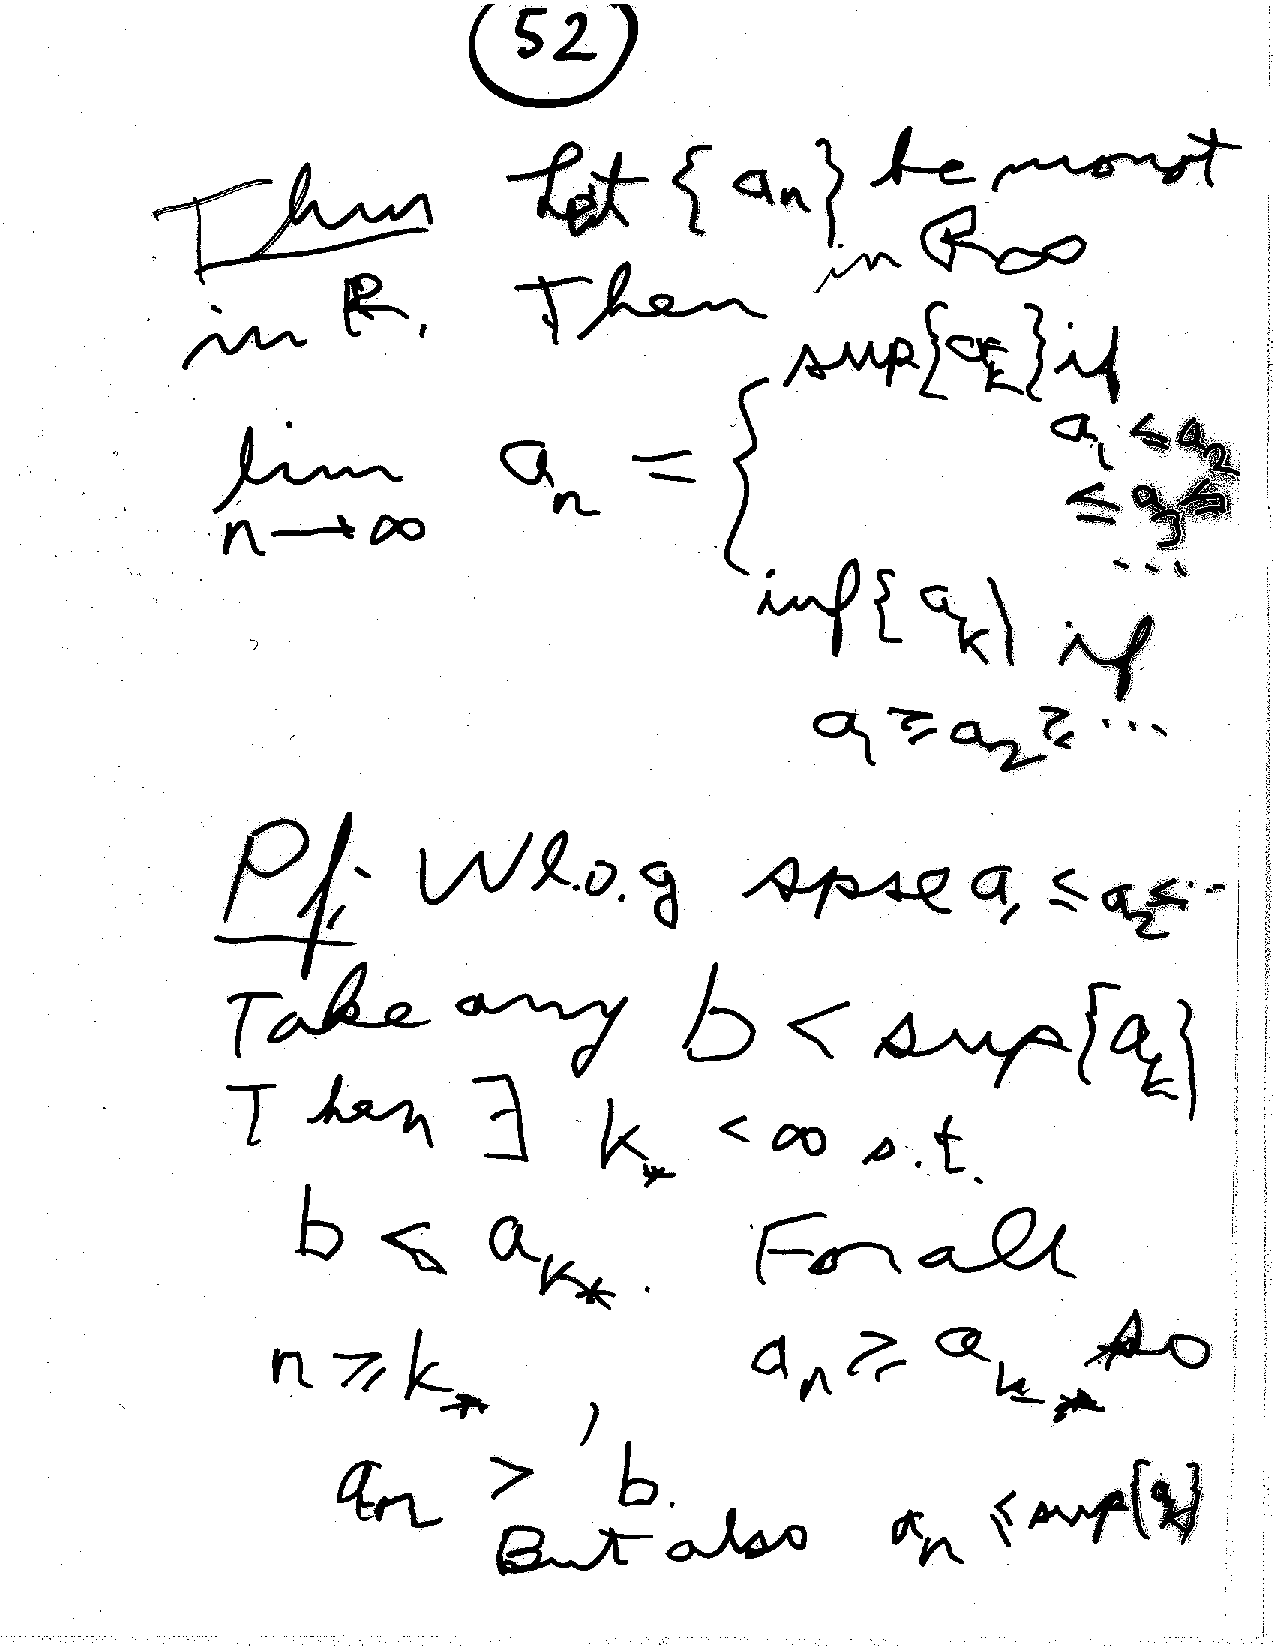
\includegraphics[scale=.5]{Pages/SL_9} 

\newpage

\underline{Theorem} Let $\{a_n\}$ be any sequence in $\mathbb{R}$ then $\exists 1 \leq n_1 < n_2 < ... s.t. a_{n_{1}}, a_{n_{2}},$ $a_{n_{3}}, ...$ is monotonic (i.e. $a_n$ has a monotonic sub sequence)\newline
\underline{Pf:} Either $a_1 \leq a_n$ for infinity many $n > 1$. Applying to each aj
Let J = $\{j\geq 1 : a_n \geq a_j$ for infinity many $n > j\}$
\underline{Cosel} $|J| = \infty $
Let $n_1$ = smallest $ j \in J$ $\exists n_2 > n_1$ with $n_2 /in J, ...$ ete get $ {n_k}$

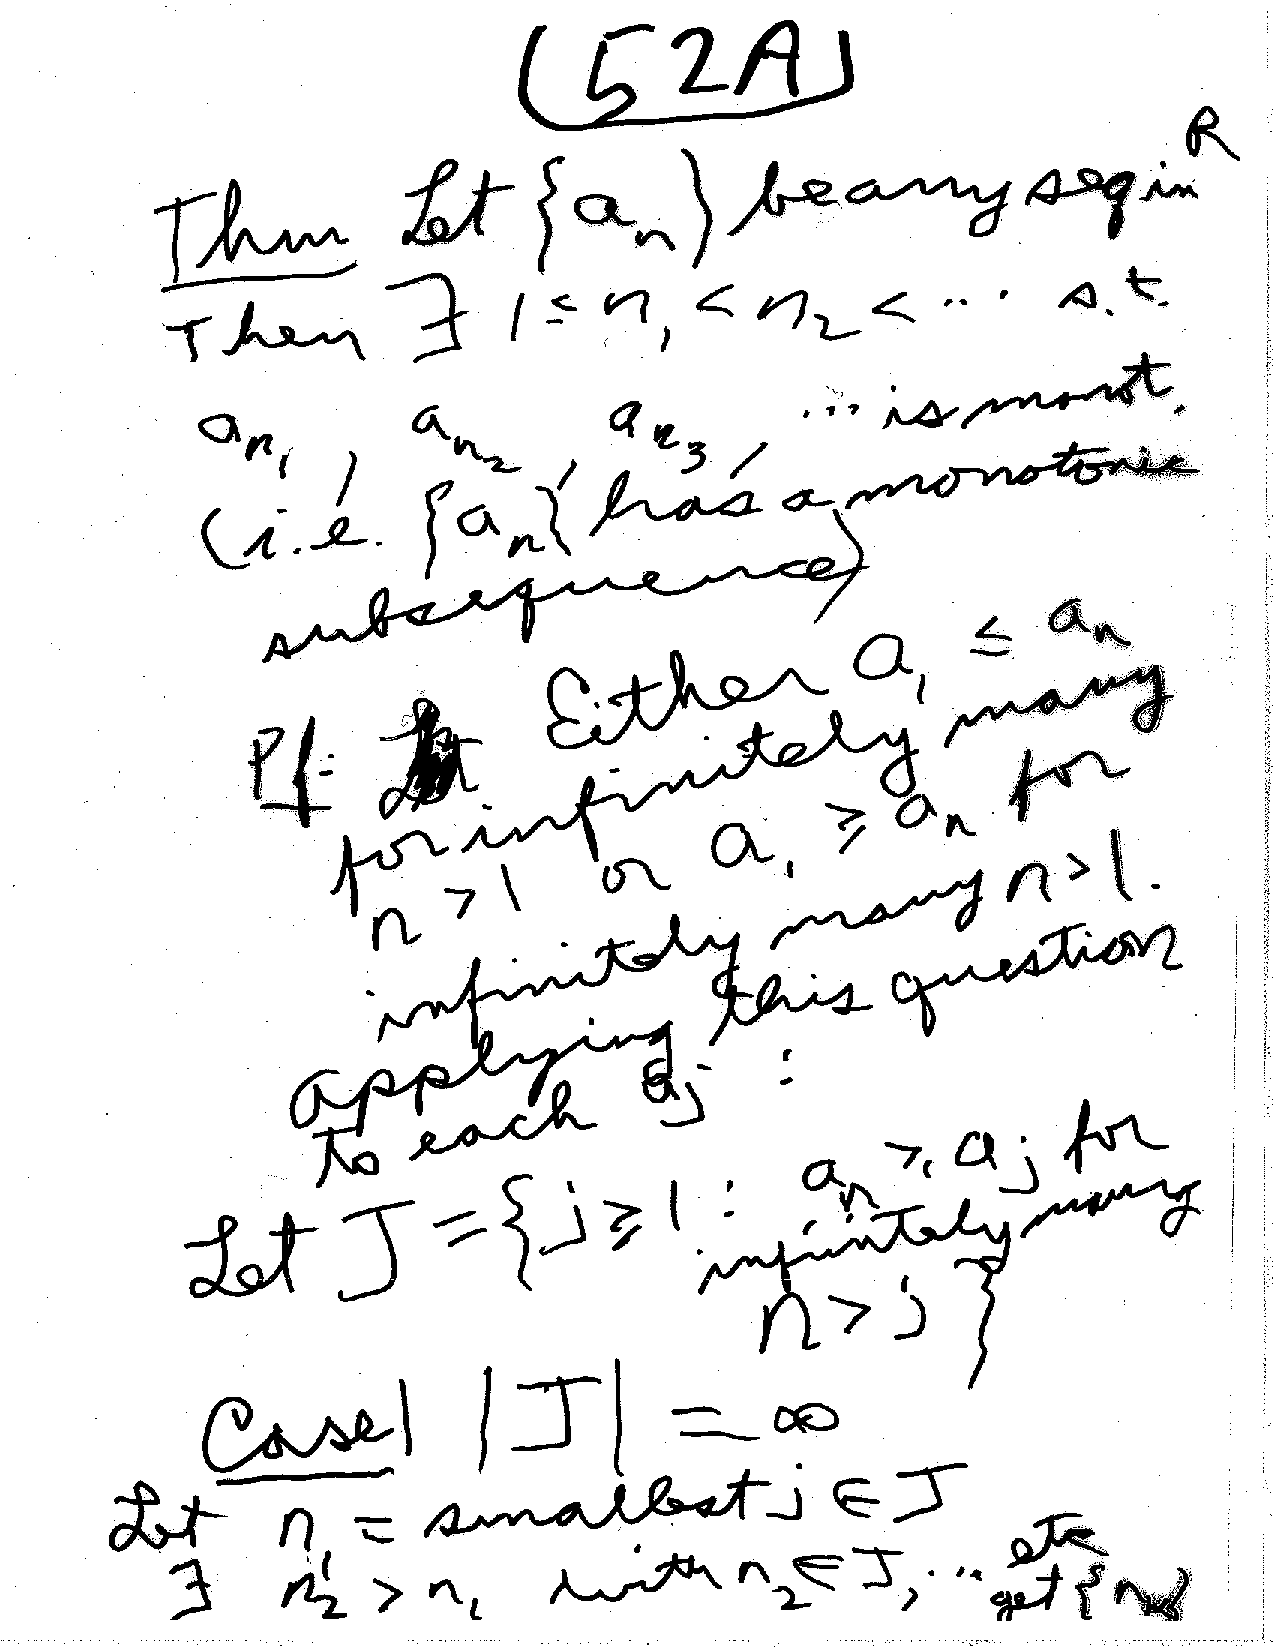
\includegraphics[scale=.5]{Pages/SL_10} 

\newpage

and $a_{n_{1}} \leq a_{n_{2}} \leq ...$ \newline
\underline{Case 2} $|J| < \infty$
take away $n_1 >$ one and max. $j \leftarrow J$ \newline
By construction, if $n_2$ is large enough $n_2 > n_1$ and $a_{n_{2}} < a_{n_{1}}$
By induction, having constructed $n_1 < n_2 < ... < n_k$ p.t. $a_{n_{1}} > a_{n_{2}} > ... > a_{n_{k}}$
$\exists n_{k+1} > n_k$ s.t. 
$a_{n_{k+1}} < a_{n_{k}}$ \newline
and so the theorem holds. 

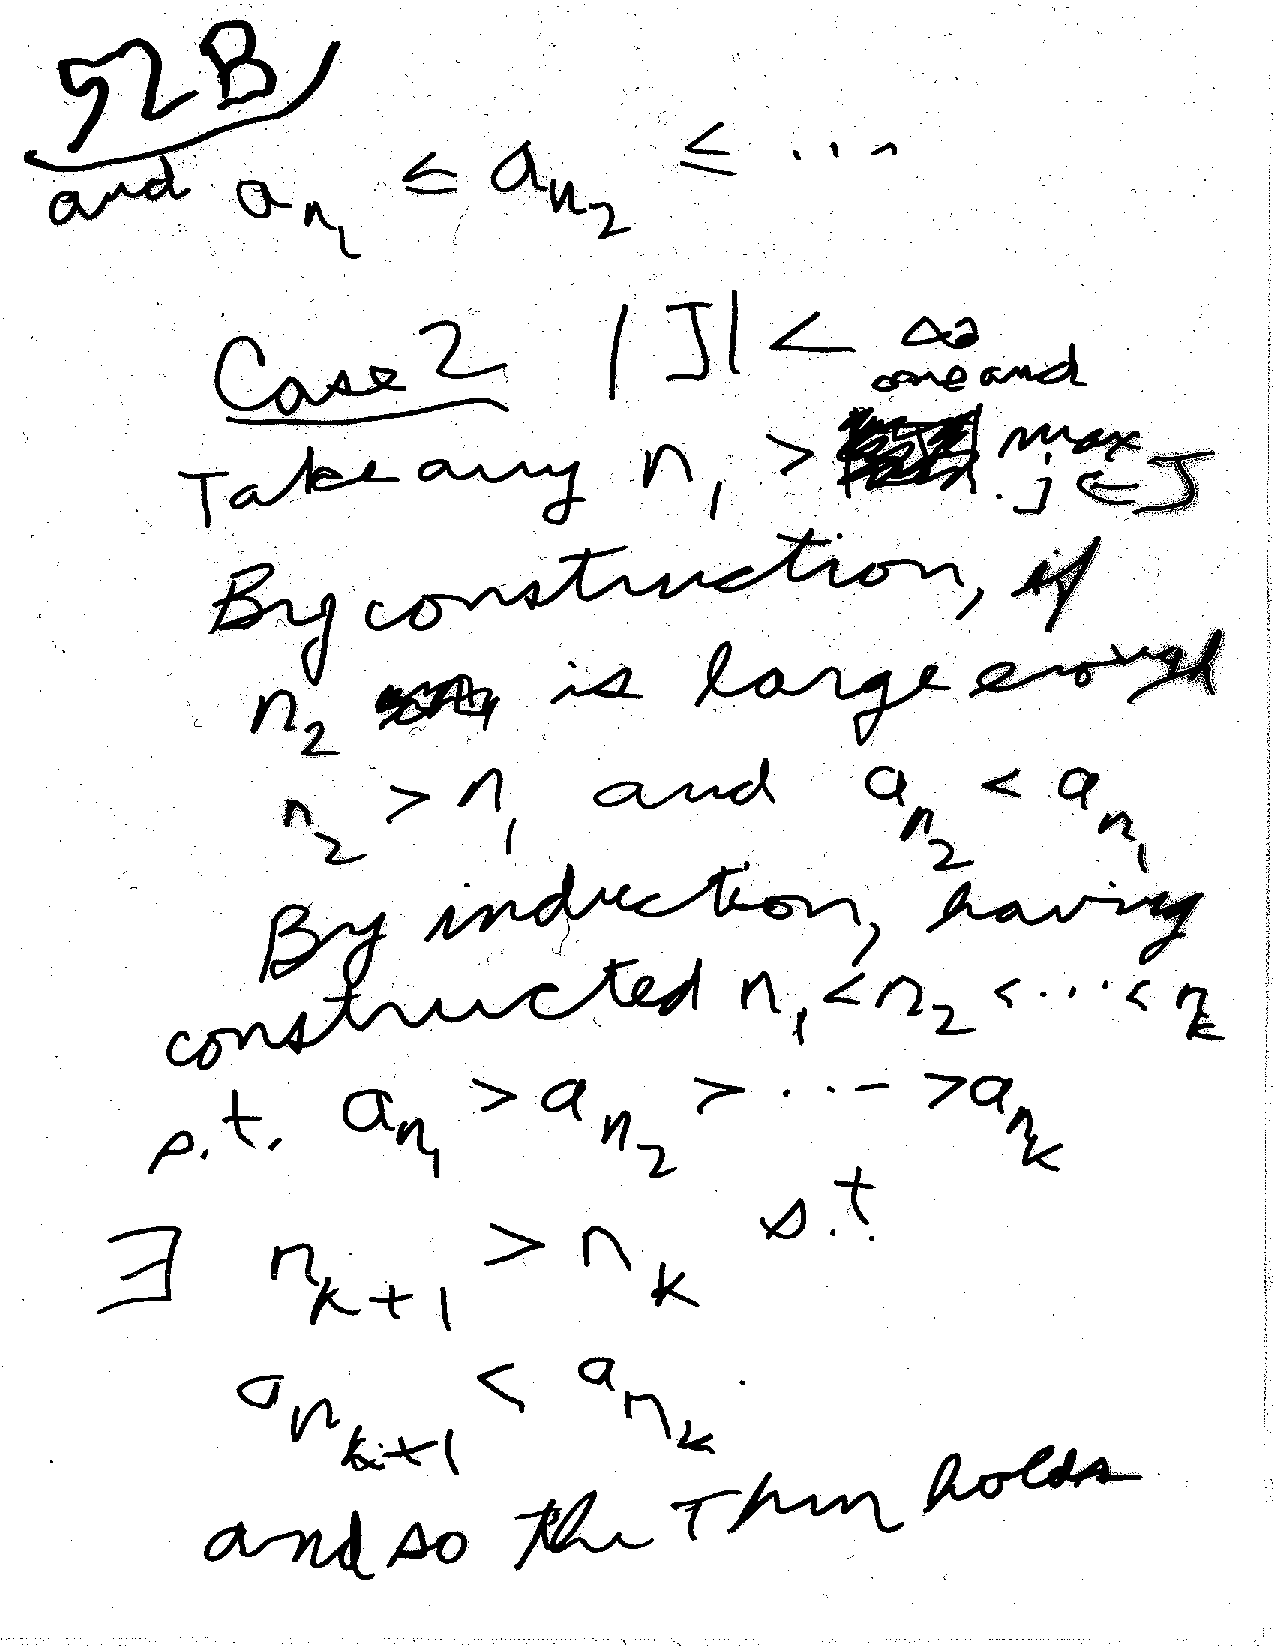
\includegraphics[scale=.5]{Pages/SL_11} 

\newpage
\section{Limit and Convergence}

%Joe: 50-51

%Quinten: 52-53
Therm Let $\{ a_n \}$ be monotonic
in $\mathbb{R}$. Then in $\mathbb{R}_{\infty}$
$\lim_{n \rightarrow{\infty}}$
$$a_n = \begin{cases} 
\sup \{ a_k \} & \mbox{if } a \leq a_2 \leq a_3 \leq...\\
\inf \{ a_k \} & \mbox{if } a\geq a_2 \geq...
\end{cases}$$

The limit is in  $\mathbb{R}$ if $\{ a_n \}$ is bounded


$\underline{Pf}$: WL.o.g spse  $a_1 \leq a_2 \leq ...$ Take any b $<$ sup $\{ a_k \}$ Then 

$\exists\ k_* < \infty$ s.t. $b < a{_k{_*}}$ for all $n \geq k_* , \{ a_n \} \geq 
 a{_k{_*}}$ so $ a_n > b.$ But also $a_n \leq a_n$
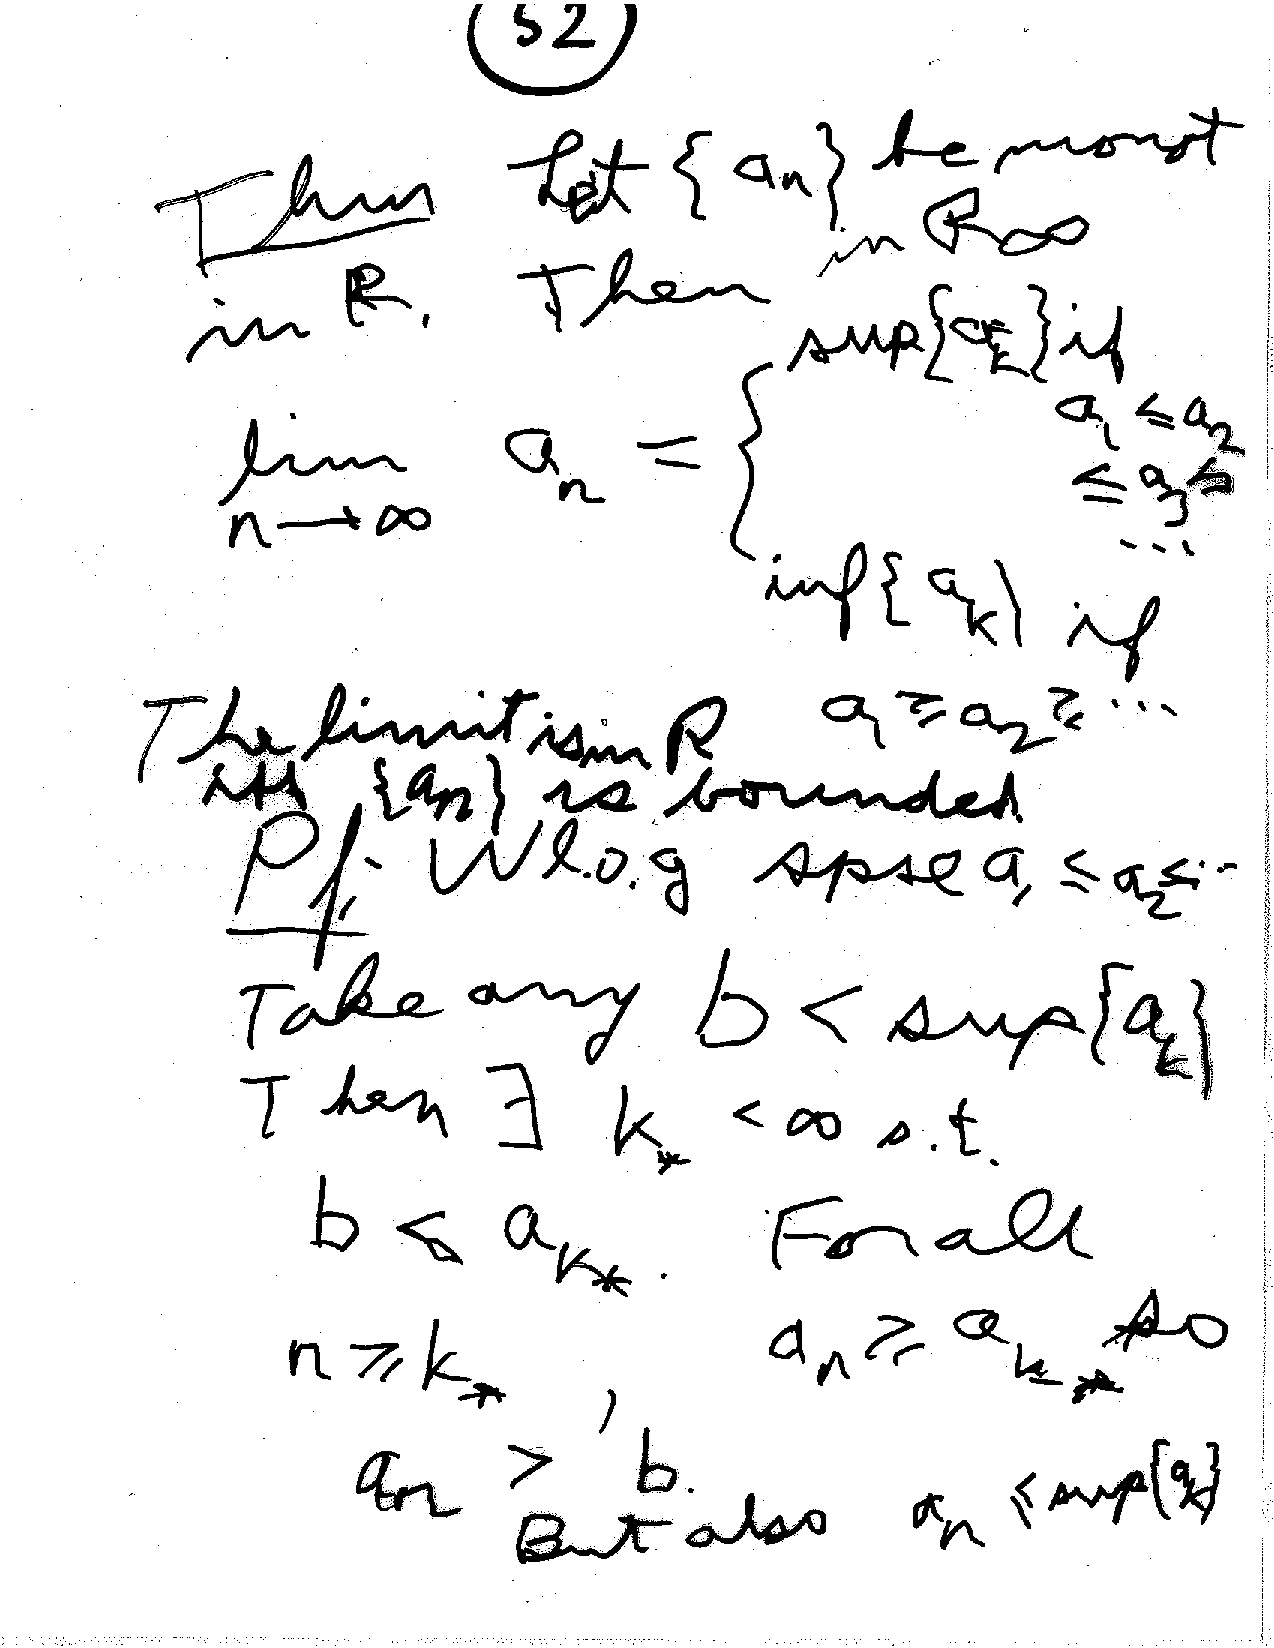
\includegraphics[scale=.5]{Pages/LC_6} 

\newpage
What if $\{ a_n \}$ is $\underline{not}$ monotonic?
$\underline{Therom}$ Let $\{ a_n \}$ be seq in $\mathbb{R}$.
Then $\exists$ 1 $\geq$ n, $<$ $n_2$ $<$ ... s.t. $a_{n_{1}}$,$a_{n_{2}}$, ... is monotonic.
$\underline{Pf}$: We need to consider the tail of a seq. Let 
$$\mbox{J} = \left\{ j \leq | : a_j > a_{j{t{k}}}\ for all\ K \leq 1 \right\}$$

If J is  unbounded we may write $\mbox{J} = \begin{cases} n_j & J\leq 1 \end{cases}$ where $1 \leq n_1 <n_2<...$
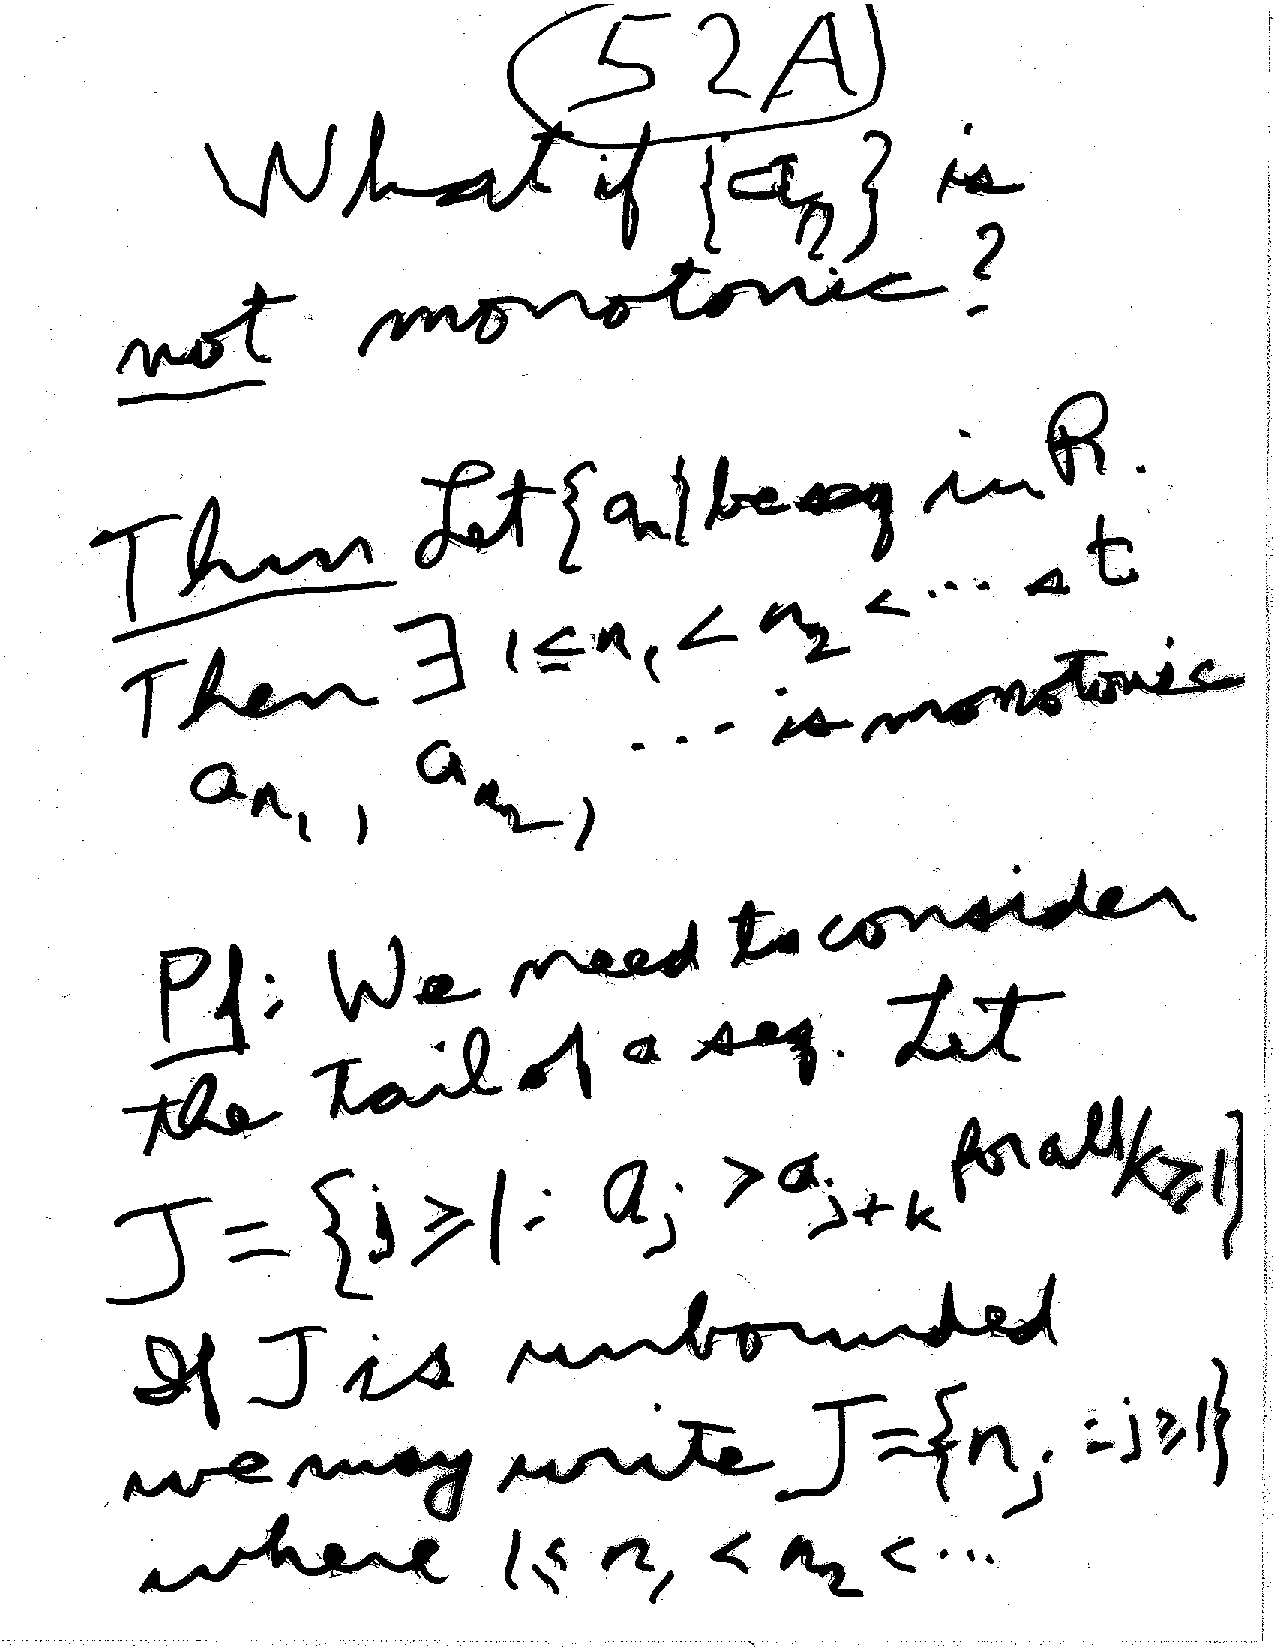
\includegraphics[scale=.5]{Pages/LC_7}

\newpage
By construction, $a_{n_{1}} > a_{n_{2}} >$ ... on the other hand, if $|J| < \infty$, let $n_1 \geq 1$ exceed every j $\in$ J. Having constructed $n_1 < n_2 < ... < n_k$ with $a_{n_{1}} \leq a_{n_{2}} ... \leq a_{n_{K}}$ (since $n_k$ and J) $\exists$ $n_k + 1 > n_k$ s.t. $a_{n_{k}} + 1$, and the desired construction follows by induction.
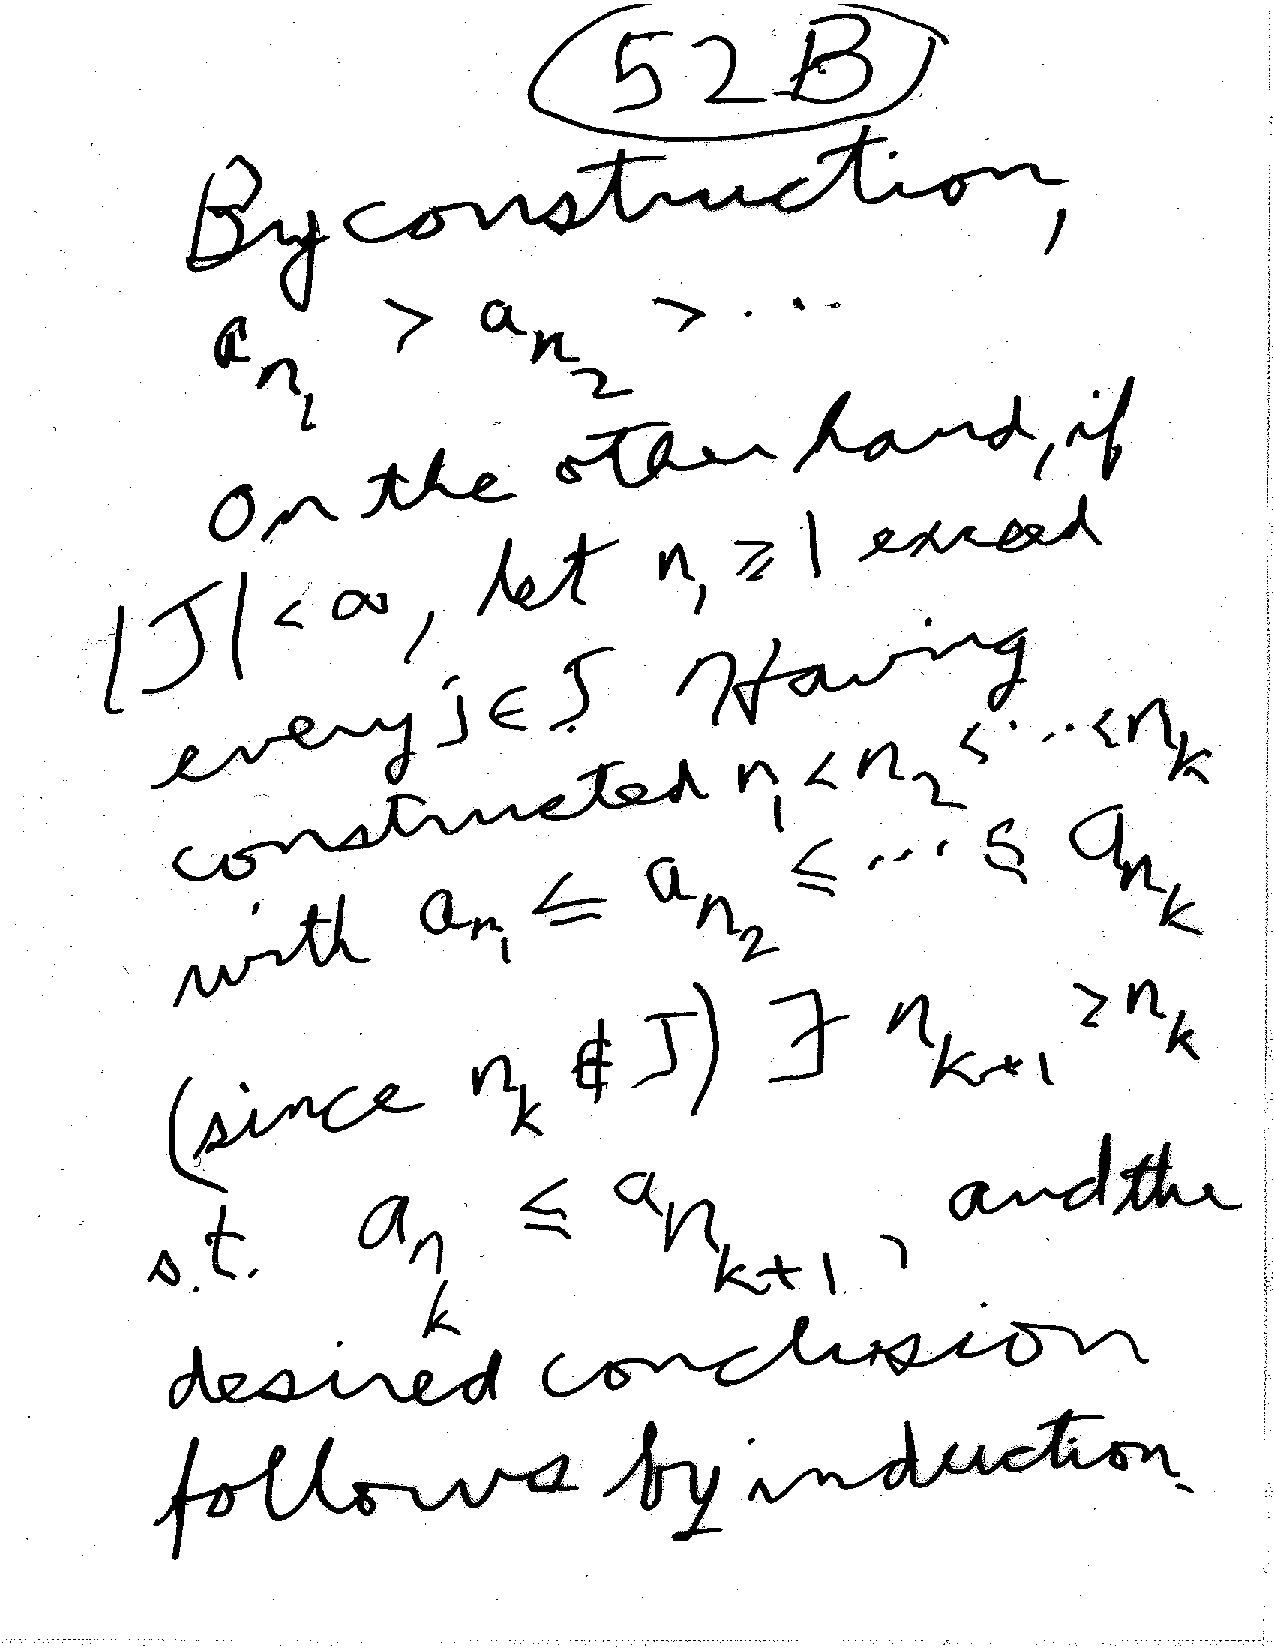
\includegraphics[scale=.5]{Pages/LC_8}

\newpage 
(Balzono weierstras) $\underline{Corllary}$ if $|a_n|$ is a bounded seq in $\mathbb{R}$, it has a covergent subsequence. (Even if $\{ a_n \}$ is $\underline{not}$ bounded, it has a subseq converging in $\mathbb{R}_\infty$.)
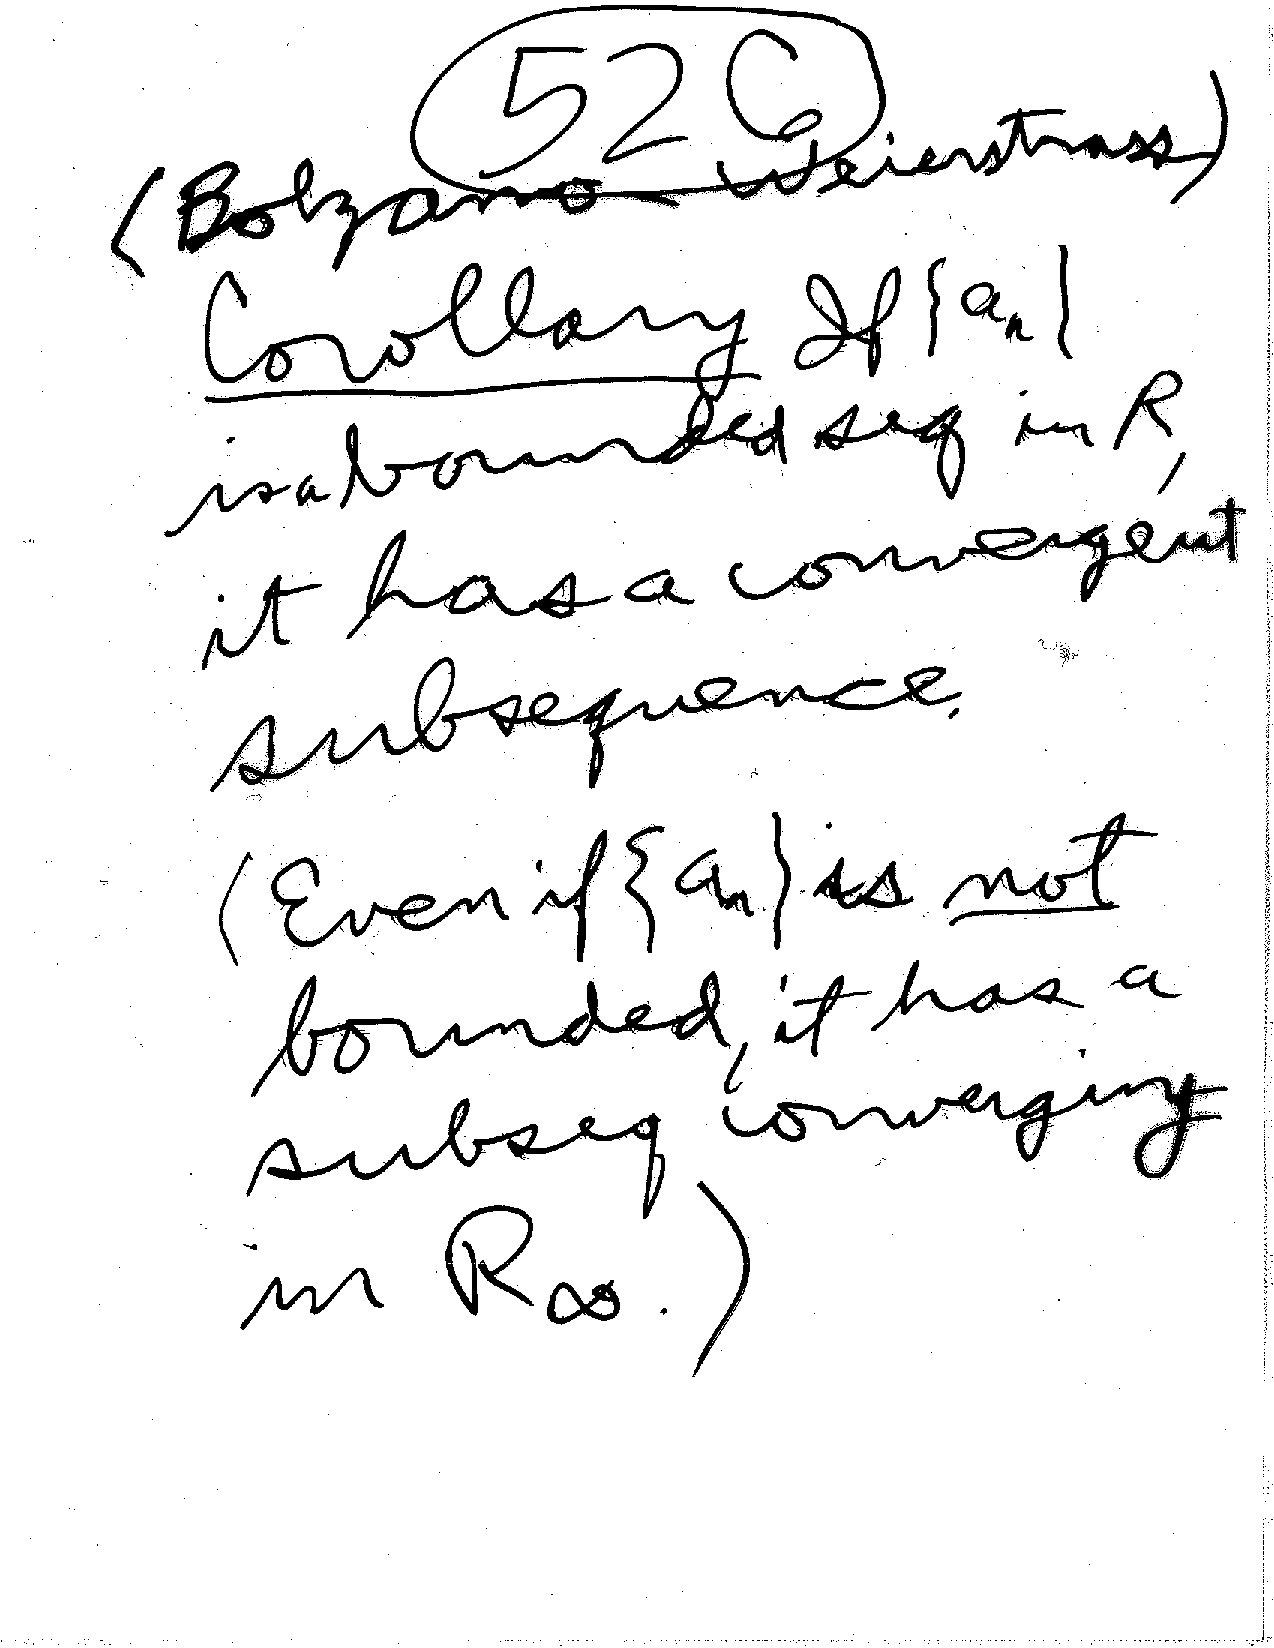
\includegraphics[scale=.5]{Pages/LC_9}

\newpage
$\underline{Cauchy Sequence}$ When can we gaurentee that a seq converges? $\underline{Def}$: a seq of vals $\{ x_n \}$ is said to be a $\underline{Cauchy seq}$ is $\forall \epsilon > 0 \exists N_\epsilon$ such that for every $n,m \geq N_\epsilon$ $$|x_n - x_m| < \epsilon$$ 
$\underline{Prop}$ Spse $x_n \rightarrow x$ Then $\{ x_n \}$ is a Cauchy seq.

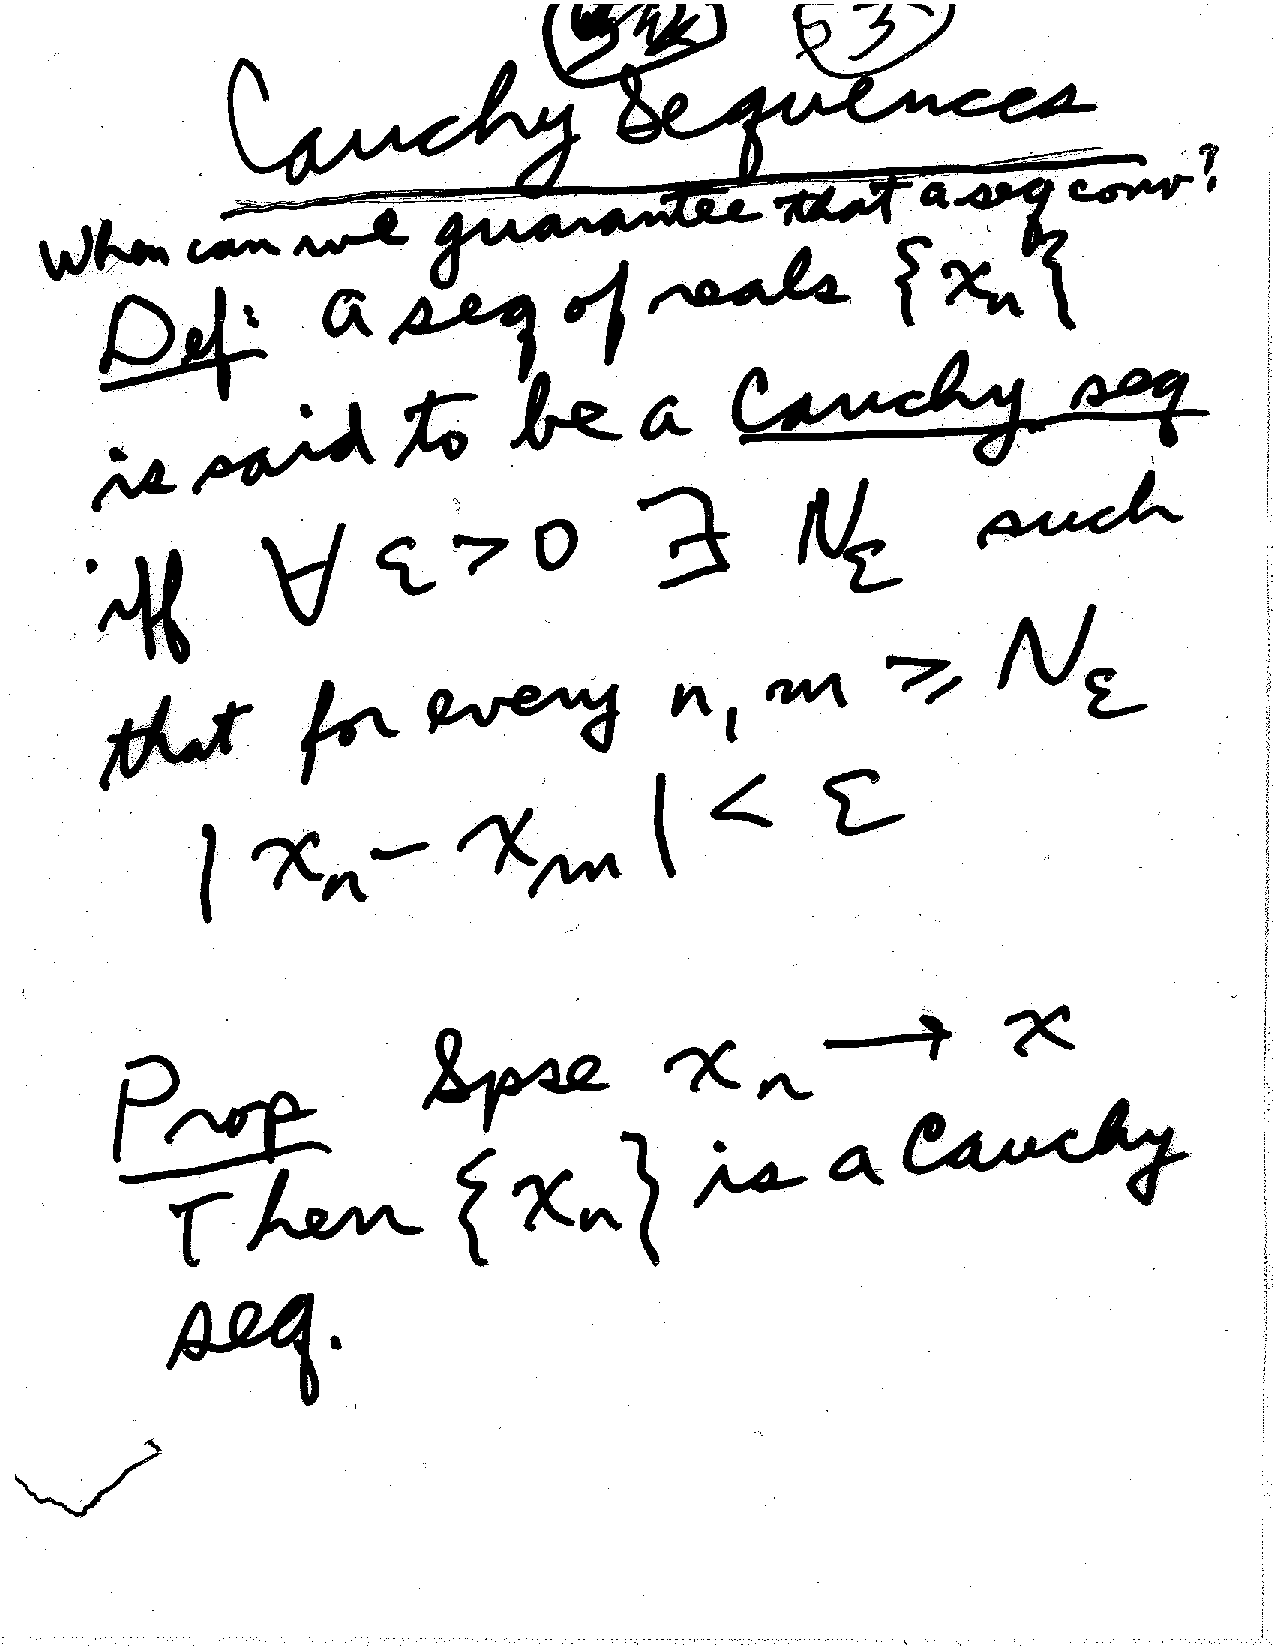
\includegraphics[scale=.5]{Pages/LC_10}

%Farishta: 53A-54A
\newpage
\section{Infinite Series}

%Sukhreet: IS1 - IS 7
A frog is 2 feet from a wall. He makes a succession of jumps toward it, always jumping half his remaining distance to the wall. Hence his finest jump is one foot. Now he is one foot from the wall. So

\includegraphics[scale=.5]{Pages/IS_1}

\newpage

his second jump is ${\frac{1}{2}}$ feet. He is now ${\frac{1}{2}}$ feet from the wall so he jumps ${\frac{1}{4}}$ feet. He makes successive jumps of ${1, \frac{1}{2}, \frac{1}{4}, \frac{1}{8}, . . .}$ After n jumps he has moved $$s_{n}=\sum_{j=1}^{n} {\frac{1}{2^{j-1}}}$$ feet. 

\includegraphics[scale=.5]{Pages/IS_2}

\newpage

and is now $${\frac{1}{2^{n-1}}}$$ feet from the wall so $${s_{n}=2-{\frac{1}{2^{n-1}}}}$$ If he keeps jumping forever, how far does he go? He moves $$\sum_{j=1}^{n} {\frac{1}{2^{j-1}}}$$ feet. This number is at most 2 and yet it exceeds $$2-{\frac{1}{2^{n}}}$$ for all $$n\geq1$$. 

\includegraphics[scale=.5]{Pages/IS_3}

\newpage

Hence the sum of this infinites collection of numbers ${1, \frac{1}{2}, \frac{1}{4}, . . .}$ must be two. How can we generalize this? 
\underline {Generalization 1}: Genetic Series 
How large is $1+r+r^{2}+$ . . . If $|r|<|$? Solution: Let $S{n}= 1+r+...+r^{n}$ For $r\leq 0$, $S{1}\leq S{2}\leq ...$ and we expect him $S_{n}=\sum_{j-0}^{\infty} {r^{j}}$ 

\includegraphics[scale=.5]{Pages/IS_4}

\newpage

$S_{n}=1+r+...+r^{n}$ is complex in that it has too many terms. how can we simplify it? We need to capitalize on the regularity of the expensive. 
Notice: $rS_{n}=r+r^{2}+...+r^{n+1}$, subtracting equals from equal $S_{n}-rS_{n}=1-r^{n+1}$ so for $r\neq 1, S_{n}=\frac{1-r^{n+1}}{1-r}$

\includegraphics[scale=.5]{Pages/IS_5}

%Matthew: IS8 - IS15

%Will: IS16 - IS23

\newpage %16

\begin{center}

{Infinite Series 16}

\end{center}

(ie) Suppose $r_{*} > 1$

Take $1 < \lambda < r_{*}$

$\exists N:N>N$

$=> |{\frac{{^a}n+1}{an}}| = \lambda$

We assume this means

$|a_{n}| > O$ for $n \geq N$

ntense $|{^a}N+K|\geq \lambda {^k}$

for $k\geq1$ so that

$|{^a}N+K|->\infty$ and $N+K-$

goes to infinity

this $\Sigma$an diverges

\begin{center}

\includegraphics[scale=1]{Pages/IS_16}

\end{center}

\newpage %17

\begin{center}

Infinite Series 17

\end{center}

Case 1

\begin{center}

$(iii) a_{n} = n$ $r_{what} = r^{what} = 1$

$\Sigma a_{n} = \infty$ 

\end{center}

Case 2

\begin{center}

$a_{n} = \frac{1}{n^{2}}$ $r_{*} = r^{*} = 1$

yet $\Sigma a_{n} < \infty$

Pf: $= \infty \Sigma n=1 \frac{1}{n{2}} \leq \infty \Sigma n=1 \frac{2}{n(n+1)}$

\end{center}

$=lim 2 N n=1 \Sigma ({\frac{1}{n}}-{\frac{1}{n+1}})$

$=lim {\underset{\text{$N\Rightarrow \infty$}}{lim 2}}(1-\frac{1}{N+1})$

$=2<\infty$

Hence a series for which $r_{*}\leq 1\leq r^{*}$ is either common div?
\begin{center}

\includegraphics[scale=.7]{Pages/IS_17}

\end{center}

\newpage %18

\begin{center}

Infinite Series 18

\end{center}

A refinement of the ratio teat, the Root Test does not 
require that evenly excessive ratio is "well-behaved", but merely that some p-what preponderance are.
{\underline {Then}} let r $=$ ${\underset{\text{$N\Rightarrow \infty$}}{lim}}|a_{n}|^\frac{1}{n}$

(i) if $r<1$ the something corns absolutely

(ii) if $r>1$ the something diverges

(iii) if $r=1$ the test is inconclusive

\begin{center}

\includegraphics[scale=.7]{Pages/IS_18}

\end{center}

\newpage %19

\begin{center}

Infinite Series 19

\end{center}

Pf: (i) Suppose $r<1$ and take any $r<\lambda <1$

$\exists N: n \geq N => |a_{n}|^{\frac{1}{n}} \leq \lambda$

ntense $|a_{n}| \leq what^{n}$

By the comparison test $\Sigma a_{n}$ comes ahead.

(ii) Suppose $r>1$ and the $1<\lambda<r$

For {\underline {any}} $N < \infty$

$\exists n > N : |a_{n}|^{\frac{1}{n}} \geq what$

ntence lim says $|a_{n}| = \infty$

$n->\infty$

$\Sigma a_{n} diveges$

(iii) if $r=1$, test fail

\begin{center}

\includegraphics[scale=.7]{Pages/IS_19}

\end{center}

\newpage %20

\begin{center}

Infinite Series 20

{\underline {Power Series}}

\end{center}

Let $f(x) = \infty \Sigma$ $n=0$ $a_{n}x^{n}$

Let $R = {\frac{1}{lim}}|a_n|^{\frac{1}{n}}$

Then

(i) series comes absol for $o\leq |x|<R$

(ii) series div for ${x}>R$

(iii) at $x=R$ we may have common div

$O\leq R\leq \infty$ . R is called the radius of com of the power series.
\begin{center}

\includegraphics[scale=.7]{Pages/IS_20}

\end{center}

\newpage %21

\begin{center}

Infinite Series 21

\end{center}

{\underline {PF:}} By Root Test,

$\Sigma a_{n} x^{n} lone something$

if ${\underset{\text{$N\Rightarrow \infty$}}{\bar{lim}}}$ $|a_{n} x^{n}|^{\frac{1}{n}}<1$

if $|x|$ ${\underset{\text{$N\Rightarrow \infty$}}{\bar{lim}}}$ $|a_{n}|^{\frac{1}{n}}$

if $|x|$ $<$ ${\frac{1}{lim|a_{n}|}^{\frac{1}{n}}}$

if $|x|$ $lim n->\infty$ ${|a_{n}}|^{\frac{1}{n}}$

if $|x|$ $<$ ${\frac{1}{lim}}{|a_{n}}|^{\frac{1}{n}} = R$

If ${\bar{lim}}$ ${|a_{n}x^{n}}|{\frac{1}{n}} > 1$ soive div

And series div if $|x| > R$ 

When $|x| = R$ anything can happen
\begin{center}

\includegraphics[scale=.7]{Pages/IS_21}

\end{center}
\newpage %22

\begin{center}

Infinite Series 22

For Series $\Sigma$ $a_{n} st.$ $a, \geq a_{z} \geq $ .. $\geq 0$ 

We can obtain two separate equal conditions chastening comes or div

{\underline {Thml}} (Cauchy Condoumsatism The)If $a_{1} \geq a_{2} \geq $ ... $\geq 0$ then

$\frac{1}{2}$ $\underset{\text{k=1}}{\overset{\text{$\infty$}}{\Sigma}}$ $\overset{\text{k}}{2a_{2k}}$ $\leq \underset{\text{n=1}}{\overset{\text{$\infty$}}{\Sigma}} {a_{n}}$ $\leq \underset{\text{k=0}}{\overset{\text{$\infty$}}{\Sigma}}$ $\overset{\text{k}}{2a_{2k}}$

ntense $\Sigma a_{n}$ and $\Sigma 2^{k}$ $a_{2k}$

consomething n divege something

\includegraphics[scale=.7]{Pages/IS_22}

\end{center}

\newpage %23

\begin{center}

Infinite Series 23

\underline{Pfi} $\underset{\text{k=1}}{\overset{\text{$\infty$}}{\Sigma}}$ ${a_{k}}$ $= \underset{\text{$\infty$=0}}{\overset{\text{$\infty$}}{\Sigma}}$
$({\underset{\text{$2^{n}\leq k < 2^{n+s}$}}{\Sigma a_{k}}})$

$\frac{1}{2}(2^{n+1}a_{2n+1}) \leq {\underset{\text{$2^{n}\leq k < 2^{n+1}$}}{\Sigma a_{k}}}$ $\leq 2^{n}a_{2n}$

Summing over $n \geq 0$ given

$\frac{1}{2}\underset{\text{n=1}}{\overset{\text{$\infty$}}{\Sigma}} 2^{n}a_{2n} \leq \underset{\text{k=1}}{\overset{\text{$\infty$}}{\Sigma}} a_{k}$ $\underset{\text{n=0}}{\overset{\text{$\infty$}}{\Sigma}}2^{n}a_{2n}$

\end{center}

Application

\begin{center}

$\Sigma \frac{1}{n} = \infty$ $iH \underset{\text{n=0}}{\overset{\text{$\infty$}}{\Sigma}}a_{k}$ $\leq \underset{\text{n=0}}{\overset{\text{$\infty$}}{\Sigma}}$ $1=\infty$

\includegraphics[scale=.7]{Pages/IS_23}

\end{center}

Since the RHS is infinite, so is the LHS

%Rebecca: IS24 - IS32

\normalsize

\newpage

\noindent \underline{Theorem 2} (The Integral Test)
\vspace{5mm}
\\ Suppose $a_1 \geq a_2 \geq \cdots \geq 0$.
\\ Extend $a_n$ to $a(x)$ where $a(x)$ is continuous,
$a(n) = a_n$ and $a(x)$ decreases,
\\ Then $\sum_n a_n < \infty$ if and only if $\int_{1}^{\infty} a(x) dx < \infty$
\vspace{5mm}
\\ \underline{Proof}
$$\int_{1}^{\infty} a(x) dx = \sum_{n=1}^{\infty} \int_{n}^{n+1} a(x) dx$$
$$ \leq \sum_{n=1}^{\infty} \int_{n}^{n+1} a_n dx$$
$$ = \sum_{n=1}^{\infty} a_n $$

\includegraphics[scale=.5]{Pages/IS_24}

\newpage

\noindent Lower-bounding,

$$ \int_{1}^{n} a(x) dx = \sum_{n=2}^{\infty} \int_{n-1}^{n} a(x) dx$$
$$ \geq \sum_{n=2}^{\infty} \int_{n-1}^{\infty} a_n dx $$
$$ = \sum_{n=2}^{\infty} a_n$$

\noindent Hence, $\sum_{n=2}^{\infty} a_n $ and $ \int_{1}^{\infty} a(x) dx$
\\ converge or diverge together.

\includegraphics[scale=.5]{Pages/IS_25}

\newpage

\noindent Are $\sum_{j=1}^{\infty} a_j$ and $ \sum_{k=1}^{\infty} b_k$ equal, where 
\\$$b_k = \sum_{n_k \leq j \leq n_{k+1}} a_j$$
and $n_o = 0 < 1 = n_1 < n_2 < \cdots $? 
\\ \vspace{2mm}

\noindent More generally, when do all re-orderings of the terms of a series produce the same sum?

\includegraphics[scale=.5]{Pages/IS_26}

\newpage

\noindent \underline{Theorem:} Let $a_j \geq 0$
\\ and $F_1 \subseteq F_2 \subseteq \cdots $ with
\\ $ \cup_{n=1}^{\infty} F_n = \mathbb{N} $ and $F_n$ is finite.
\\ Then $$\sum_{j=1}^{\infty} a_j = \lim_{n \rightarrow \infty} \sum_{j \in F_n} a_j$$
\vspace{5mm}
\\ \underline{Proof:} Take away
\\ $$ s < S_{\infty} \equiv \sum_{j=1}^{\infty} a_j$$
\\ $ \exists N < \infty$ such that for all 
\ $ n \geq N$, $a_1 + \cdots + a_n > s$

\includegraphics[scale=.5]{Pages/IS_27}

\newpage

\noindent Since $ \cup_{n=1}^{\infty} F_n = \mathbb{N}$, 
\\ $ \exists N' \geq N$ such that
\\ $\{1,2, \cdots, N\} \subseteq F_{N'}$ 
\\ Hence for all $ n \geq N'$
$$ \sum_{j \in F_n} a_j \geq \sum_{j=1}^{N} a_j > s $$
\\ \noindent Moreover, since $F_n$ is finite, 
$$\exists n* \geq max \{ j \in F_n \}$$
\\ Hence,$\sum_{ j \in F_n } a_j \leq \sum_{j=1}^{n} a_j \leq s_\infty $ \color{blue} TEXT CUT OFF \color{black}

\includegraphics[scale=.5]{Pages/IS_28}

\newpage

\textbf{Summation by Parts}
\vspace{2mm}
\\ \noindent \underline{Theorem} Let $A_o = 0$, $A_n = a_1 + \cdots + a_n$ 
\\ Suppose $\{ A_n: n\geq 1\}$ is bounded.
\\ Let $b_1 \geq b_2 \geq \cdots $ with $b_n \rightarrow 0.$
\\ \noindent Then $\sum_{j=1}^{\infty} a_j b_j$ converges.

\includegraphics[scale=.5]{Pages/IS_29}

\newpage

\begin{center}
(for all $n\geq 1$)
\end{center}
\vspace{3mm}
\noindent \underline{Proof:} Suppose $|A_n| < A^* <\infty$.
\\Fix any $\epsilon > 0$. Take any $\delta > 0$ to be chosen later $\exists  N$ such that for $n\geq N$ $0 \leq b_n < \delta_\epsilon$
\\ For $n \geq N$ and $p \geq 0$,
$$ \sum_{j=n}^{n+p} A_j b_j = \sum_{j=n-1}^{n+p} (A_j - A_{j-1}) b_j$$ 
$$= \sum_{j=n}^{n+p} A_j b_j - \sum_{j=n-1}^{n+p-1} A_j b_{j+1}$$

\includegraphics[scale=.5]{Pages/IS_30}

\newpage

\noindent So
$$|\sum_{j=n}^{n+p} a_j b_j|$$
$$ = |A_{n+p} b_{n+p} - A_{n-1} b_n + \sum_{j=n}^{n+p-1} A_j(b_j - b_{j+1})|$$
$$ \leq |A_{n+p}| b_{n+p} + |A_{n-1}| b_n + \sum_{j=n}^{n+p-1} |A_j| |b_j - b_{j+1}|$$

\includegraphics[scale=.5]{Pages/IS_31}

\newpage

$$\leq A^*\delta\epsilon + A^*\delta\epsilon + A^*\sum_{j=n}^{n+p-1} (b_j - b_{j+1})$$
$$ \leq 2A^*\delta\epsilon + A^*(b_n - b_{n+p})$$
$$ \leq 3A^*\delta\epsilon$$
\\ \noindent So let $\delta$ be any real number such that $0 < 3A^*\delta < 1$.
\\ \noindent Hence $\sum_{j=1}^n a_j b_j$ satisfies the Cauchy criterion. 
\\ Therefore, it converges.

\includegraphics[scale=.5]{Pages/IS_32}

\newpage

\noindent 3) Thinking grandly, maybe all of mathematics can be put on a set theoretic foundation.\\ \indent Let's try to do so. 
\\ \vspace{2mm}
\hrulefill

\noindent \underline{Some Set Theory}
\vspace{2mm}
\\ \noindent A set can be defined by 
\begin{enumerate} [(i)]
\item listing its elements
\item listing the properties that determine membership in the set.
\end{enumerate}

\includegraphics[scale=.5]{Pages/ST_9}

\newpage 

\noindent \underline{Examples}

\vspace{2mm}
\begin{itemize}
\item $\{1,2,5\}$ 
\item \{ cat, bat, dog\ \}
\item $\{\{1,2\},5\}$
\item \{ odd primes \}
\item \{ positive integers having no odd divisors \}
\end{itemize}

\includegraphics[scale=.5]{Pages/ST_10}

\newpage

\noindent How can we construct "new" sets from "old" sets?

\includegraphics[scale=.5]{Pages/ST_11_im1}

\noindent Clearly, $A$ defines another set $$ A^c \equiv \{ x \in \mathbb{U}: x \notin A\} $$

\includegraphics[scale=.5]{Pages/ST_11}

\newpage

\noindent So: What is a THEOREM?
\vspace{2mm}
\\ \noindent It always has the form 

\begin{center}
\fbox{If..., then...}
\end{center}

\vspace{2mm}
\noindent Let
\begin{itemize}
\item $A \equiv \{ x \in \mathbb{U}: x $ satisfies the conditions in the statement of the theorem \}
\item $B \equiv \{ x \in \mathbb{U}: x $ satisfies the conclusion of the theorem \}
\end{itemize}

\includegraphics[scale=.5]{Pages/ST_19}

\newpage

\noindent Hence, this theorem can be nested as nothing other than $A \subseteq B $.
\\ \indent Hence, a proof is just a logical demonstration:
\\ \indent For each $x \in A$, in fact $x \in B$ also.

\includegraphics[scale=.5]{Pages/ST_20}

\newpage

\noindent It is beyond the scope of this course to formalize how the statement $A \subseteq B$ may be proved. However, to illustrate what is required, it is sufficient to show:
\vspace{2mm}
\\ For each $x \in A$, there exists sets 
$$ D_{x, 1} \subseteq D_{x, 2} \subseteq D_{x, 3} \subseteq \cdots $$
\\ such that $x \in D_{x, 1}$ \underline{and}
$$ \bigcup_{j=1}^{\infty} D_{x, j} \subseteq B$$

\includegraphics[scale=.5]{Pages/ST_21}







 
%Maady: IS33 - IS42
\newpage 

\huge \underline{Corollary}

\large(estimating series)

\normalsize Let $b_1 \geq b_2 \geq$ ...,  $b_n \rightarrow 0$ 

then $$\sum_{j=1}^{\infty}(-1)^{j-1} b_j $$converges 

\underline{Proof:} $$A_n = \sum^n_{J=1}(-1)^{j-1}$$ is less 

Hence $$s_n = \sum^n_{J=1}(-1)^{j-1}b_j$$

converges in $R$,


$$0 \leq s_2 \leq s_4 \leq ..,$$

$$so$$ 

\includegraphics[scale=.42]{Pages/IS_33}


\newpage

$\exists d \leq s_\infty \le \infty$ such that

$s_n \rightarrow s_\infty$, moreover, 

$*s_{2n} \leq s_\infty \leq s_{2n-1}$

since $s_1 \geq s_3 \geq$ ...

consequently 

$|s_\infty - s_n| \leq b_{n+1}$

\includegraphics[scale=.42]{Pages/IS_34}


\newpage

\huge \underline{Power Series}

\normalsize let $$f(x) = \sum^{\infty}_{j=0}a_jx^j$$

Then $\exists 0\leq R \leq \infty$  such that

$$\sum^{\infty}_{j=0}a_jx^j$$ converges absolutely for $0 \leq |x| < R.$ and diverges for $|x|>R$

\includegraphics[scale=.42]{Pages/IS_35}

\newpage 

Proof:Want 
$|a_jx^j| \leq \lambda^j <1$ for converges 

So, taking $j^{th}$ roots,
need $|x| |a_j|^{\frac{1}{j}} \leq \lambda <1$ 

Need $$|x| \limsup_{j\rightarrow\infty} |a_j|^{\frac{1}{j}} <1$$

$$|x| < \frac{1}{\bar{\lim}_{j \rightarrow \infty} |a_j|^{\frac{1}{j}}} \equiv R$$

Proof $$|x|>R, \bar{\lim}_{J\rightarrow\infty}|x^ja_j|=\infty$$

\includegraphics[scale=.42]{Pages/IS_36}
 

\section{Metric Spaces Part 1}

%Travis: M1 - M5

%Jerome: M6- M10



\section{Metric Spaces Part 2}


%Bryant: M1-M7

%Reshma: M8-M14
\newpage
\Large
\center \underline{Reformulation} {\bf M8} \underline{Convergence}
\begin{flushleft}
We can use collections of points to determine whether a sequence converges. \\Let $D_r(x) = \{y\in M = d(x,y) <r\}$\\
\includegraphics[scale=.5]{Pages/MS_8_Im}
\\Fact: $$\lim_{n\rightarrow \infty} x_n = x $$ if and only if  
$\forall \varepsilon > 0 \exists N_{\varepsilon} < \infty: x_n \in D_{\varepsilon}(x)$\\for all n $\geqslant N_{\varepsilon}$
$D_r(x)$ is called the open disk (ball, sphere) of radius $r$ about $x$.\\
\includegraphics[scale=.4]{Pages/MS_8}
\newpage

Rudin calls it an r neighborhood of $x$, or just a neighborhood. Are there more general families of sets of points in a metric space ($m, d$) that could be used to determine convergence of sequences regardless of the particular sequence or its limit?
\includegraphics[scale=.5]{Pages/MS_9}
\newpage

For each point x of such a set $\mathcal{O}$, if $x_n \rightarrow x$ there must be an $\varepsilon_o > 0$ such that for all 0 $< \varepsilon < \varepsilon_o$ \\ $D_{\varepsilon}(x)\subseteq \mathcal{O}$ so that $X_n \in \mathcal{O}$ for all n sufficiently large.\\ \underline{Definition} $\mathcal{O}\subseteq \mathcal{M}$ is ($m,d$) an \underline{open set} in $\mathcal{M}$ if and only if $\forall x \in \mathcal{O } \exists E > 0$ such that $D_\varepsilon(X) \subseteq \mathcal{O}$\\
\includegraphics[scale=.5]{Pages/MS_10}
\newpage

For all metric spaces ($m,d$), $ \varnothing, \mathcal{M}$ and $D_r(x)$ for $x \in \mathcal{M}$ and $r \geq O$ are always open sets.\\
\center{ Properties of Open Sets}\\
\end{flushleft}
\begin{flushleft}
\begin{description}
  \item[(i)] Definition \{$\mathcal{O}_\alpha:\alpha \in J$\} are open in $\mathcal{M}$ so is $$ \bigcup_{\alpha \in J} \mathcal{O}_\alpha $$
  \item[(ii)] Definition $\mathcal{O}, \cdots, \mathcal{O}_n$ are open in $\mathcal{M}$ so is $$\bigcap^n_{j=1} \mathcal{O}_j$$ (Arbitrary unions of open sets are open. Intersections of finitely many open sets are open.) 
\end{description}
\includegraphics[scale=.4]{Pages/MS_11}
\newpage  
Definition $x$ is an \underline{interior point} of A $\subseteq M$ if an only if $\exists \varepsilon > 0: D_\varepsilon(x) \subseteq A $\\ $A^O =$ \{All interior points of A \} \underline{Fact: }$A^O$ is the largest open subset of $A$.\\ \underline{Definition} $x$ is a limit  point of $A\subseteq M$ if and only if $\forall \varepsilon>0 |D_\varepsilon(x) \bigcap A| \geq 2$ if an only if $\forall \varepsilon>0 (D_\varepsilon(x)\backslash \{x\}$)$\bigcap A \neq \emptyset$
\includegraphics[scale=.5]{Pages/MS_12}
\newpage
\underline{Proposition} $x$ is a limit point of $A$ if and only if $\exists$ sequence of distinct points of $A$ that converges to $x$. \\ \underline{Definition} $F \subseteq M$ is \underline{closed} if and only if every limit point of $F$ belongs to $F$.
\includegraphics[scale=.5]{Pages/MS_13}
\newpage
Examples of closed sets in $\mathbb{R}^1$ and $\mathbb{R}^2$

$\emptyset$ and $M$ are always closed space $F_j$ and $F_{\alpha}$ are closed in $M$.
\begin{description}
\item[i] if $F_1, \cdots, F_n$ are closed, so is $$ \bigcup^n_{j=1} F_j$$
\item[ii] if $F_\alpha$ is closed for $\alpha \in J$ so is $$\bigcap_{\alpha \in J} F_\alpha$$
\includegraphics[scale=.5]{Pages/MS_14}
\end{description}
\newpage
How should we define $\partial E$, the boundary of a set E?

Certainly $\partial E \subseteq \overline{E}$ since the boundary could involve points of $E$ and points infinitesimally close to points of $E$. However, $\partial E = \partial E^c$ so $\partial E \subseteq \overline{(E^c)}$
\includegraphics[scale=.5]{Pages/MS_18}

\newpage
\underline{Definition} $\partial E = \overline{E} \bigcap \overline{(E^c)}$\\ $\partial E$ is called the \underline{boundary} of the set $E$. 

Can $\partial E \varsupsetneqq E$?

Fact: $\overline{E} = E \bigcup (\partial E)$
\line(1,0){330} \\
Suppose $E \subseteq F \subseteq M (m,d)$\\
\underline{Definition} $E$ is dense in F\\ if and only if $\overline{E} \supseteq F$\\ if and only if every point of $F$ in $E \bigcap$ is a limit point of $E$\\ if an only if $\forall x \in F \exists x_n \in$ such that $x_n \rightarrow x$\\ Then $E$ is dense in $F$
\includegraphics[scale=.4]{Pages/MS_19}

\end{flushleft}
%Ethan: M15-M21
\newpage

$$m15$$
\underline{Theorem} $F\subseteq M$ is closed if and only if $F^c$ is open
 
\underline{Pf} : $(\Rightarrow)$ Suppose F is closed if $F^c$ is not open $\exists  x \in F^c$ suppose that $\forall \in > o$ $\exists x_\in \neq x$ :
 $$x_\in \in D_\in (x) \bigcap F$$
Hence $x$ is a limit point of F But F contains all its limit points so $x \in F$ continued. Thus $F^c$ is open

\includegraphics[scale=.75]{Pages/MS2_15}
\newpage

$$m16$$

$(\Leftarrow)$ suppose $F^c$ is open if F is not closed $\exists$ sequence of distinct points $x_n$ of F which conveys to a point $x \notin F$.
Since $x \in F^c$ and $F^c$ is open

$\exists \in > 0$ such that $D_\in$ (x) $\subset F^c$ also $\exists N : x_n \in D_e(x)$ for all $n>N$ But then $x_v \in F \bigcap F^c = \emptyset$ continued. Hence F is closed.

\includegraphics[scale=.75]{Pages/MS2_16}
\newpage
$$m17$$

Define let E $\leq$ m. Let E' denote the limit points of E then $\overline{E}$, the closure
 of E, is defined to be E$\bigcup$E'
\begin{itemize}
\item Fact 1 $\overline{E}$ is closed
\item Fact 2 If F is closed and E $\leq$ F then $\overline{E} \leq$ F
\end{itemize}

Corollary $\overline{E}$ = $\bigcap$ F
$/{F closed : E \leq F /}$



\includegraphics[scale=.75]{Pages/MS2_17}






\end{document}